\documentclass[twoside]{book}

% Packages required by doxygen
\usepackage{fixltx2e}
\usepackage{calc}
\usepackage{doxygen}
\usepackage[export]{adjustbox} % also loads graphicx
\usepackage{graphicx}
\usepackage[utf8]{inputenc}
\usepackage{makeidx}
\usepackage{multicol}
\usepackage{multirow}
\PassOptionsToPackage{warn}{textcomp}
\usepackage{textcomp}
\usepackage[nointegrals]{wasysym}
\usepackage[table]{xcolor}

% Font selection
\usepackage[T1]{fontenc}
\usepackage[scaled=.90]{helvet}
\usepackage{courier}
\usepackage{amssymb}
\usepackage{sectsty}
\renewcommand{\familydefault}{\sfdefault}
\allsectionsfont{%
  \fontseries{bc}\selectfont%
  \color{darkgray}%
}
\renewcommand{\DoxyLabelFont}{%
  \fontseries{bc}\selectfont%
  \color{darkgray}%
}
\newcommand{\+}{\discretionary{\mbox{\scriptsize$\hookleftarrow$}}{}{}}

% Page & text layout
\usepackage{geometry}
\geometry{%
  a4paper,%
  top=2.5cm,%
  bottom=2.5cm,%
  left=2.5cm,%
  right=2.5cm%
}
\tolerance=750
\hfuzz=15pt
\hbadness=750
\setlength{\emergencystretch}{15pt}
\setlength{\parindent}{0cm}
\setlength{\parskip}{3ex plus 2ex minus 2ex}
\makeatletter
\renewcommand{\paragraph}{%
  \@startsection{paragraph}{4}{0ex}{-1.0ex}{1.0ex}{%
    \normalfont\normalsize\bfseries\SS@parafont%
  }%
}
\renewcommand{\subparagraph}{%
  \@startsection{subparagraph}{5}{0ex}{-1.0ex}{1.0ex}{%
    \normalfont\normalsize\bfseries\SS@subparafont%
  }%
}
\makeatother

% Headers & footers
\usepackage{fancyhdr}
\pagestyle{fancyplain}
\fancyhead[LE]{\fancyplain{}{\bfseries\thepage}}
\fancyhead[CE]{\fancyplain{}{}}
\fancyhead[RE]{\fancyplain{}{\bfseries\leftmark}}
\fancyhead[LO]{\fancyplain{}{\bfseries\rightmark}}
\fancyhead[CO]{\fancyplain{}{}}
\fancyhead[RO]{\fancyplain{}{\bfseries\thepage}}
\fancyfoot[LE]{\fancyplain{}{}}
\fancyfoot[CE]{\fancyplain{}{}}
\fancyfoot[RE]{\fancyplain{}{\bfseries\scriptsize Generated by Doxygen }}
\fancyfoot[LO]{\fancyplain{}{\bfseries\scriptsize Generated by Doxygen }}
\fancyfoot[CO]{\fancyplain{}{}}
\fancyfoot[RO]{\fancyplain{}{}}
\renewcommand{\footrulewidth}{0.4pt}
\renewcommand{\chaptermark}[1]{%
  \markboth{#1}{}%
}
\renewcommand{\sectionmark}[1]{%
  \markright{\thesection\ #1}%
}

% Indices & bibliography
\usepackage{natbib}
\usepackage[titles]{tocloft}
\setcounter{tocdepth}{3}
\setcounter{secnumdepth}{5}
\makeindex

% Hyperlinks (required, but should be loaded last)
\usepackage{ifpdf}
\ifpdf
  \usepackage[pdftex,pagebackref=true]{hyperref}
\else
  \usepackage[ps2pdf,pagebackref=true]{hyperref}
\fi
\hypersetup{%
  colorlinks=true,%
  linkcolor=blue,%
  citecolor=blue,%
  unicode%
}

% Custom commands
\newcommand{\clearemptydoublepage}{%
  \newpage{\pagestyle{empty}\cleardoublepage}%
}

\usepackage{caption}
\captionsetup{labelsep=space,justification=centering,font={bf},singlelinecheck=off,skip=4pt,position=top}

%===== C O N T E N T S =====

\begin{document}

% Titlepage & ToC
\hypersetup{pageanchor=false,
             bookmarksnumbered=true,
             pdfencoding=unicode
            }
\pagenumbering{alph}
\begin{titlepage}
\vspace*{7cm}
\begin{center}%
{\Large mrgsolve }\\
\vspace*{1cm}
{\large Generated by Doxygen 1.8.13}\\
\end{center}
\end{titlepage}
\clearemptydoublepage
\pagenumbering{roman}
\tableofcontents
\clearemptydoublepage
\pagenumbering{arabic}
\hypersetup{pageanchor=true}

%--- Begin generated contents ---
\chapter{Main Page}
\label{index}\hypertarget{index}{}Documentation for mrgsolve C++ code. 
\chapter{Module Index}
\section{Modules}
Here is a list of all modules\+:\begin{DoxyCompactList}
\item \contentsline{section}{mrgx namespace}{\pageref{group__mrgx}}{}
\end{DoxyCompactList}

\chapter{Hierarchical Index}
\section{Class Hierarchy}
This inheritance list is sorted roughly, but not completely, alphabetically\+:\begin{DoxyCompactList}
\item \contentsline{section}{Comp\+Rec}{\pageref{struct_comp_rec}}{}
\item \contentsline{section}{databox}{\pageref{structdatabox}}{}
\item \contentsline{section}{dataobject}{\pageref{classdataobject}}{}
\item \contentsline{section}{datarecord}{\pageref{classdatarecord}}{}
\item \contentsline{section}{odepack\+\_\+dlsoda}{\pageref{classodepack__dlsoda}}{}
\begin{DoxyCompactList}
\item \contentsline{section}{odeproblem}{\pageref{classodeproblem}}{}
\end{DoxyCompactList}
\item \contentsline{section}{resim}{\pageref{structresim}}{}
\end{DoxyCompactList}

\chapter{Class Index}
\section{Class List}
Here are the classes, structs, unions and interfaces with brief descriptions\+:\begin{DoxyCompactList}
\item\contentsline{section}{\hyperlink{struct_comp_rec}{Comp\+Rec} \\*Functor for sorting data records in {\ttfamily reclist} }{\pageref{struct_comp_rec}}{}
\item\contentsline{section}{\hyperlink{structdatabox}{databox} }{\pageref{structdatabox}}{}
\item\contentsline{section}{\hyperlink{classdataobject}{dataobject} }{\pageref{classdataobject}}{}
\item\contentsline{section}{\hyperlink{classdatarecord}{datarecord} }{\pageref{classdatarecord}}{}
\item\contentsline{section}{\hyperlink{classodepack__dlsoda}{odepack\+\_\+dlsoda} }{\pageref{classodepack__dlsoda}}{}
\item\contentsline{section}{\hyperlink{classodeproblem}{odeproblem} }{\pageref{classodeproblem}}{}
\item\contentsline{section}{\hyperlink{structresim}{resim} \\*Resim functor }{\pageref{structresim}}{}
\end{DoxyCompactList}

\chapter{File Index}
\section{File List}
Here is a list of all documented files with brief descriptions\+:\begin{DoxyCompactList}
\item\contentsline{section}{inst/include/\hyperlink{dataobject_8h}{dataobject.\+h} }{\pageref{dataobject_8h}}{}
\item\contentsline{section}{inst/include/\hyperlink{datarecord_8h}{datarecord.\+h} }{\pageref{datarecord_8h}}{}
\item\contentsline{section}{inst/include/\hyperlink{mrgsolv_8h}{mrgsolv.\+h} }{\pageref{mrgsolv_8h}}{}
\item\contentsline{section}{inst/include/\hyperlink{mrgsolve_8h}{mrgsolve.\+h} }{\pageref{mrgsolve_8h}}{}
\item\contentsline{section}{inst/include/\hyperlink{odepack__dlsoda_8h}{odepack\+\_\+dlsoda.\+h} }{\pageref{odepack__dlsoda_8h}}{}
\item\contentsline{section}{inst/include/\hyperlink{odeproblem_8h}{odeproblem.\+h} }{\pageref{odeproblem_8h}}{}
\item\contentsline{section}{inst/include/{\bfseries Rcpp\+Include.\+h} }{\pageref{_rcpp_include_8h}}{}
\item\contentsline{section}{inst/include/\hyperlink{tofunptr_8h}{tofunptr.\+h} }{\pageref{tofunptr_8h}}{}
\item\contentsline{section}{inst/mrgx/\hyperlink{mrgx_8h}{mrgx.\+h} }{\pageref{mrgx_8h}}{}
\item\contentsline{section}{src/\hyperlink{dataobject_8cpp}{dataobject.\+cpp} }{\pageref{dataobject_8cpp}}{}
\item\contentsline{section}{src/\hyperlink{datarecord_8cpp}{datarecord.\+cpp} }{\pageref{datarecord_8cpp}}{}
\item\contentsline{section}{src/\hyperlink{devtran_8cpp}{devtran.\+cpp} }{\pageref{devtran_8cpp}}{}
\item\contentsline{section}{src/\hyperlink{mrgsolve_8cpp}{mrgsolve.\+cpp} }{\pageref{mrgsolve_8cpp}}{}
\item\contentsline{section}{src/\hyperlink{odepack__dlsoda_8cpp}{odepack\+\_\+dlsoda.\+cpp} }{\pageref{odepack__dlsoda_8cpp}}{}
\item\contentsline{section}{src/\hyperlink{odeproblem_8cpp}{odeproblem.\+cpp} }{\pageref{odeproblem_8cpp}}{}
\item\contentsline{section}{src/\hyperlink{quick_8cpp}{quick.\+cpp} }{\pageref{quick_8cpp}}{}
\end{DoxyCompactList}

\chapter{Module Documentation}
\hypertarget{group__mrgx}{}\section{mrgx namespace}
\label{group__mrgx}\index{mrgx namespace@{mrgx namespace}}


Extra C++ functions provided by mrgsolve.  


\subsection*{Functions}
\begin{DoxyCompactItemize}
\item 
Rcpp\+::\+Environment \hyperlink{group__mrgx_gac0f9d86256f3cb47f9ae798d63c99977}{mrgx\+::get\+\_\+envir} (\hyperlink{structdatabox}{databox} \&self)
\begin{DoxyCompactList}\small\item\em Return the model environment. \end{DoxyCompactList}\item 
double \hyperlink{group__mrgx_ga16f34933e13e4ac7dce686161578759f}{mrgx\+::rnorm} (const double mean, const double sd, const double lower, const double upper)
\item 
double \hyperlink{group__mrgx_ga4d965868d96d9afa2164f500c2c57ca4}{mrgx\+::rlognorm} (const double mean, const double sd, const double lower, const double upper)
\item 
{\footnotesize template$<$typename T $>$ }\\T \hyperlink{group__mrgx_gab71fd80e9da8f4192219a9e258d2aab5}{mrgx\+::get} (const std\+::string name, const \hyperlink{structdatabox}{databox} \&self)
\item 
{\footnotesize template$<$typename T $>$ }\\T \hyperlink{group__mrgx_ga0500d813d7ce3a3c4c4a83e4d1dc4c31}{mrgx\+::get} (const std\+::string name)
\item 
{\footnotesize template$<$typename T $>$ }\\T \hyperlink{group__mrgx_ga941a4a510630bc60e9963ddc18cfebdf}{mrgx\+::get} (const std\+::string package, const std\+::string name)
\item 
{\footnotesize template$<$typename T $>$ }\\T \hyperlink{group__mrgx_ga554f6cbf063e3b13452e510f5ca1cb95}{mrgx\+::read\+R\+DS} (const std\+::string filename)
\item 
Rcpp\+::\+Function \hyperlink{group__mrgx_ga7f1beb36722634cc4ad7d28ccdedc80d}{mrgx\+::mt\+\_\+fun} ()
\end{DoxyCompactItemize}


\subsection{Detailed Description}
Extra C++ functions provided by mrgsolve. 



\subsection{Function Documentation}
\mbox{\Hypertarget{group__mrgx_gab71fd80e9da8f4192219a9e258d2aab5}\label{group__mrgx_gab71fd80e9da8f4192219a9e258d2aab5}} 
\index{mrgx namespace@{mrgx namespace}!get@{get}}
\index{get@{get}!mrgx namespace@{mrgx namespace}}
\subsubsection{\texorpdfstring{get()}{get()}\hspace{0.1cm}{\footnotesize\ttfamily [1/3]}}
{\footnotesize\ttfamily template$<$typename T $>$ \\
T mrgx\+::get (\begin{DoxyParamCaption}\item[{const std\+::string}]{name,  }\item[{const \hyperlink{structdatabox}{databox} \&}]{self }\end{DoxyParamCaption})}

Get an R object from the model environment.


\begin{DoxyParams}{Parameters}
{\em name} & name of the R object to get \\
\hline
{\em self} & the model data object \\
\hline
\end{DoxyParams}
\begin{DoxyReturn}{Returns}
an object from the model environment 
\end{DoxyReturn}
\mbox{\Hypertarget{group__mrgx_ga0500d813d7ce3a3c4c4a83e4d1dc4c31}\label{group__mrgx_ga0500d813d7ce3a3c4c4a83e4d1dc4c31}} 
\index{mrgx namespace@{mrgx namespace}!get@{get}}
\index{get@{get}!mrgx namespace@{mrgx namespace}}
\subsubsection{\texorpdfstring{get()}{get()}\hspace{0.1cm}{\footnotesize\ttfamily [2/3]}}
{\footnotesize\ttfamily template$<$typename T $>$ \\
T mrgx\+::get (\begin{DoxyParamCaption}\item[{const std\+::string}]{name }\end{DoxyParamCaption})}

Get an R object from the global environment.


\begin{DoxyParams}{Parameters}
{\em name} & name of the R object to get \\
\hline
\end{DoxyParams}
\begin{DoxyReturn}{Returns}
an object from the global environment 
\end{DoxyReturn}
\mbox{\Hypertarget{group__mrgx_ga941a4a510630bc60e9963ddc18cfebdf}\label{group__mrgx_ga941a4a510630bc60e9963ddc18cfebdf}} 
\index{mrgx namespace@{mrgx namespace}!get@{get}}
\index{get@{get}!mrgx namespace@{mrgx namespace}}
\subsubsection{\texorpdfstring{get()}{get()}\hspace{0.1cm}{\footnotesize\ttfamily [3/3]}}
{\footnotesize\ttfamily template$<$typename T $>$ \\
T mrgx\+::get (\begin{DoxyParamCaption}\item[{const std\+::string}]{package,  }\item[{const std\+::string}]{name }\end{DoxyParamCaption})}

Get an R object from a package namespace. This is typically used to get a function from a specific package.


\begin{DoxyParams}{Parameters}
{\em package} & name of the package \\
\hline
{\em name} & name of the object to get \\
\hline
\end{DoxyParams}
\begin{DoxyReturn}{Returns}
an object from the package namespace 
\end{DoxyReturn}
\mbox{\Hypertarget{group__mrgx_gac0f9d86256f3cb47f9ae798d63c99977}\label{group__mrgx_gac0f9d86256f3cb47f9ae798d63c99977}} 
\index{mrgx namespace@{mrgx namespace}!get\+\_\+envir@{get\+\_\+envir}}
\index{get\+\_\+envir@{get\+\_\+envir}!mrgx namespace@{mrgx namespace}}
\subsubsection{\texorpdfstring{get\+\_\+envir()}{get\_envir()}}
{\footnotesize\ttfamily Rcpp\+::\+Environment mrgx\+::get\+\_\+envir (\begin{DoxyParamCaption}\item[{\hyperlink{structdatabox}{databox} \&}]{self }\end{DoxyParamCaption})}



Return the model environment. 

With each mrgsolve model object, there is an R environment that can be used to maintain arbitrary R objects, potentially for use in the model.


\begin{DoxyParams}{Parameters}
{\em self} & the model databox object \\
\hline
\end{DoxyParams}
\begin{DoxyReturn}{Returns}
the model environment 
\end{DoxyReturn}
\mbox{\Hypertarget{group__mrgx_ga7f1beb36722634cc4ad7d28ccdedc80d}\label{group__mrgx_ga7f1beb36722634cc4ad7d28ccdedc80d}} 
\index{mrgx namespace@{mrgx namespace}!mt\+\_\+fun@{mt\+\_\+fun}}
\index{mt\+\_\+fun@{mt\+\_\+fun}!mrgx namespace@{mrgx namespace}}
\subsubsection{\texorpdfstring{mt\+\_\+fun()}{mt\_fun()}}
{\footnotesize\ttfamily Rcpp\+::\+Function mrgx\+::mt\+\_\+fun (\begin{DoxyParamCaption}{ }\end{DoxyParamCaption})}

An empty R function. This is typically used as a placeholder when declaring an {\ttfamily Rcpp\+::\+Function} object.

\begin{DoxyReturn}{Returns}
the function {\ttfamily mt\+\_\+fun} from the mrgsolve namespace 
\end{DoxyReturn}
\mbox{\Hypertarget{group__mrgx_ga554f6cbf063e3b13452e510f5ca1cb95}\label{group__mrgx_ga554f6cbf063e3b13452e510f5ca1cb95}} 
\index{mrgx namespace@{mrgx namespace}!read\+R\+DS@{read\+R\+DS}}
\index{read\+R\+DS@{read\+R\+DS}!mrgx namespace@{mrgx namespace}}
\subsubsection{\texorpdfstring{read\+R\+D\+S()}{readRDS()}}
{\footnotesize\ttfamily template$<$typename T $>$ \\
T mrgx\+::read\+R\+DS (\begin{DoxyParamCaption}\item[{const std\+::string}]{filename }\end{DoxyParamCaption})}

Read an R\+DS file.


\begin{DoxyParams}{Parameters}
{\em filename} & the name of the R\+DS file to read \\
\hline
\end{DoxyParams}
\begin{DoxyReturn}{Returns}
an object saved in the R\+DS file 
\end{DoxyReturn}
\mbox{\Hypertarget{group__mrgx_ga4d965868d96d9afa2164f500c2c57ca4}\label{group__mrgx_ga4d965868d96d9afa2164f500c2c57ca4}} 
\index{mrgx namespace@{mrgx namespace}!rlognorm@{rlognorm}}
\index{rlognorm@{rlognorm}!mrgx namespace@{mrgx namespace}}
\subsubsection{\texorpdfstring{rlognorm()}{rlognorm()}}
{\footnotesize\ttfamily double mrgx\+::rlognorm (\begin{DoxyParamCaption}\item[{const double}]{mean,  }\item[{const double}]{sd,  }\item[{const double}]{lower,  }\item[{const double}]{upper }\end{DoxyParamCaption})}

Simulate random lognormal variate between lower and upper boundaries. An error is generated if a variate between lower and upper bounds cannot be generated in 50 tries.


\begin{DoxyParams}{Parameters}
{\em mean} & normal distribution mean \\
\hline
{\em sd} & normal distribution standard deviation \\
\hline
{\em lower} & lower bound for variates \\
\hline
{\em upper} & upper bound for variates \\
\hline
\end{DoxyParams}
\begin{DoxyReturn}{Returns}
the simulated variate 
\end{DoxyReturn}
\mbox{\Hypertarget{group__mrgx_ga16f34933e13e4ac7dce686161578759f}\label{group__mrgx_ga16f34933e13e4ac7dce686161578759f}} 
\index{mrgx namespace@{mrgx namespace}!rnorm@{rnorm}}
\index{rnorm@{rnorm}!mrgx namespace@{mrgx namespace}}
\subsubsection{\texorpdfstring{rnorm()}{rnorm()}}
{\footnotesize\ttfamily double mrgx\+::rnorm (\begin{DoxyParamCaption}\item[{const double}]{mean,  }\item[{const double}]{sd,  }\item[{const double}]{lower,  }\item[{const double}]{upper }\end{DoxyParamCaption})}

Simulate random normal variate between lower and upper boundaries. An error is generated if a variate between lower and upper bounds cannot be generated in 50 tries.


\begin{DoxyParams}{Parameters}
{\em mean} & normal distribution mean \\
\hline
{\em sd} & normal distribution standard deviation \\
\hline
{\em lower} & lower bound for variates \\
\hline
{\em upper} & upper bound for variates \\
\hline
\end{DoxyParams}
\begin{DoxyReturn}{Returns}
the simulated variate 
\end{DoxyReturn}

\chapter{Class Documentation}
\hypertarget{struct_comp_rec}{}\section{Comp\+Rec Struct Reference}
\label{struct_comp_rec}\index{Comp\+Rec@{Comp\+Rec}}


Functor for sorting data records in {\ttfamily reclist}.  




{\ttfamily \#include $<$datarecord.\+h$>$}

\subsection*{Public Member Functions}
\begin{DoxyCompactItemize}
\item 
\mbox{\Hypertarget{struct_comp_rec_a1c828ad19a4fa286890bd50c82f99a04}\label{struct_comp_rec_a1c828ad19a4fa286890bd50c82f99a04}} 
bool {\bfseries operator()} (const rec\+\_\+ptr \&a, const rec\+\_\+ptr \&b)
\end{DoxyCompactItemize}


\subsection{Detailed Description}
Functor for sorting data records in {\ttfamily reclist}. 

Records are first sorted by time, then by position.


\begin{DoxyParams}{Parameters}
{\em a} & first record \\
\hline
{\em b} & second record \\
\hline
\end{DoxyParams}
\begin{DoxyReturn}{Returns}
boolean 
\end{DoxyReturn}


The documentation for this struct was generated from the following file\+:\begin{DoxyCompactItemize}
\item 
inst/include/\hyperlink{datarecord_8h}{datarecord.\+h}\end{DoxyCompactItemize}

\hypertarget{structdatabox}{}\section{databox Struct Reference}
\label{structdatabox}\index{databox@{databox}}
\subsection*{Public Attributes}
\begin{DoxyCompactItemize}
\item 
\mbox{\Hypertarget{structdatabox_a5fac1193968b572744c4d4aa8148a070}\label{structdatabox_a5fac1193968b572744c4d4aa8148a070}} 
const dvec {\bfseries E\+TA}
\item 
\mbox{\Hypertarget{structdatabox_aa0ea406eebf198562a60fd3b3527da85}\label{structdatabox_aa0ea406eebf198562a60fd3b3527da85}} 
const dvec {\bfseries E\+PS}
\item 
\mbox{\Hypertarget{structdatabox_a806c83c3dac81b80887899c90c11cb4c}\label{structdatabox_a806c83c3dac81b80887899c90c11cb4c}} 
const unsigned int {\bfseries newind}
\item 
\mbox{\Hypertarget{structdatabox_ad06b00c78763c10af881f457dc2daffe}\label{structdatabox_ad06b00c78763c10af881f457dc2daffe}} 
const double {\bfseries time}
\item 
\mbox{\Hypertarget{structdatabox_a160c192816f63a1474d6cd90eefb5755}\label{structdatabox_a160c192816f63a1474d6cd90eefb5755}} 
const int {\bfseries evid}
\item 
\mbox{\Hypertarget{structdatabox_ae4c8b09dab65824965df8fcbfd38ae6c}\label{structdatabox_ae4c8b09dab65824965df8fcbfd38ae6c}} 
bool {\bfseries S\+Y\+S\+T\+E\+M\+O\+FF}
\item 
\mbox{\Hypertarget{structdatabox_afcc24e6bcd9b78c787971887c8202a4f}\label{structdatabox_afcc24e6bcd9b78c787971887c8202a4f}} 
dvec {\bfseries mtime}
\item 
\mbox{\Hypertarget{structdatabox_ad610389e4e5a17e9a81b544225c2d04a}\label{structdatabox_ad610389e4e5a17e9a81b544225c2d04a}} 
const double {\bfseries id}
\item 
\mbox{\Hypertarget{structdatabox_aa1cf9f633d1c89b15c46f024d8980117}\label{structdatabox_aa1cf9f633d1c89b15c46f024d8980117}} 
const double {\bfseries amt}
\item 
\mbox{\Hypertarget{structdatabox_a095ba8cd680dddc8715a25f54ca050c3}\label{structdatabox_a095ba8cd680dddc8715a25f54ca050c3}} 
const short int {\bfseries cmt}
\item 
\mbox{\Hypertarget{structdatabox_a7416539e5480b124fdb61ba2a04cf9d7}\label{structdatabox_a7416539e5480b124fdb61ba2a04cf9d7}} 
const int {\bfseries nid}
\item 
\mbox{\Hypertarget{structdatabox_a6b929317e9a72127b6838ea5a687e192}\label{structdatabox_a6b929317e9a72127b6838ea5a687e192}} 
const int {\bfseries idn}
\item 
\mbox{\Hypertarget{structdatabox_ac0a727b6ac0d099f3d2ddf81927b9221}\label{structdatabox_ac0a727b6ac0d099f3d2ddf81927b9221}} 
const int {\bfseries nrow}
\item 
\mbox{\Hypertarget{structdatabox_a4dff258c1628d2895f48a79abe6e12b1}\label{structdatabox_a4dff258c1628d2895f48a79abe6e12b1}} 
const int {\bfseries rown}
\item 
\mbox{\Hypertarget{structdatabox_a0e7d419821cc9a52432cddb1a5a76224}\label{structdatabox_a0e7d419821cc9a52432cddb1a5a76224}} 
bool {\bfseries C\+F\+O\+N\+S\+T\+OP}
\item 
\mbox{\Hypertarget{structdatabox_ab6b21b65eba1ab51a0a542a4464e0e8e}\label{structdatabox_ab6b21b65eba1ab51a0a542a4464e0e8e}} 
void $\ast$ {\bfseries envir}
\item 
\mbox{\Hypertarget{structdatabox_afb21aefbdc05ea9b5aa6ef74231dbcf8}\label{structdatabox_afb21aefbdc05ea9b5aa6ef74231dbcf8}} 
dvec {\bfseries E\+TA}
\item 
\mbox{\Hypertarget{structdatabox_acd473733c216baace06b5ebfe6b2c18f}\label{structdatabox_acd473733c216baace06b5ebfe6b2c18f}} 
dvec {\bfseries E\+PS}
\item 
\mbox{\Hypertarget{structdatabox_abc3c551fc2e74c072e5950de8b1764b6}\label{structdatabox_abc3c551fc2e74c072e5950de8b1764b6}} 
unsigned int {\bfseries newind}
\item 
\mbox{\Hypertarget{structdatabox_a0d2ed2a088c86e0fee3a5d0613f26e83}\label{structdatabox_a0d2ed2a088c86e0fee3a5d0613f26e83}} 
double {\bfseries time}
\item 
\mbox{\Hypertarget{structdatabox_a3eef427a04c0d6fe56cf6b566eed1461}\label{structdatabox_a3eef427a04c0d6fe56cf6b566eed1461}} 
int {\bfseries evid}
\item 
\mbox{\Hypertarget{structdatabox_ac8ff29b5749f2ab53d50622efdc7248c}\label{structdatabox_ac8ff29b5749f2ab53d50622efdc7248c}} 
double {\bfseries id}
\item 
\mbox{\Hypertarget{structdatabox_a6200c84a1770e5ab934aa22e1f692e2e}\label{structdatabox_a6200c84a1770e5ab934aa22e1f692e2e}} 
double {\bfseries amt}
\item 
\mbox{\Hypertarget{structdatabox_af34a6d032da16394ca179e55a3187f9d}\label{structdatabox_af34a6d032da16394ca179e55a3187f9d}} 
short int {\bfseries cmt}
\item 
\mbox{\Hypertarget{structdatabox_a8b7d7bc8f934e7e440fc259cd8a574e0}\label{structdatabox_a8b7d7bc8f934e7e440fc259cd8a574e0}} 
int {\bfseries nid}
\item 
\mbox{\Hypertarget{structdatabox_a16379e42a8f17101c58952c4bca77f08}\label{structdatabox_a16379e42a8f17101c58952c4bca77f08}} 
int {\bfseries idn}
\item 
\mbox{\Hypertarget{structdatabox_ab0f63d0d0d4a515fb980aff77fae79d7}\label{structdatabox_ab0f63d0d0d4a515fb980aff77fae79d7}} 
int {\bfseries nrow}
\item 
\mbox{\Hypertarget{structdatabox_ac2bc3b6910d4d4e8edc3098cd562dc89}\label{structdatabox_ac2bc3b6910d4d4e8edc3098cd562dc89}} 
int {\bfseries rown}
\end{DoxyCompactItemize}


The documentation for this struct was generated from the following files\+:\begin{DoxyCompactItemize}
\item 
inst/include/\hyperlink{modelheader_8h}{modelheader.\+h}\item 
inst/include/\hyperlink{odeproblem_8h}{odeproblem.\+h}\end{DoxyCompactItemize}

\hypertarget{classdataobject}{}\section{dataobject Class Reference}
\label{classdataobject}\index{dataobject@{dataobject}}
\subsection*{Public Member Functions}
\begin{DoxyCompactItemize}
\item 
\mbox{\Hypertarget{classdataobject_a8483694418e230966e74064186c0bfc4}\label{classdataobject_a8483694418e230966e74064186c0bfc4}} 
\hyperlink{classdataobject_a8483694418e230966e74064186c0bfc4}{dataobject} (Rcpp\+::\+Numeric\+Matrix \+\_\+data, Rcpp\+::\+Character\+Vector \+\_\+parnames)
\begin{DoxyCompactList}\small\item\em constructor \end{DoxyCompactList}\item 
\mbox{\Hypertarget{classdataobject_a14d3df0ff6242472550384bee0b57e98}\label{classdataobject_a14d3df0ff6242472550384bee0b57e98}} 
\hyperlink{classdataobject_a14d3df0ff6242472550384bee0b57e98}{dataobject} (Rcpp\+::\+Numeric\+Matrix \+\_\+data, Rcpp\+::\+Character\+Vector \+\_\+parnames, Rcpp\+::\+Character\+Vector \+\_\+initnames)
\begin{DoxyCompactList}\small\item\em constructor \end{DoxyCompactList}\item 
\mbox{\Hypertarget{classdataobject_a1e71ba1792a9fadbb4b4e0bf67cff101}\label{classdataobject_a1e71ba1792a9fadbb4b4e0bf67cff101}} 
unsigned int {\bfseries nrow} () const
\item 
\mbox{\Hypertarget{classdataobject_a8843b2e1b23ee5fe8f40202671ee75ee}\label{classdataobject_a8843b2e1b23ee5fe8f40202671ee75ee}} 
unsigned int {\bfseries ncol} () const
\item 
\mbox{\Hypertarget{classdataobject_a83a26760357ced3f938a1dbf29deece9}\label{classdataobject_a83a26760357ced3f938a1dbf29deece9}} 
unsigned int {\bfseries nid} () const
\item 
\mbox{\Hypertarget{classdataobject_acaa39a0aac83ba62d13a738ca2a473a8}\label{classdataobject_acaa39a0aac83ba62d13a738ca2a473a8}} 
unsigned int {\bfseries idcol} () const
\item 
\mbox{\Hypertarget{classdataobject_ac242bbaaf29ec6a93b549f4f649be568}\label{classdataobject_ac242bbaaf29ec6a93b549f4f649be568}} 
int {\bfseries start} (int i) const
\item 
\mbox{\Hypertarget{classdataobject_acaf7ee8b42108834b3b8c166f8964f64}\label{classdataobject_acaf7ee8b42108834b3b8c166f8964f64}} 
int {\bfseries end} (int i) const
\item 
\mbox{\Hypertarget{classdataobject_ac9041a7122585160b536b82da0bed094}\label{classdataobject_ac9041a7122585160b536b82da0bed094}} 
void {\bfseries map\+\_\+uid} ()
\item 
\mbox{\Hypertarget{classdataobject_ac4ca33465e8553b7d0cb1f62ff2c8240}\label{classdataobject_ac4ca33465e8553b7d0cb1f62ff2c8240}} 
double {\bfseries get\+\_\+uid} (int i) const
\item 
\mbox{\Hypertarget{classdataobject_a91b02c6fe5f13fc48ad4e030152d5b5d}\label{classdataobject_a91b02c6fe5f13fc48ad4e030152d5b5d}} 
uidtype {\bfseries return\+\_\+uid} () const
\item 
\mbox{\Hypertarget{classdataobject_a50ca76ba2c3d3726d61226aa1b73c5b6}\label{classdataobject_a50ca76ba2c3d3726d61226aa1b73c5b6}} 
void {\bfseries copy\+\_\+parameters} (int this\+\_\+row, \hyperlink{classodeproblem}{odeproblem} $\ast$prob)
\item 
\mbox{\Hypertarget{classdataobject_a325a1e4bd95b50d07642940ec849c999}\label{classdataobject_a325a1e4bd95b50d07642940ec849c999}} 
void {\bfseries copy\+\_\+inits} (int this\+\_\+row, \hyperlink{classodeproblem}{odeproblem} $\ast$prob)
\item 
\mbox{\Hypertarget{classdataobject_a675c4b37a93b2680528eb7d862f6ffd5}\label{classdataobject_a675c4b37a93b2680528eb7d862f6ffd5}} 
void {\bfseries reload\+\_\+parameters} (const Rcpp\+::\+Numeric\+Vector \&param, \hyperlink{classodeproblem}{odeproblem} $\ast$prob)
\item 
\mbox{\Hypertarget{classdataobject_a1c4babcbc61c88f2f72500e594adcce6}\label{classdataobject_a1c4babcbc61c88f2f72500e594adcce6}} 
void {\bfseries idata\+\_\+row} ()
\item 
\mbox{\Hypertarget{classdataobject_aa91370d528f90c10c9638ba8006e66fb}\label{classdataobject_aa91370d528f90c10c9638ba8006e66fb}} 
unsigned int {\bfseries get\+\_\+idata\+\_\+row} (const double ID)
\item 
\mbox{\Hypertarget{classdataobject_a3e915eb5ff296483a6ae9dbbe394646b}\label{classdataobject_a3e915eb5ff296483a6ae9dbbe394646b}} 
void {\bfseries locate\+\_\+tran} ()
\item 
\mbox{\Hypertarget{classdataobject_a75e142ee684513e5aac42241c3aed1e6}\label{classdataobject_a75e142ee684513e5aac42241c3aed1e6}} 
void {\bfseries get\+\_\+records} (\hyperlink{odeproblem_8h_a0e40dc57f752f27647c20fc248b86c6f}{recstack} \&a, int N\+ID, int neq, unsigned int \&obscount, unsigned int \&evcount, bool obsonly, bool debug)
\item 
\mbox{\Hypertarget{classdataobject_a1fde89995a8bbaaf70964bd0dcc90bdd}\label{classdataobject_a1fde89995a8bbaaf70964bd0dcc90bdd}} 
void {\bfseries check\+\_\+idcol} (\hyperlink{classdataobject}{dataobject} \&data)
\item 
\mbox{\Hypertarget{classdataobject_a72cc6a0334d9eed18931deb66e283bca}\label{classdataobject_a72cc6a0334d9eed18931deb66e283bca}} 
double {\bfseries get\+\_\+value} (const int row, const int col) const
\item 
\mbox{\Hypertarget{classdataobject_acb2e5de26d52f9518fe6cc040dad21a1}\label{classdataobject_acb2e5de26d52f9518fe6cc040dad21a1}} 
double {\bfseries get\+\_\+id\+\_\+value} (const int row) const
\item 
\mbox{\Hypertarget{classdataobject_a08757c6b3b80dc258f8271dd5c24b737}\label{classdataobject_a08757c6b3b80dc258f8271dd5c24b737}} 
void {\bfseries get\+\_\+ids} (uidtype $\ast$ids)
\item 
\mbox{\Hypertarget{classdataobject_a61b4b28130bb76d1d745e055855c70ea}\label{classdataobject_a61b4b28130bb76d1d745e055855c70ea}} 
Rcpp\+::\+Integer\+Vector {\bfseries get\+\_\+col\+\_\+n} (const Rcpp\+::\+Character\+Vector \&what)
\item 
\mbox{\Hypertarget{classdataobject_a55d175292d064600c8c95550328b3a66}\label{classdataobject_a55d175292d064600c8c95550328b3a66}} 
void {\bfseries carry\+\_\+out} (const \hyperlink{odeproblem_8h_a0e40dc57f752f27647c20fc248b86c6f}{recstack} \&a, Rcpp\+::\+Numeric\+Matrix \&ans, \hyperlink{classdataobject}{dataobject} \&idat, const Rcpp\+::\+Integer\+Vector \&data\+\_\+carry, const unsigned int data\+\_\+carry\+\_\+start, const Rcpp\+::\+Integer\+Vector \&idata\+\_\+carry, const unsigned int idata\+\_\+carry\+\_\+start)
\end{DoxyCompactItemize}
\subsection*{Public Attributes}
\begin{DoxyCompactItemize}
\item 
\mbox{\Hypertarget{classdataobject_ae06ddbecdefdbabd9d91c6904ac7997a}\label{classdataobject_ae06ddbecdefdbabd9d91c6904ac7997a}} 
Rcpp\+::\+Numeric\+Matrix {\bfseries Data}
\end{DoxyCompactItemize}
\subsection*{Protected Attributes}
\begin{DoxyCompactItemize}
\item 
\mbox{\Hypertarget{classdataobject_af7f42037224a63f823942bee20564f4b}\label{classdataobject_af7f42037224a63f823942bee20564f4b}} 
uidtype \hyperlink{classdataobject_af7f42037224a63f823942bee20564f4b}{Uid}
\begin{DoxyCompactList}\small\item\em unique I\+Ds in the data set \end{DoxyCompactList}\item 
\mbox{\Hypertarget{classdataobject_a1af99aa30e3fa3f4228d23910ec1d662}\label{classdataobject_a1af99aa30e3fa3f4228d23910ec1d662}} 
datarowtype \hyperlink{classdataobject_a1af99aa30e3fa3f4228d23910ec1d662}{Startrow}
\begin{DoxyCompactList}\small\item\em start row for each ID \end{DoxyCompactList}\item 
\mbox{\Hypertarget{classdataobject_add8078bc49b2517acb741f4e41dc279b}\label{classdataobject_add8078bc49b2517acb741f4e41dc279b}} 
datarowtype \hyperlink{classdataobject_add8078bc49b2517acb741f4e41dc279b}{Endrow}
\begin{DoxyCompactList}\small\item\em data set end row for each ID \end{DoxyCompactList}\item 
\mbox{\Hypertarget{classdataobject_a71ba45d63a4ba661e61763ebcedf7992}\label{classdataobject_a71ba45d63a4ba661e61763ebcedf7992}} 
int \hyperlink{classdataobject_a71ba45d63a4ba661e61763ebcedf7992}{Idcol}
\begin{DoxyCompactList}\small\item\em which column holds ID value \end{DoxyCompactList}\item 
\mbox{\Hypertarget{classdataobject_a7fd729533f43533d03269d89ea304086}\label{classdataobject_a7fd729533f43533d03269d89ea304086}} 
Rcpp\+::\+Character\+Vector {\bfseries Data\+\_\+names}
\item 
\mbox{\Hypertarget{classdataobject_a8831d627f892595fd54c27dc25dcd607}\label{classdataobject_a8831d627f892595fd54c27dc25dcd607}} 
std\+::vector$<$ unsigned int $>$ {\bfseries col}
\item 
\mbox{\Hypertarget{classdataobject_a3d867408acb208e0c7a1f070cae5d299}\label{classdataobject_a3d867408acb208e0c7a1f070cae5d299}} 
Rcpp\+::\+Integer\+Vector \hyperlink{classdataobject_a3d867408acb208e0c7a1f070cae5d299}{par\+\_\+from}
\begin{DoxyCompactList}\small\item\em index for parameters in data set \end{DoxyCompactList}\item 
\mbox{\Hypertarget{classdataobject_af16733b32bbf945a2b90a7d5e0a3d968}\label{classdataobject_af16733b32bbf945a2b90a7d5e0a3d968}} 
Rcpp\+::\+Integer\+Vector \hyperlink{classdataobject_af16733b32bbf945a2b90a7d5e0a3d968}{par\+\_\+to}
\begin{DoxyCompactList}\small\item\em index for parameters in param list \end{DoxyCompactList}\item 
\mbox{\Hypertarget{classdataobject_a06b4a1186d2575f79c351c43396c9af0}\label{classdataobject_a06b4a1186d2575f79c351c43396c9af0}} 
Rcpp\+::\+Character\+Vector \hyperlink{classdataobject_a06b4a1186d2575f79c351c43396c9af0}{parnames}
\begin{DoxyCompactList}\small\item\em names of model parameters \end{DoxyCompactList}\item 
\mbox{\Hypertarget{classdataobject_a338a8a79834d1d0d1c8c07b27afc7788}\label{classdataobject_a338a8a79834d1d0d1c8c07b27afc7788}} 
idat\+\_\+map \hyperlink{classdataobject_a338a8a79834d1d0d1c8c07b27afc7788}{idmap}
\begin{DoxyCompactList}\small\item\em map to get \end{DoxyCompactList}\item 
\mbox{\Hypertarget{classdataobject_a1c8d7c0b5fb5b25b1e684c9da2506489}\label{classdataobject_a1c8d7c0b5fb5b25b1e684c9da2506489}} 
Rcpp\+::\+Integer\+Vector \hyperlink{classdataobject_a1c8d7c0b5fb5b25b1e684c9da2506489}{cmt\+\_\+from}
\begin{DoxyCompactList}\small\item\em index for compartments in data set \end{DoxyCompactList}\item 
\mbox{\Hypertarget{classdataobject_af343dae12c484026fbe2ae8f2e2d2a0c}\label{classdataobject_af343dae12c484026fbe2ae8f2e2d2a0c}} 
Rcpp\+::\+Integer\+Vector \hyperlink{classdataobject_af343dae12c484026fbe2ae8f2e2d2a0c}{cmt\+\_\+to}
\begin{DoxyCompactList}\small\item\em index for compartments in init list \end{DoxyCompactList}\item 
\mbox{\Hypertarget{classdataobject_a5f253ce2cd8215febad559dfd663cb29}\label{classdataobject_a5f253ce2cd8215febad559dfd663cb29}} 
Rcpp\+::\+Character\+Vector \hyperlink{classdataobject_a5f253ce2cd8215febad559dfd663cb29}{cmtnames}
\begin{DoxyCompactList}\small\item\em names of model compartments \end{DoxyCompactList}\end{DoxyCompactItemize}


The documentation for this class was generated from the following files\+:\begin{DoxyCompactItemize}
\item 
inst/include/\hyperlink{dataobject_8h}{dataobject.\+h}\item 
src/\hyperlink{dataobject_8cpp}{dataobject.\+cpp}\end{DoxyCompactItemize}

\hypertarget{classdatarecord}{}\section{datarecord Class Reference}
\label{classdatarecord}\index{datarecord@{datarecord}}
\subsection*{Public Member Functions}
\begin{DoxyCompactItemize}
\item 
\mbox{\Hypertarget{classdatarecord_a57566eae869dfb8e813c10670852ec07}\label{classdatarecord_a57566eae869dfb8e813c10670852ec07}} 
{\bfseries datarecord} (double time\+\_\+, int pos\+\_\+, bool output\+\_\+)
\item 
\mbox{\Hypertarget{classdatarecord_a73f77d80f8b614d6ce41ef4958e94bc4}\label{classdatarecord_a73f77d80f8b614d6ce41ef4958e94bc4}} 
{\bfseries datarecord} (double time\+\_\+, short int cmt\+\_\+, int pos\+\_\+, double id\+\_\+)
\item 
\mbox{\Hypertarget{classdatarecord_ad07f800501f2c89627c1a3ddcb107077}\label{classdatarecord_ad07f800501f2c89627c1a3ddcb107077}} 
{\bfseries datarecord} (short int cmt\+\_\+, int evid\+\_\+, double amt\+\_\+, double time\+\_\+, double rate\+\_\+, int pos\+\_\+, double id\+\_\+)
\item 
\mbox{\Hypertarget{classdatarecord_a9bef6b545a4272423d4184271a9446a3}\label{classdatarecord_a9bef6b545a4272423d4184271a9446a3}} 
{\bfseries datarecord} (short int cmt\+\_\+, int evid\+\_\+, double amt\+\_\+, double time\+\_\+, double rate\+\_\+)
\item 
\mbox{\Hypertarget{classdatarecord_a5dd75fd104ef14656b379d4abfc9065f}\label{classdatarecord_a5dd75fd104ef14656b379d4abfc9065f}} 
double {\bfseries time} ()
\item 
\mbox{\Hypertarget{classdatarecord_a5960945f7cdd5688c8ca996f98d4ff15}\label{classdatarecord_a5960945f7cdd5688c8ca996f98d4ff15}} 
void {\bfseries time} (double time\+\_\+)
\item 
\mbox{\Hypertarget{classdatarecord_a9eb6d34c60695470a362de77c74e67bb}\label{classdatarecord_a9eb6d34c60695470a362de77c74e67bb}} 
double {\bfseries id} ()
\item 
\mbox{\Hypertarget{classdatarecord_a103289c305ed04d3ba4e4d609a2b90aa}\label{classdatarecord_a103289c305ed04d3ba4e4d609a2b90aa}} 
void {\bfseries id} (double id\+\_\+)
\item 
\mbox{\Hypertarget{classdatarecord_a931a64a5c3e9ad6f63c64b4fbf76afb6}\label{classdatarecord_a931a64a5c3e9ad6f63c64b4fbf76afb6}} 
unsigned int {\bfseries evid} ()
\item 
\mbox{\Hypertarget{classdatarecord_ac519c228c135dcb4c979c6efaddf6c04}\label{classdatarecord_ac519c228c135dcb4c979c6efaddf6c04}} 
void {\bfseries evid} (unsigned short int evid\+\_\+)
\item 
\mbox{\Hypertarget{classdatarecord_a6c26af240b8457394ae5179624b16786}\label{classdatarecord_a6c26af240b8457394ae5179624b16786}} 
int {\bfseries pos} ()
\item 
\mbox{\Hypertarget{classdatarecord_a01fbf5aaa15130a634dc88ccae985c24}\label{classdatarecord_a01fbf5aaa15130a634dc88ccae985c24}} 
void {\bfseries pos} (int pos\+\_\+)
\item 
\mbox{\Hypertarget{classdatarecord_ae58a41bed21ee9308173b47b95a95e19}\label{classdatarecord_ae58a41bed21ee9308173b47b95a95e19}} 
short int {\bfseries cmt} ()
\item 
\mbox{\Hypertarget{classdatarecord_abab83c7c8862ffb2bc465d163e00670f}\label{classdatarecord_abab83c7c8862ffb2bc465d163e00670f}} 
void {\bfseries output} (bool in)
\item 
\mbox{\Hypertarget{classdatarecord_a32bb919bc4ed16b0fbe2b4fa3cf81edb}\label{classdatarecord_a32bb919bc4ed16b0fbe2b4fa3cf81edb}} 
bool {\bfseries output} ()
\item 
\mbox{\Hypertarget{classdatarecord_a77d528cd5faf7ed1acef5d6136054dbe}\label{classdatarecord_a77d528cd5faf7ed1acef5d6136054dbe}} 
bool {\bfseries from\+\_\+data} ()
\item 
\mbox{\Hypertarget{classdatarecord_aaa51a0191738db6a483caaabddb82976}\label{classdatarecord_aaa51a0191738db6a483caaabddb82976}} 
void {\bfseries from\+\_\+data} (bool val)
\item 
\mbox{\Hypertarget{classdatarecord_acbf9b3d2744cb93b5d602db7a0d8d4b9}\label{classdatarecord_acbf9b3d2744cb93b5d602db7a0d8d4b9}} 
double {\bfseries amt} ()
\item 
\mbox{\Hypertarget{classdatarecord_a3281bdb0abcd69797a6bece550b6f7db}\label{classdatarecord_a3281bdb0abcd69797a6bece550b6f7db}} 
double {\bfseries rate} ()
\item 
\mbox{\Hypertarget{classdatarecord_a5ed2118d94294262fcf18d08c07d5190}\label{classdatarecord_a5ed2118d94294262fcf18d08c07d5190}} 
void {\bfseries rate} (double value)
\item 
\mbox{\Hypertarget{classdatarecord_adbee0b8da709669d297ee225dd68a92c}\label{classdatarecord_adbee0b8da709669d297ee225dd68a92c}} 
double {\bfseries dur} (double b)
\item 
\mbox{\Hypertarget{classdatarecord_a917d0462aab7d136f7138b055c32d8e7}\label{classdatarecord_a917d0462aab7d136f7138b055c32d8e7}} 
void {\bfseries addl} (unsigned int addl\+\_\+)
\item 
\mbox{\Hypertarget{classdatarecord_a0f3d274b09fec182b3c8f5e24a91b079}\label{classdatarecord_a0f3d274b09fec182b3c8f5e24a91b079}} 
unsigned int {\bfseries addl} ()
\item 
\mbox{\Hypertarget{classdatarecord_af81453f6f7350faadb3758082bc6fd27}\label{classdatarecord_af81453f6f7350faadb3758082bc6fd27}} 
void {\bfseries ss} (unsigned short int ss\+\_\+)
\item 
\mbox{\Hypertarget{classdatarecord_a564182af517f6571d6f990c4a1b974da}\label{classdatarecord_a564182af517f6571d6f990c4a1b974da}} 
unsigned short {\bfseries ss} ()
\item 
\mbox{\Hypertarget{classdatarecord_a71cc86723f0fd9f095978dc4fbb717b8}\label{classdatarecord_a71cc86723f0fd9f095978dc4fbb717b8}} 
void {\bfseries ii} (double ii\+\_\+)
\item 
\mbox{\Hypertarget{classdatarecord_aa51651adccbf19a3b1e220d144fe5103}\label{classdatarecord_aa51651adccbf19a3b1e220d144fe5103}} 
double {\bfseries ii} ()
\item 
\mbox{\Hypertarget{classdatarecord_a4836c3fac9f5e89c22808ae771cfd5f3}\label{classdatarecord_a4836c3fac9f5e89c22808ae771cfd5f3}} 
void {\bfseries fn} (double value)
\item 
\mbox{\Hypertarget{classdatarecord_a6c62192febbc8f23012038ae958b967a}\label{classdatarecord_a6c62192febbc8f23012038ae958b967a}} 
double {\bfseries fn} ()
\item 
void \hyperlink{classdatarecord_aaf2f67fbf31989c3fa6896126ac24ef9}{schedule} (std\+::vector$<$ rec\+\_\+ptr $>$ \&thisi, double maxtime, bool put\+\_\+ev\+\_\+first)
\item 
\mbox{\Hypertarget{classdatarecord_accb0e06574f1b758342e967049dc47ae}\label{classdatarecord_accb0e06574f1b758342e967049dc47ae}} 
void {\bfseries implement} (\hyperlink{classodeproblem}{odeproblem} $\ast$prob)
\item 
\mbox{\Hypertarget{classdatarecord_a2e7bd0f299e76d1fd5608a85a73cdbf0}\label{classdatarecord_a2e7bd0f299e76d1fd5608a85a73cdbf0}} 
void {\bfseries steady\+\_\+infusion} (\hyperlink{classodeproblem}{odeproblem} $\ast$prob)
\item 
\mbox{\Hypertarget{classdatarecord_a23944c129303495c6978767f4a03f124}\label{classdatarecord_a23944c129303495c6978767f4a03f124}} 
void {\bfseries steady\+\_\+bolus} (\hyperlink{classodeproblem}{odeproblem} $\ast$prob)
\item 
\mbox{\Hypertarget{classdatarecord_aedab07e4ab4564579f7eb7511d8ac46e}\label{classdatarecord_aedab07e4ab4564579f7eb7511d8ac46e}} 
bool {\bfseries infusion} ()
\item 
\mbox{\Hypertarget{classdatarecord_abe9fb68bb832c1f480721076c0e3954e}\label{classdatarecord_abe9fb68bb832c1f480721076c0e3954e}} 
bool {\bfseries is\+\_\+event} ()
\item 
\mbox{\Hypertarget{classdatarecord_ab17d439804932ebd46bf091a2762e98c}\label{classdatarecord_ab17d439804932ebd46bf091a2762e98c}} 
bool {\bfseries needs\+\_\+sorting} ()
\item 
\mbox{\Hypertarget{classdatarecord_aa84909506d920ea312809730440720d4}\label{classdatarecord_aa84909506d920ea312809730440720d4}} 
bool {\bfseries unarmed} ()
\item 
\mbox{\Hypertarget{classdatarecord_a2613ccc7bfb8da426c11fde6a75139c2}\label{classdatarecord_a2613ccc7bfb8da426c11fde6a75139c2}} 
void {\bfseries arm} ()
\item 
\mbox{\Hypertarget{classdatarecord_adba905e12d11b53c0a75eff66e56cd24}\label{classdatarecord_adba905e12d11b53c0a75eff66e56cd24}} 
void {\bfseries unarm} ()
\item 
\mbox{\Hypertarget{classdatarecord_ae7e13b74c70e5c4e634dd18127a69da8}\label{classdatarecord_ae7e13b74c70e5c4e634dd18127a69da8}} 
void {\bfseries phantom\+\_\+rec} ()
\end{DoxyCompactItemize}


\subsection{Member Function Documentation}
\mbox{\Hypertarget{classdatarecord_aaf2f67fbf31989c3fa6896126ac24ef9}\label{classdatarecord_aaf2f67fbf31989c3fa6896126ac24ef9}} 
\index{datarecord@{datarecord}!schedule@{schedule}}
\index{schedule@{schedule}!datarecord@{datarecord}}
\subsubsection{\texorpdfstring{schedule()}{schedule()}}
{\footnotesize\ttfamily void datarecord\+::schedule (\begin{DoxyParamCaption}\item[{std\+::vector$<$ rec\+\_\+ptr $>$ \&}]{thisi,  }\item[{double}]{maxtime,  }\item[{bool}]{put\+\_\+ev\+\_\+first }\end{DoxyParamCaption})}

Schedule out doses. If the dose was an infusion, schedule the off infusion event. If the dose included additional doses, create those events and add them to the stack. No doses will be scheduled beyond the maximum time for that individual.


\begin{DoxyParams}{Parameters}
{\em thisi} & the record stack for this individual \\
\hline
{\em maxtime} & the last time already in the record for the individual \\
\hline
{\em put\+\_\+ev\+\_\+first} & logical; if true, the position of the event is -\/600; otherwise, it is beyond the last record of the stack. But records are always sorted first by time, then by position. \\
\hline
\end{DoxyParams}


The documentation for this class was generated from the following files\+:\begin{DoxyCompactItemize}
\item 
inst/include/\hyperlink{datarecord_8h}{datarecord.\+h}\item 
src/\hyperlink{datarecord_8cpp}{datarecord.\+cpp}\end{DoxyCompactItemize}

\hypertarget{classodepack__dlsoda}{}\section{odepack\+\_\+dlsoda Class Reference}
\label{classodepack__dlsoda}\index{odepack\+\_\+dlsoda@{odepack\+\_\+dlsoda}}
Inheritance diagram for odepack\+\_\+dlsoda\+:\begin{figure}[H]
\begin{center}
\leavevmode
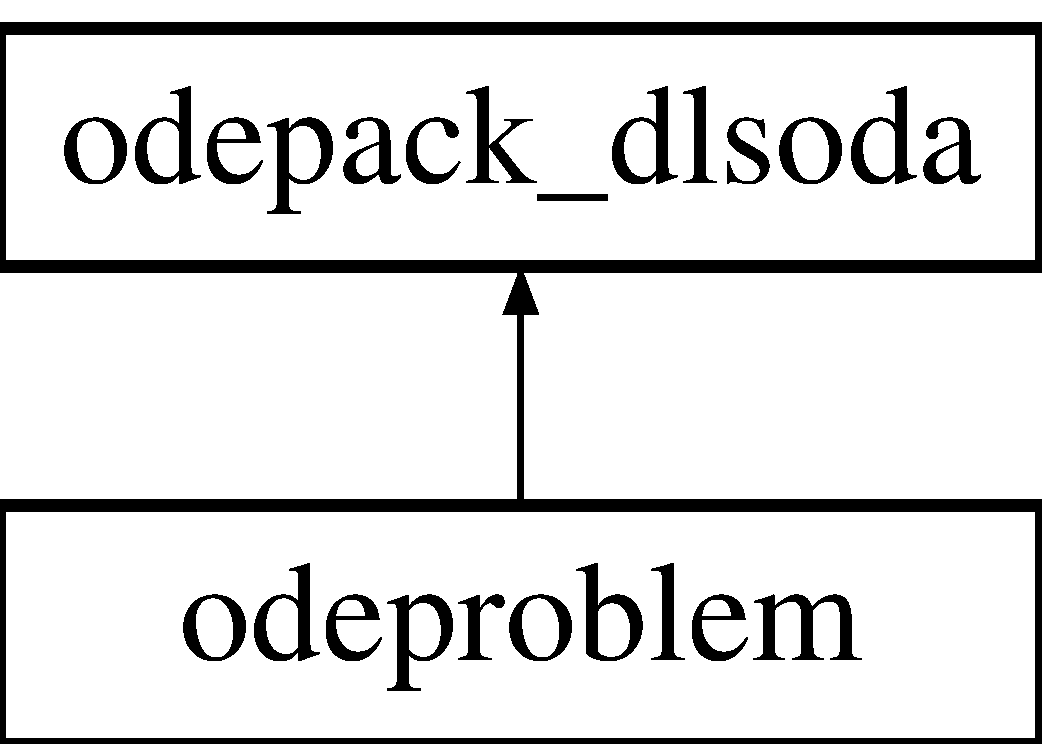
\includegraphics[height=2.000000cm]{classodepack__dlsoda}
\end{center}
\end{figure}
\subsection*{Public Member Functions}
\begin{DoxyCompactItemize}
\item 
\mbox{\Hypertarget{classodepack__dlsoda_a843b8ba43e2aff07daec1420cd25566d}\label{classodepack__dlsoda_a843b8ba43e2aff07daec1420cd25566d}} 
{\bfseries odepack\+\_\+dlsoda} (int npar\+\_\+, int neq\+\_\+)
\item 
\mbox{\Hypertarget{classodepack__dlsoda_ac9ff0de8a49daae6687347d37a57bc8b}\label{classodepack__dlsoda_ac9ff0de8a49daae6687347d37a57bc8b}} 
void {\bfseries hmax} (double value)
\item 
\mbox{\Hypertarget{classodepack__dlsoda_a65b0f71801ce0ddd2cae324907f685c3}\label{classodepack__dlsoda_a65b0f71801ce0ddd2cae324907f685c3}} 
void {\bfseries hmin} (double value)
\item 
\mbox{\Hypertarget{classodepack__dlsoda_a36703efaae208e98bc69f4c0f41f09e6}\label{classodepack__dlsoda_a36703efaae208e98bc69f4c0f41f09e6}} 
void {\bfseries ixpr} (int value)
\item 
\mbox{\Hypertarget{classodepack__dlsoda_a4a400ab24bfe3383c5875fd05a1c674a}\label{classodepack__dlsoda_a4a400ab24bfe3383c5875fd05a1c674a}} 
void {\bfseries maxsteps} (int value)
\item 
\mbox{\Hypertarget{classodepack__dlsoda_a6daa9e98e630de11df59019dc222c2d2}\label{classodepack__dlsoda_a6daa9e98e630de11df59019dc222c2d2}} 
void {\bfseries mxhnil} (int value)
\item 
\mbox{\Hypertarget{classodepack__dlsoda_ad22afd38954c315495f4111185081a5d}\label{classodepack__dlsoda_ad22afd38954c315495f4111185081a5d}} 
int {\bfseries istate} ()
\item 
\mbox{\Hypertarget{classodepack__dlsoda_a3d6e191ab00709e24bb478943065207d}\label{classodepack__dlsoda_a3d6e191ab00709e24bb478943065207d}} 
void {\bfseries istate} (int value)
\item 
\mbox{\Hypertarget{classodepack__dlsoda_a59bd524c172806073e20b056afcc5b2a}\label{classodepack__dlsoda_a59bd524c172806073e20b056afcc5b2a}} 
void {\bfseries lsoda\+\_\+init} ()
\item 
\mbox{\Hypertarget{classodepack__dlsoda_a157eeb6db451d1b882a2fbc4753dbccd}\label{classodepack__dlsoda_a157eeb6db451d1b882a2fbc4753dbccd}} 
int {\bfseries itask} ()
\item 
\mbox{\Hypertarget{classodepack__dlsoda_a345b08b1b6b65ee8e0736f8225ba9185}\label{classodepack__dlsoda_a345b08b1b6b65ee8e0736f8225ba9185}} 
void {\bfseries itask} (int itask)
\item 
\mbox{\Hypertarget{classodepack__dlsoda_a962ee79439a59f4cb41d94e95b7ba525}\label{classodepack__dlsoda_a962ee79439a59f4cb41d94e95b7ba525}} 
void {\bfseries tol} (double atol, double rtol)
\item 
\mbox{\Hypertarget{classodepack__dlsoda_a3b403151021e2e5766742f88c779ccf5}\label{classodepack__dlsoda_a3b403151021e2e5766742f88c779ccf5}} 
double $\ast$ {\bfseries rwork} ()
\item 
\mbox{\Hypertarget{classodepack__dlsoda_a0a5f8ba6ba0b8efd119189888eb29341}\label{classodepack__dlsoda_a0a5f8ba6ba0b8efd119189888eb29341}} 
void {\bfseries rwork} (int pos, double value)
\item 
\mbox{\Hypertarget{classodepack__dlsoda_a3b6fda49f4eb659a842215d6edb8fb4e}\label{classodepack__dlsoda_a3b6fda49f4eb659a842215d6edb8fb4e}} 
int $\ast$ {\bfseries iwork} ()
\item 
\mbox{\Hypertarget{classodepack__dlsoda_a173262fcf6a7d91c2efbc422fdcbee3a}\label{classodepack__dlsoda_a173262fcf6a7d91c2efbc422fdcbee3a}} 
void {\bfseries iwork} (int pos, int value)
\item 
\mbox{\Hypertarget{classodepack__dlsoda_a809c83e3b27e0ad742f08c18c62b72e2}\label{classodepack__dlsoda_a809c83e3b27e0ad742f08c18c62b72e2}} 
void {\bfseries tcrit} (double value)
\item 
\mbox{\Hypertarget{classodepack__dlsoda_ac213f89f6c310344d40d427a82712f01}\label{classodepack__dlsoda_ac213f89f6c310344d40d427a82712f01}} 
double $\ast$ {\bfseries y} ()
\item 
\mbox{\Hypertarget{classodepack__dlsoda_a7605648b51623b14733c9958df90494a}\label{classodepack__dlsoda_a7605648b51623b14733c9958df90494a}} 
void {\bfseries y} (const int pos, const double value)
\item 
\mbox{\Hypertarget{classodepack__dlsoda_afb0248bc488b07ac9fecbfd732b39e6e}\label{classodepack__dlsoda_afb0248bc488b07ac9fecbfd732b39e6e}} 
double {\bfseries y} (const int pos)
\item 
\mbox{\Hypertarget{classodepack__dlsoda_ad6b4e99f2e1aa37e7b2ecd876c79b2cf}\label{classodepack__dlsoda_ad6b4e99f2e1aa37e7b2ecd876c79b2cf}} 
double $\ast$ {\bfseries ydot} ()
\item 
\mbox{\Hypertarget{classodepack__dlsoda_a7626e417b46f44762cd167d836f3c461}\label{classodepack__dlsoda_a7626e417b46f44762cd167d836f3c461}} 
int {\bfseries npar} ()
\item 
\mbox{\Hypertarget{classodepack__dlsoda_a419a318700e6bac2163faac864c3e3d2}\label{classodepack__dlsoda_a419a318700e6bac2163faac864c3e3d2}} 
int {\bfseries neq} ()
\end{DoxyCompactItemize}
\subsection*{Protected Attributes}
\begin{DoxyCompactItemize}
\item 
\mbox{\Hypertarget{classodepack__dlsoda_a6c98ce6ec86aae4fea34ed04230bf0f8}\label{classodepack__dlsoda_a6c98ce6ec86aae4fea34ed04230bf0f8}} 
int \hyperlink{classodepack__dlsoda_a6c98ce6ec86aae4fea34ed04230bf0f8}{xliwork}
\begin{DoxyCompactList}\small\item\em length of iwork array \end{DoxyCompactList}\item 
\mbox{\Hypertarget{classodepack__dlsoda_a14a08a08073c9013bdac66a5addaac88}\label{classodepack__dlsoda_a14a08a08073c9013bdac66a5addaac88}} 
int \hyperlink{classodepack__dlsoda_a14a08a08073c9013bdac66a5addaac88}{xlrwork}
\begin{DoxyCompactList}\small\item\em length of rwork array \end{DoxyCompactList}\item 
\mbox{\Hypertarget{classodepack__dlsoda_a839d1d413392db48d73f8442d2a5f162}\label{classodepack__dlsoda_a839d1d413392db48d73f8442d2a5f162}} 
int \hyperlink{classodepack__dlsoda_a839d1d413392db48d73f8442d2a5f162}{xistate}
\begin{DoxyCompactList}\small\item\em istate value \end{DoxyCompactList}\item 
\mbox{\Hypertarget{classodepack__dlsoda_a169bda738ab8d3200068109d18ce6bbf}\label{classodepack__dlsoda_a169bda738ab8d3200068109d18ce6bbf}} 
int \hyperlink{classodepack__dlsoda_a169bda738ab8d3200068109d18ce6bbf}{xitask}
\begin{DoxyCompactList}\small\item\em itask value \end{DoxyCompactList}\item 
\mbox{\Hypertarget{classodepack__dlsoda_a4b57efab0a49bc331ef04d65f0da60bc}\label{classodepack__dlsoda_a4b57efab0a49bc331ef04d65f0da60bc}} 
int \hyperlink{classodepack__dlsoda_a4b57efab0a49bc331ef04d65f0da60bc}{xiopt}
\begin{DoxyCompactList}\small\item\em iopt value \end{DoxyCompactList}\item 
\mbox{\Hypertarget{classodepack__dlsoda_a731987a2a4da7215a053be9c33188732}\label{classodepack__dlsoda_a731987a2a4da7215a053be9c33188732}} 
int \hyperlink{classodepack__dlsoda_a731987a2a4da7215a053be9c33188732}{xitol}
\begin{DoxyCompactList}\small\item\em itol value \end{DoxyCompactList}\item 
\mbox{\Hypertarget{classodepack__dlsoda_accd405a79221a13138eb1055d8fdb4f4}\label{classodepack__dlsoda_accd405a79221a13138eb1055d8fdb4f4}} 
int \hyperlink{classodepack__dlsoda_accd405a79221a13138eb1055d8fdb4f4}{Neq}
\begin{DoxyCompactList}\small\item\em number of state variables \end{DoxyCompactList}\item 
\mbox{\Hypertarget{classodepack__dlsoda_a41b802250255bfbb9c7b3a0b0e3545c8}\label{classodepack__dlsoda_a41b802250255bfbb9c7b3a0b0e3545c8}} 
int \hyperlink{classodepack__dlsoda_a41b802250255bfbb9c7b3a0b0e3545c8}{Npar}
\begin{DoxyCompactList}\small\item\em number of model parameters \end{DoxyCompactList}\item 
\mbox{\Hypertarget{classodepack__dlsoda_a20ae2db2c2db96c2a084702f6b4290d4}\label{classodepack__dlsoda_a20ae2db2c2db96c2a084702f6b4290d4}} 
int \hyperlink{classodepack__dlsoda_a20ae2db2c2db96c2a084702f6b4290d4}{xjt}
\begin{DoxyCompactList}\small\item\em jacobian indicator \end{DoxyCompactList}\item 
\mbox{\Hypertarget{classodepack__dlsoda_a4d7b9b709e97aa1e5a37f5e405e300d3}\label{classodepack__dlsoda_a4d7b9b709e97aa1e5a37f5e405e300d3}} 
double \hyperlink{classodepack__dlsoda_a4d7b9b709e97aa1e5a37f5e405e300d3}{xatol}
\begin{DoxyCompactList}\small\item\em absolute tolerance \end{DoxyCompactList}\item 
\mbox{\Hypertarget{classodepack__dlsoda_a8e8b3aad24b1ab9ae0971bffba41b78a}\label{classodepack__dlsoda_a8e8b3aad24b1ab9ae0971bffba41b78a}} 
double \hyperlink{classodepack__dlsoda_a8e8b3aad24b1ab9ae0971bffba41b78a}{xrtol}
\begin{DoxyCompactList}\small\item\em relative tolerance \end{DoxyCompactList}\item 
\mbox{\Hypertarget{classodepack__dlsoda_a824cd623c15909783611cfc319ddbfb9}\label{classodepack__dlsoda_a824cd623c15909783611cfc319ddbfb9}} 
double $\ast$ \hyperlink{classodepack__dlsoda_a824cd623c15909783611cfc319ddbfb9}{xrwork}
\begin{DoxyCompactList}\small\item\em rwork array \end{DoxyCompactList}\item 
\mbox{\Hypertarget{classodepack__dlsoda_a111f730fd182cc30acea9327f5c224a1}\label{classodepack__dlsoda_a111f730fd182cc30acea9327f5c224a1}} 
int $\ast$ \hyperlink{classodepack__dlsoda_a111f730fd182cc30acea9327f5c224a1}{xiwork}
\begin{DoxyCompactList}\small\item\em iwork array \end{DoxyCompactList}\item 
\mbox{\Hypertarget{classodepack__dlsoda_a6dce361fe841a8a9f3d5d1400889627e}\label{classodepack__dlsoda_a6dce361fe841a8a9f3d5d1400889627e}} 
double $\ast$ \hyperlink{classodepack__dlsoda_a6dce361fe841a8a9f3d5d1400889627e}{Y}
\begin{DoxyCompactList}\small\item\em current value of state variables \end{DoxyCompactList}\item 
\mbox{\Hypertarget{classodepack__dlsoda_a3681231289f4223f080b460eb4cce7fc}\label{classodepack__dlsoda_a3681231289f4223f080b460eb4cce7fc}} 
double $\ast$ \hyperlink{classodepack__dlsoda_a3681231289f4223f080b460eb4cce7fc}{Ydot}
\begin{DoxyCompactList}\small\item\em current value of O\+D\+Es \end{DoxyCompactList}\end{DoxyCompactItemize}


The documentation for this class was generated from the following files\+:\begin{DoxyCompactItemize}
\item 
inst/include/\hyperlink{odepack__dlsoda_8h}{odepack\+\_\+dlsoda.\+h}\item 
src/\hyperlink{odepack__dlsoda_8cpp}{odepack\+\_\+dlsoda.\+cpp}\end{DoxyCompactItemize}

\hypertarget{classodeproblem}{}\section{odeproblem Class Reference}
\label{classodeproblem}\index{odeproblem@{odeproblem}}
Inheritance diagram for odeproblem\+:\begin{figure}[H]
\begin{center}
\leavevmode
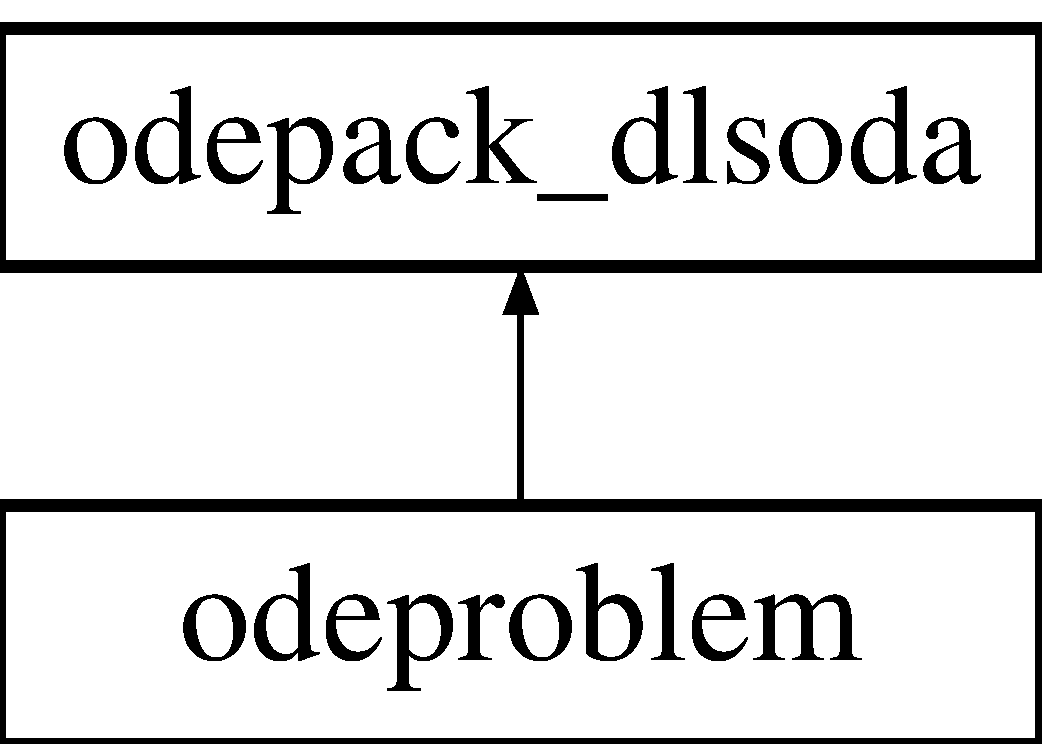
\includegraphics[height=2.000000cm]{classodeproblem}
\end{center}
\end{figure}
\subsection*{Public Member Functions}
\begin{DoxyCompactItemize}
\item 
\mbox{\Hypertarget{classodeproblem_acc18c1c3dfc77ab1191daffdd4382f14}\label{classodeproblem_acc18c1c3dfc77ab1191daffdd4382f14}} 
{\bfseries odeproblem} (Rcpp\+::\+Numeric\+Vector param, Rcpp\+::\+Numeric\+Vector init, Rcpp\+::\+List funs, int n\+\_\+capture\+\_\+)
\item 
virtual \hyperlink{classodeproblem_a00c35020fc03286fd4596f25b3d82e34}{$\sim$odeproblem} ()
\begin{DoxyCompactList}\small\item\em Destructor for odeproblem object. \end{DoxyCompactList}\item 
\mbox{\Hypertarget{classodeproblem_a0d35904cd64604463cba0065a3fc9c01}\label{classodeproblem_a0d35904cd64604463cba0065a3fc9c01}} 
void {\bfseries advance} (double tfrom, double tto)
\item 
\mbox{\Hypertarget{classodeproblem_a3846fa84421ca3e2f84eceaf2958c519}\label{classodeproblem_a3846fa84421ca3e2f84eceaf2958c519}} 
void {\bfseries call\+\_\+derivs} (int $\ast$neq, double $\ast$t, double $\ast$y, double $\ast$ydot)
\item 
\mbox{\Hypertarget{classodeproblem_a2de806c10c0ce7e2a422b9d4210640f9}\label{classodeproblem_a2de806c10c0ce7e2a422b9d4210640f9}} 
void {\bfseries init} (int pos, double value)
\item 
\mbox{\Hypertarget{classodeproblem_a1c53a46511e8c1739e4132073304c5e7}\label{classodeproblem_a1c53a46511e8c1739e4132073304c5e7}} 
double {\bfseries init} (int pos)
\item 
void \hyperlink{classodeproblem_a415e0001bfe1282764c339b6e8695ab8}{init\+\_\+call} (const double \&time)
\item 
void \hyperlink{classodeproblem_adc4a5dbcc9561903a7aa81a90e8a908b}{init\+\_\+call\+\_\+record} (const double \&time)
\item 
void \hyperlink{classodeproblem_a258d7fdca6eb1b49cac25cea9fcca9c4}{y\+\_\+init} (int pos, double value)
\item 
\mbox{\Hypertarget{classodeproblem_a21fec9644d1f590e11fc80cd50ff5f5c}\label{classodeproblem_a21fec9644d1f590e11fc80cd50ff5f5c}} 
void {\bfseries y\+\_\+init} (Rcpp\+::\+Numeric\+Vector x)
\item 
\mbox{\Hypertarget{classodeproblem_aeb23afacc04444d129c91746e003240a}\label{classodeproblem_aeb23afacc04444d129c91746e003240a}} 
void \hyperlink{classodeproblem_aeb23afacc04444d129c91746e003240a}{y\+\_\+add} (const unsigned int pos, const double \&value)
\begin{DoxyCompactList}\small\item\em add {\ttfamily value} to compartment {\ttfamily pos} \end{DoxyCompactList}\item 
\mbox{\Hypertarget{classodeproblem_a62371ab3a7331c680da61c34e0a77390}\label{classodeproblem_a62371ab3a7331c680da61c34e0a77390}} 
void \hyperlink{classodeproblem_a62371ab3a7331c680da61c34e0a77390}{table\+\_\+call} ()
\begin{DoxyCompactList}\small\item\em Call {\ttfamily \$\+T\+A\+B\+LE} function. \end{DoxyCompactList}\item 
\mbox{\Hypertarget{classodeproblem_a5671e548c6e81afd353a45b4b3c845af}\label{classodeproblem_a5671e548c6e81afd353a45b4b3c845af}} 
void {\bfseries table\+\_\+init\+\_\+call} ()
\item 
\mbox{\Hypertarget{classodeproblem_a23ba805e57f18ec631645247c631c0ac}\label{classodeproblem_a23ba805e57f18ec631645247c631c0ac}} 
void \hyperlink{classodeproblem_a23ba805e57f18ec631645247c631c0ac}{config\+\_\+call} ()
\begin{DoxyCompactList}\small\item\em Call {\ttfamily \$\+P\+R\+E\+A\+M\+B\+LE} function. \end{DoxyCompactList}\item 
\mbox{\Hypertarget{classodeproblem_a40b09d94a66b474fd65213e415ddc969}\label{classodeproblem_a40b09d94a66b474fd65213e415ddc969}} 
void {\bfseries set\+\_\+d} (rec\+\_\+ptr this\+\_\+rec)
\item 
\mbox{\Hypertarget{classodeproblem_a7d4724eff5756cd90aa4d8d7571b932e}\label{classodeproblem_a7d4724eff5756cd90aa4d8d7571b932e}} 
void {\bfseries omega} (Rcpp\+::\+Numeric\+Matrix \&x)
\item 
\mbox{\Hypertarget{classodeproblem_abb8cdbe6d433204cb209405789b521f8}\label{classodeproblem_abb8cdbe6d433204cb209405789b521f8}} 
void {\bfseries sigma} (Rcpp\+::\+Numeric\+Matrix \&x)
\item 
\mbox{\Hypertarget{classodeproblem_a2827c3ef1ce3acaa967dd6e315debfe3}\label{classodeproblem_a2827c3ef1ce3acaa967dd6e315debfe3}} 
arma\+::mat {\bfseries mv\+\_\+omega} (int n)
\item 
\mbox{\Hypertarget{classodeproblem_aa7d69c4024cf6783ce7c2556367a0675}\label{classodeproblem_aa7d69c4024cf6783ce7c2556367a0675}} 
arma\+::mat {\bfseries mv\+\_\+sigma} (int n)
\item 
\mbox{\Hypertarget{classodeproblem_a6a1253090d65c34a9a26e77b01a82573}\label{classodeproblem_a6a1253090d65c34a9a26e77b01a82573}} 
void {\bfseries pass\+\_\+envir} (Rcpp\+::\+Environment $\ast$x)
\item 
\mbox{\Hypertarget{classodeproblem_a962ce2e5ac9d9b6514e6d06c52ece74e}\label{classodeproblem_a962ce2e5ac9d9b6514e6d06c52ece74e}} 
bool {\bfseries C\+F\+O\+N\+S\+T\+OP} ()
\item 
\mbox{\Hypertarget{classodeproblem_aeedc05b398a0440b9d8f96876e56a8a6}\label{classodeproblem_aeedc05b398a0440b9d8f96876e56a8a6}} 
const double $\ast$ {\bfseries param} () const
\item 
\mbox{\Hypertarget{classodeproblem_a9669835dd93ca8415466b031aaccf0a5}\label{classodeproblem_a9669835dd93ca8415466b031aaccf0a5}} 
void {\bfseries param} (int pos, double value)
\item 
\mbox{\Hypertarget{classodeproblem_af6e95b3ef6e66fd90bd74d9d3e4cfdb9}\label{classodeproblem_af6e95b3ef6e66fd90bd74d9d3e4cfdb9}} 
void {\bfseries rate} (unsigned int pos, double value)
\item 
\mbox{\Hypertarget{classodeproblem_abb46c0c4c4ba37273775f207989b8593}\label{classodeproblem_abb46c0c4c4ba37273775f207989b8593}} 
double {\bfseries rate} (unsigned int pos)
\item 
\mbox{\Hypertarget{classodeproblem_a037f4a9a3c152237557d092f5c9b18f2}\label{classodeproblem_a037f4a9a3c152237557d092f5c9b18f2}} 
void {\bfseries rate0} (unsigned int pos, double value)
\item 
\mbox{\Hypertarget{classodeproblem_a1a26afe1439b4b827e346a1eec4d5284}\label{classodeproblem_a1a26afe1439b4b827e346a1eec4d5284}} 
double {\bfseries rate0} (unsigned int pos)
\item 
\mbox{\Hypertarget{classodeproblem_a7b5b4b266d8205069f6fa806fec959bd}\label{classodeproblem_a7b5b4b266d8205069f6fa806fec959bd}} 
int {\bfseries rate\+\_\+count} (unsigned int pos)
\item 
\mbox{\Hypertarget{classodeproblem_a7985d0d2c71f3210fa043038efa7696b}\label{classodeproblem_a7985d0d2c71f3210fa043038efa7696b}} 
void {\bfseries rate\+\_\+add} (unsigned int pos, const double \&value)
\item 
\mbox{\Hypertarget{classodeproblem_a6cd2af7fdeca1734d4ac96c31286b086}\label{classodeproblem_a6cd2af7fdeca1734d4ac96c31286b086}} 
void {\bfseries rate\+\_\+rm} (unsigned int pos, const double \&value)
\item 
\mbox{\Hypertarget{classodeproblem_aec484a1e3327cac5360e9b323ce995f6}\label{classodeproblem_aec484a1e3327cac5360e9b323ce995f6}} 
void {\bfseries rate\+\_\+bump} (const unsigned int pos, const double \&value)
\item 
\mbox{\Hypertarget{classodeproblem_a89919c8495a969c85027b645cc611549}\label{classodeproblem_a89919c8495a969c85027b645cc611549}} 
void \hyperlink{classodeproblem_a89919c8495a969c85027b645cc611549}{rate\+\_\+reset} ()
\begin{DoxyCompactList}\small\item\em Reset all infusion rates. \end{DoxyCompactList}\item 
\mbox{\Hypertarget{classodeproblem_a6b01a064fdeca43c8d70c9acaf4cd01a}\label{classodeproblem_a6b01a064fdeca43c8d70c9acaf4cd01a}} 
void {\bfseries dur} (unsigned int pos, double value)
\item 
\mbox{\Hypertarget{classodeproblem_aa55e249b79cee0dd7292e2e26c512d4d}\label{classodeproblem_aa55e249b79cee0dd7292e2e26c512d4d}} 
double {\bfseries dur} (unsigned int pos)
\item 
\mbox{\Hypertarget{classodeproblem_ae7047dc9fe7335cb4367a90a945801b5}\label{classodeproblem_ae7047dc9fe7335cb4367a90a945801b5}} 
void {\bfseries fbio} (unsigned int pos, double value)
\item 
\mbox{\Hypertarget{classodeproblem_abe453ef912e890b1f6e1fea51e627a5e}\label{classodeproblem_abe453ef912e890b1f6e1fea51e627a5e}} 
double {\bfseries fbio} (unsigned int pos)
\item 
\mbox{\Hypertarget{classodeproblem_a486c40b4b6746afe3aa079cb7bb5c7dc}\label{classodeproblem_a486c40b4b6746afe3aa079cb7bb5c7dc}} 
double {\bfseries alag} (int cmt)
\item 
\mbox{\Hypertarget{classodeproblem_ae210665b2d2c52c802aa2d95304ba111}\label{classodeproblem_ae210665b2d2c52c802aa2d95304ba111}} 
void \hyperlink{classodeproblem_ae210665b2d2c52c802aa2d95304ba111}{reset\+\_\+newid} (const double id\+\_\+)
\begin{DoxyCompactList}\small\item\em Reset {\ttfamily odeproblem} object for new individual. \end{DoxyCompactList}\item 
\mbox{\Hypertarget{classodeproblem_a54f096ed754117bfe2c1a58d6661c69c}\label{classodeproblem_a54f096ed754117bfe2c1a58d6661c69c}} 
void {\bfseries eta} (int pos, double value)
\item 
\mbox{\Hypertarget{classodeproblem_a21f796445e785d46939ac4c50e719c37}\label{classodeproblem_a21f796445e785d46939ac4c50e719c37}} 
void {\bfseries eps} (int pos, double value)
\item 
\mbox{\Hypertarget{classodeproblem_ab23130b9de7b9b8af0f72a01d1168a87}\label{classodeproblem_ab23130b9de7b9b8af0f72a01d1168a87}} 
bool {\bfseries systemoff} ()
\item 
\mbox{\Hypertarget{classodeproblem_a2b6729af8ce989fe14c54657ae7c59f1}\label{classodeproblem_a2b6729af8ce989fe14c54657ae7c59f1}} 
void {\bfseries on} (unsigned short int cmt)
\item 
\mbox{\Hypertarget{classodeproblem_a0f76cc6a34e82e34edc6c68c390bddae}\label{classodeproblem_a0f76cc6a34e82e34edc6c68c390bddae}} 
void {\bfseries off} (unsigned short int cmt)
\item 
\mbox{\Hypertarget{classodeproblem_afa433b145c17640cbcf31e6a72e009f6}\label{classodeproblem_afa433b145c17640cbcf31e6a72e009f6}} 
int {\bfseries is\+\_\+on} (unsigned int eq\+\_\+n)
\item 
\mbox{\Hypertarget{classodeproblem_a570f475a1f81d2128fa90b9551ec9c37}\label{classodeproblem_a570f475a1f81d2128fa90b9551ec9c37}} 
void {\bfseries time} (double time\+\_\+)
\item 
\mbox{\Hypertarget{classodeproblem_a370c76cd4b8ae3ebd2d9ce3b1dd6a013}\label{classodeproblem_a370c76cd4b8ae3ebd2d9ce3b1dd6a013}} 
void {\bfseries newind} (unsigned int newind\+\_\+)
\item 
\mbox{\Hypertarget{classodeproblem_a352d6631fea50cfe328011c6c337e8d7}\label{classodeproblem_a352d6631fea50cfe328011c6c337e8d7}} 
unsigned int {\bfseries newind} ()
\item 
\mbox{\Hypertarget{classodeproblem_a01838d1e6b48e01746eea68d4f1603a2}\label{classodeproblem_a01838d1e6b48e01746eea68d4f1603a2}} 
void {\bfseries advan} (int x)
\item 
\mbox{\Hypertarget{classodeproblem_a07c37e014e44c8cb933701870ca7f639}\label{classodeproblem_a07c37e014e44c8cb933701870ca7f639}} 
int {\bfseries advan} ()
\item 
\mbox{\Hypertarget{classodeproblem_a197d9523fe129bb7e35e4e20c8e09fc2}\label{classodeproblem_a197d9523fe129bb7e35e4e20c8e09fc2}} 
void {\bfseries advan2} (const double \&tfrom, const double \&tto)
\item 
\mbox{\Hypertarget{classodeproblem_a9e2b9f80bd614d5a03109e75e1fde18b}\label{classodeproblem_a9e2b9f80bd614d5a03109e75e1fde18b}} 
void {\bfseries advan4} (const double \&tfrom, const double \&tto)
\item 
\mbox{\Hypertarget{classodeproblem_a96c6c7170fe10ea41cd889e5ff0a4dcd}\label{classodeproblem_a96c6c7170fe10ea41cd889e5ff0a4dcd}} 
void \hyperlink{classodeproblem_a96c6c7170fe10ea41cd889e5ff0a4dcd}{neta} (int n)
\begin{DoxyCompactList}\small\item\em set number of {\ttfamily E\+T\+As} in the model \end{DoxyCompactList}\item 
\mbox{\Hypertarget{classodeproblem_a99d73608dddbb8fdaa58592bda59d45a}\label{classodeproblem_a99d73608dddbb8fdaa58592bda59d45a}} 
void \hyperlink{classodeproblem_a99d73608dddbb8fdaa58592bda59d45a}{neps} (int n)
\begin{DoxyCompactList}\small\item\em set number of {\ttfamily E\+P\+Ss} in the model \end{DoxyCompactList}\item 
\mbox{\Hypertarget{classodeproblem_ad7800dc80fb646deea76e440af5fa6c6}\label{classodeproblem_ad7800dc80fb646deea76e440af5fa6c6}} 
void {\bfseries nid} (int n)
\item 
\mbox{\Hypertarget{classodeproblem_ae02303871f68a48c256ccc7ce2c71981}\label{classodeproblem_ae02303871f68a48c256ccc7ce2c71981}} 
void {\bfseries nrow} (int n)
\item 
\mbox{\Hypertarget{classodeproblem_ada58c0594a72e21a3aa3c56876599df4}\label{classodeproblem_ada58c0594a72e21a3aa3c56876599df4}} 
void {\bfseries idn} (int n)
\item 
\mbox{\Hypertarget{classodeproblem_ad385d5c62a5a215b537cbd88a98e4d28}\label{classodeproblem_ad385d5c62a5a215b537cbd88a98e4d28}} 
void {\bfseries rown} (int n)
\item 
\mbox{\Hypertarget{classodeproblem_a5ae9d2f4c7b37407ddeddfdbcae7590c}\label{classodeproblem_a5ae9d2f4c7b37407ddeddfdbcae7590c}} 
\hyperlink{mrgsolv_8h_ac6aa1a2351760492203846ae74778c05}{dvec} \& {\bfseries mtime} ()
\item 
\mbox{\Hypertarget{classodeproblem_a54adaa665b551ba6ffe835e2d2ddf48f}\label{classodeproblem_a54adaa665b551ba6ffe835e2d2ddf48f}} 
\hyperlink{mrgsolv_8h_ac6aa1a2351760492203846ae74778c05}{dvec} \& {\bfseries get\+\_\+capture} ()
\item 
\mbox{\Hypertarget{classodeproblem_a9a053ea59d585643d52825c31e9ed203}\label{classodeproblem_a9a053ea59d585643d52825c31e9ed203}} 
double {\bfseries capture} (int i)
\item 
\mbox{\Hypertarget{classodeproblem_a0058d8ce64adbefd960571d19de47ca4}\label{classodeproblem_a0058d8ce64adbefd960571d19de47ca4}} 
void {\bfseries copy\+\_\+parin} (const Rcpp\+::\+List \&parin)
\item 
\mbox{\Hypertarget{classodeproblem_a44cc384c4d3c6e9c95dbafdfc92ba7b6}\label{classodeproblem_a44cc384c4d3c6e9c95dbafdfc92ba7b6}} 
void {\bfseries copy\+\_\+funs} (const Rcpp\+::\+List \&funs)
\end{DoxyCompactItemize}
\subsection*{Protected Attributes}
\begin{DoxyCompactItemize}
\item 
\mbox{\Hypertarget{classodeproblem_a8d6506f6a9e0676911ee86659db725ae}\label{classodeproblem_a8d6506f6a9e0676911ee86659db725ae}} 
double $\ast$ \hyperlink{classodeproblem_a8d6506f6a9e0676911ee86659db725ae}{Param}
\begin{DoxyCompactList}\small\item\em model parameters \end{DoxyCompactList}\item 
\mbox{\Hypertarget{classodeproblem_ae467cabc47b5d75c07cb2d48915d4507}\label{classodeproblem_ae467cabc47b5d75c07cb2d48915d4507}} 
\hyperlink{mrgsolv_8h_ac6aa1a2351760492203846ae74778c05}{dvec} \hyperlink{classodeproblem_ae467cabc47b5d75c07cb2d48915d4507}{R0}
\begin{DoxyCompactList}\small\item\em acutal current infusion rate \end{DoxyCompactList}\item 
\mbox{\Hypertarget{classodeproblem_a51662bd0cd437b3481f83b662172d505}\label{classodeproblem_a51662bd0cd437b3481f83b662172d505}} 
std\+::vector$<$ unsigned int $>$ \hyperlink{classodeproblem_a51662bd0cd437b3481f83b662172d505}{infusion\+\_\+count}
\begin{DoxyCompactList}\small\item\em number of active infusions \end{DoxyCompactList}\item 
\mbox{\Hypertarget{classodeproblem_af0b19177db1bdd5a610b34c298b8a7e5}\label{classodeproblem_af0b19177db1bdd5a610b34c298b8a7e5}} 
\hyperlink{mrgsolv_8h_ac6aa1a2351760492203846ae74778c05}{dvec} \hyperlink{classodeproblem_af0b19177db1bdd5a610b34c298b8a7e5}{R}
\begin{DoxyCompactList}\small\item\em receive user input for infusion rate \end{DoxyCompactList}\item 
\mbox{\Hypertarget{classodeproblem_af46382c0b9a5a489f726d0fb360d9e40}\label{classodeproblem_af46382c0b9a5a489f726d0fb360d9e40}} 
\hyperlink{mrgsolv_8h_ac6aa1a2351760492203846ae74778c05}{dvec} \hyperlink{classodeproblem_af46382c0b9a5a489f726d0fb360d9e40}{D}
\begin{DoxyCompactList}\small\item\em receive user input for infusion duration \end{DoxyCompactList}\item 
\mbox{\Hypertarget{classodeproblem_a32596188c9d34831dd386240953691c4}\label{classodeproblem_a32596188c9d34831dd386240953691c4}} 
\hyperlink{mrgsolv_8h_ac6aa1a2351760492203846ae74778c05}{dvec} \hyperlink{classodeproblem_a32596188c9d34831dd386240953691c4}{Init\+\_\+value}
\begin{DoxyCompactList}\small\item\em initial conditions \end{DoxyCompactList}\item 
\mbox{\Hypertarget{classodeproblem_ab085f5070edbc99c01c55513ed74bdb6}\label{classodeproblem_ab085f5070edbc99c01c55513ed74bdb6}} 
\hyperlink{mrgsolv_8h_ac6aa1a2351760492203846ae74778c05}{dvec} \hyperlink{classodeproblem_ab085f5070edbc99c01c55513ed74bdb6}{Init\+\_\+dummy}
\begin{DoxyCompactList}\small\item\em initial conditions for user input \end{DoxyCompactList}\item 
\mbox{\Hypertarget{classodeproblem_a5443840315f48d9d1d9843cac27e80d9}\label{classodeproblem_a5443840315f48d9d1d9843cac27e80d9}} 
\hyperlink{mrgsolv_8h_ac6aa1a2351760492203846ae74778c05}{dvec} \hyperlink{classodeproblem_a5443840315f48d9d1d9843cac27e80d9}{F}
\begin{DoxyCompactList}\small\item\em bioavability \end{DoxyCompactList}\item 
\mbox{\Hypertarget{classodeproblem_a6148fd047b80b6c33a5f2468c3b134af}\label{classodeproblem_a6148fd047b80b6c33a5f2468c3b134af}} 
\hyperlink{mrgsolv_8h_ac6aa1a2351760492203846ae74778c05}{dvec} \hyperlink{classodeproblem_a6148fd047b80b6c33a5f2468c3b134af}{Alag}
\begin{DoxyCompactList}\small\item\em dosing lag time \end{DoxyCompactList}\item 
\mbox{\Hypertarget{classodeproblem_afa0a937e8489a0249ad57a34d9b802a5}\label{classodeproblem_afa0a937e8489a0249ad57a34d9b802a5}} 
\hyperlink{odeproblem_8h_a9865ab8bde33af2df4bccee47db6d44a}{deriv\+\_\+func} $\ast$ \hyperlink{classodeproblem_afa0a937e8489a0249ad57a34d9b802a5}{Derivs}
\begin{DoxyCompactList}\small\item\em {\ttfamily \$\+O\+DE} function \end{DoxyCompactList}\item 
\mbox{\Hypertarget{classodeproblem_a4d0e7e54edac6020951cc005b3d529ec}\label{classodeproblem_a4d0e7e54edac6020951cc005b3d529ec}} 
\hyperlink{odeproblem_8h_a6192c201d632b8498cc03adf5a28e309}{init\+\_\+func} $\ast$ \hyperlink{classodeproblem_a4d0e7e54edac6020951cc005b3d529ec}{Inits}
\begin{DoxyCompactList}\small\item\em {\ttfamily \$\+M\+A\+IN} function \end{DoxyCompactList}\item 
\mbox{\Hypertarget{classodeproblem_ac117624df1306eb9cdbd92207c78afe7}\label{classodeproblem_ac117624df1306eb9cdbd92207c78afe7}} 
\hyperlink{odeproblem_8h_a283822b36ffc7e50e9ed7e28ac3d261c}{table\+\_\+func} $\ast$ \hyperlink{classodeproblem_ac117624df1306eb9cdbd92207c78afe7}{Table}
\begin{DoxyCompactList}\small\item\em {\ttfamily \$\+T\+A\+B\+LE} function \end{DoxyCompactList}\item 
\mbox{\Hypertarget{classodeproblem_a9a44457570e8d3358a0b41903a78e592}\label{classodeproblem_a9a44457570e8d3358a0b41903a78e592}} 
\hyperlink{odeproblem_8h_ab0c5ef95f66e5b23dc7868228e3a5900}{config\+\_\+func} $\ast$ \hyperlink{classodeproblem_a9a44457570e8d3358a0b41903a78e592}{Config}
\begin{DoxyCompactList}\small\item\em {\ttfamily \$\+P\+R\+E\+A\+M\+B\+LE} function \end{DoxyCompactList}\item 
\mbox{\Hypertarget{classodeproblem_a205d9c5f24a66739716e3d4db3382043}\label{classodeproblem_a205d9c5f24a66739716e3d4db3382043}} 
std\+::vector$<$ int $>$ \hyperlink{classodeproblem_a205d9c5f24a66739716e3d4db3382043}{On}
\begin{DoxyCompactList}\small\item\em compartment on/off indicator \end{DoxyCompactList}\item 
\mbox{\Hypertarget{classodeproblem_a950b8464c187a2b46fa6bfaa2052ff85}\label{classodeproblem_a950b8464c187a2b46fa6bfaa2052ff85}} 
\hyperlink{structdatabox}{databox} \hyperlink{classodeproblem_a950b8464c187a2b46fa6bfaa2052ff85}{d}
\begin{DoxyCompactList}\small\item\em various data passed to model functions \end{DoxyCompactList}\item 
\mbox{\Hypertarget{classodeproblem_a03f5d0954b46554399ff09ee131f9071}\label{classodeproblem_a03f5d0954b46554399ff09ee131f9071}} 
int \hyperlink{classodeproblem_a03f5d0954b46554399ff09ee131f9071}{Advan}
\begin{DoxyCompactList}\small\item\em simulation mode\+: 1/2/3/4 (PK models) or 13 (odes) \end{DoxyCompactList}\item 
\mbox{\Hypertarget{classodeproblem_a2e097ea96af2c293904053e764e63263}\label{classodeproblem_a2e097ea96af2c293904053e764e63263}} 
\hyperlink{mrgsolv_8h_ac6aa1a2351760492203846ae74778c05}{dvec} \hyperlink{classodeproblem_a2e097ea96af2c293904053e764e63263}{a}
\begin{DoxyCompactList}\small\item\em used for advan 1/2/3/4 calculations \end{DoxyCompactList}\item 
\mbox{\Hypertarget{classodeproblem_a2cc33c6e54bfecab2128965d712f4ddf}\label{classodeproblem_a2cc33c6e54bfecab2128965d712f4ddf}} 
\hyperlink{mrgsolv_8h_ac6aa1a2351760492203846ae74778c05}{dvec} \hyperlink{classodeproblem_a2cc33c6e54bfecab2128965d712f4ddf}{alpha}
\begin{DoxyCompactList}\small\item\em used for advan 1/2/3/4 calculation \end{DoxyCompactList}\item 
\mbox{\Hypertarget{classodeproblem_a4f2c3157beb52a27c029b4cb7bb8d7e5}\label{classodeproblem_a4f2c3157beb52a27c029b4cb7bb8d7e5}} 
\hyperlink{structresim}{resim} \hyperlink{classodeproblem_a4f2c3157beb52a27c029b4cb7bb8d7e5}{simeta}
\begin{DoxyCompactList}\small\item\em functor for resimulating etas \end{DoxyCompactList}\item 
\mbox{\Hypertarget{classodeproblem_a312484a436a3bb0ea55276fa97d23fb5}\label{classodeproblem_a312484a436a3bb0ea55276fa97d23fb5}} 
\hyperlink{structresim}{resim} \hyperlink{classodeproblem_a312484a436a3bb0ea55276fa97d23fb5}{simeps}
\begin{DoxyCompactList}\small\item\em functor for resimulating epsilons \end{DoxyCompactList}\item 
\mbox{\Hypertarget{classodeproblem_a38b999143a87c562d9db57e5fb82aa83}\label{classodeproblem_a38b999143a87c562d9db57e5fb82aa83}} 
arma\+::mat \hyperlink{classodeproblem_a38b999143a87c562d9db57e5fb82aa83}{Omega}
\begin{DoxyCompactList}\small\item\em variance/covariance matrix for between-\/subject variability \end{DoxyCompactList}\item 
\mbox{\Hypertarget{classodeproblem_ada2a77ef3f99c53d24e64026f356b99d}\label{classodeproblem_ada2a77ef3f99c53d24e64026f356b99d}} 
arma\+::mat \hyperlink{classodeproblem_ada2a77ef3f99c53d24e64026f356b99d}{Sigma}
\begin{DoxyCompactList}\small\item\em variance/covariance matrix for within-\/subject variability \end{DoxyCompactList}\item 
\mbox{\Hypertarget{classodeproblem_a2f93a3e1c10c2d1bba1a359bb3321cc0}\label{classodeproblem_a2f93a3e1c10c2d1bba1a359bb3321cc0}} 
\hyperlink{mrgsolv_8h_ac6aa1a2351760492203846ae74778c05}{dvec} \hyperlink{classodeproblem_a2f93a3e1c10c2d1bba1a359bb3321cc0}{pred}
\begin{DoxyCompactList}\small\item\em brings clearances, volumes, and kas for advan 1/2/3/4 calculations \end{DoxyCompactList}\item 
\mbox{\Hypertarget{classodeproblem_a4244e3ca9e9d52598d776c45fbb18ca4}\label{classodeproblem_a4244e3ca9e9d52598d776c45fbb18ca4}} 
\hyperlink{mrgsolv_8h_ac6aa1a2351760492203846ae74778c05}{dvec} \hyperlink{classodeproblem_a4244e3ca9e9d52598d776c45fbb18ca4}{Capture}
\begin{DoxyCompactList}\small\item\em captured data items \end{DoxyCompactList}\end{DoxyCompactItemize}


\subsection{Constructor \& Destructor Documentation}
\mbox{\Hypertarget{classodeproblem_a00c35020fc03286fd4596f25b3d82e34}\label{classodeproblem_a00c35020fc03286fd4596f25b3d82e34}} 
\index{odeproblem@{odeproblem}!````~odeproblem@{$\sim$odeproblem}}
\index{````~odeproblem@{$\sim$odeproblem}!odeproblem@{odeproblem}}
\subsubsection{\texorpdfstring{$\sim$odeproblem()}{~odeproblem()}}
{\footnotesize\ttfamily odeproblem\+::$\sim$odeproblem (\begin{DoxyParamCaption}{ }\end{DoxyParamCaption})\hspace{0.3cm}{\ttfamily [virtual]}}



Destructor for odeproblem object. 

Upon object construction, odeproblem dynamically allocates the Param array. 

\subsection{Member Function Documentation}
\mbox{\Hypertarget{classodeproblem_a415e0001bfe1282764c339b6e8695ab8}\label{classodeproblem_a415e0001bfe1282764c339b6e8695ab8}} 
\index{odeproblem@{odeproblem}!init\+\_\+call@{init\+\_\+call}}
\index{init\+\_\+call@{init\+\_\+call}!odeproblem@{odeproblem}}
\subsubsection{\texorpdfstring{init\+\_\+call()}{init\_call()}}
{\footnotesize\ttfamily void odeproblem\+::init\+\_\+call (\begin{DoxyParamCaption}\item[{const double \&}]{time }\end{DoxyParamCaption})}

Call {\ttfamily \$\+M\+A\+IN} to get the initial conditions.


\begin{DoxyParams}{Parameters}
{\em time} & the time to assume for the calculation \\
\hline
\end{DoxyParams}
\mbox{\Hypertarget{classodeproblem_adc4a5dbcc9561903a7aa81a90e8a908b}\label{classodeproblem_adc4a5dbcc9561903a7aa81a90e8a908b}} 
\index{odeproblem@{odeproblem}!init\+\_\+call\+\_\+record@{init\+\_\+call\+\_\+record}}
\index{init\+\_\+call\+\_\+record@{init\+\_\+call\+\_\+record}!odeproblem@{odeproblem}}
\subsubsection{\texorpdfstring{init\+\_\+call\+\_\+record()}{init\_call\_record()}}
{\footnotesize\ttfamily void odeproblem\+::init\+\_\+call\+\_\+record (\begin{DoxyParamCaption}\item[{const double \&}]{time }\end{DoxyParamCaption})}

Call {\ttfamily \$\+M\+A\+IN} with the dummy initial condition vector.


\begin{DoxyParams}{Parameters}
{\em time} & the time to assume when making the call. \\
\hline
\end{DoxyParams}
\mbox{\Hypertarget{classodeproblem_a258d7fdca6eb1b49cac25cea9fcca9c4}\label{classodeproblem_a258d7fdca6eb1b49cac25cea9fcca9c4}} 
\index{odeproblem@{odeproblem}!y\+\_\+init@{y\+\_\+init}}
\index{y\+\_\+init@{y\+\_\+init}!odeproblem@{odeproblem}}
\subsubsection{\texorpdfstring{y\+\_\+init()}{y\_init()}}
{\footnotesize\ttfamily void odeproblem\+::y\+\_\+init (\begin{DoxyParamCaption}\item[{int}]{pos,  }\item[{double}]{value }\end{DoxyParamCaption})}

Assigns values to both the compartment and the vector of initial conditions.


\begin{DoxyParams}{Parameters}
{\em pos} & the compartment number (C++ indexing) \\
\hline
{\em value} & the value for the compartment \\
\hline
\end{DoxyParams}


The documentation for this class was generated from the following files\+:\begin{DoxyCompactItemize}
\item 
inst/include/\hyperlink{odeproblem_8h}{odeproblem.\+h}\item 
src/\hyperlink{odeproblem_8cpp}{odeproblem.\+cpp}\end{DoxyCompactItemize}

\hypertarget{structresim}{}\section{resim Struct Reference}
\label{structresim}\index{resim@{resim}}


Resim functor.  




{\ttfamily \#include $<$mrgsolv.\+h$>$}

\subsection*{Public Member Functions}
\begin{DoxyCompactItemize}
\item 
\mbox{\Hypertarget{structresim_a8776836c59a5748e28d68d795569064b}\label{structresim_a8776836c59a5748e28d68d795569064b}} 
\hyperlink{structresim_a8776836c59a5748e28d68d795569064b}{resim} (refun $\ast$x, void $\ast$y)
\begin{DoxyCompactList}\small\item\em resim constructor \end{DoxyCompactList}\item 
\mbox{\Hypertarget{structresim_a66f6218d872d52eab1b2f7560f2c1b72}\label{structresim_a66f6218d872d52eab1b2f7560f2c1b72}} 
void {\bfseries operator()} ()
\end{DoxyCompactItemize}
\subsection*{Protected Attributes}
\begin{DoxyCompactItemize}
\item 
\mbox{\Hypertarget{structresim_a34ecef977366860be72ee4c1a8ee2ba6}\label{structresim_a34ecef977366860be72ee4c1a8ee2ba6}} 
refun $\ast$ \hyperlink{structresim_a34ecef977366860be72ee4c1a8ee2ba6}{fun}
\begin{DoxyCompactList}\small\item\em function to call to re-\/simulate \end{DoxyCompactList}\item 
\mbox{\Hypertarget{structresim_a85a513d872c25a973fafa56d4453c4e9}\label{structresim_a85a513d872c25a973fafa56d4453c4e9}} 
void $\ast$ \hyperlink{structresim_a85a513d872c25a973fafa56d4453c4e9}{prob}
\begin{DoxyCompactList}\small\item\em object to pass to re-\/simulated function \end{DoxyCompactList}\end{DoxyCompactItemize}


\subsection{Detailed Description}
Resim functor. 

These functors are used to re-\/simulate {\ttfamily E\+TA} and {\ttfamily E\+PS} values. 

The documentation for this struct was generated from the following file\+:\begin{DoxyCompactItemize}
\item 
inst/include/\hyperlink{mrgsolv_8h}{mrgsolv.\+h}\end{DoxyCompactItemize}

\chapter{File Documentation}
\hypertarget{dataobject_8h}{}\section{inst/include/dataobject.h File Reference}
\label{dataobject_8h}\index{inst/include/dataobject.\+h@{inst/include/dataobject.\+h}}
{\ttfamily \#include $<$vector$>$}\newline
{\ttfamily \#include $<$boost/shared\+\_\+ptr.\+hpp$>$}\newline
{\ttfamily \#include $<$boost/make\+\_\+shared.\+hpp$>$}\newline
{\ttfamily \#include \char`\"{}odeproblem.\+h\char`\"{}}\newline
{\ttfamily \#include \char`\"{}Rcpp\+Include.\+h\char`\"{}}\newline
\subsection*{Classes}
\begin{DoxyCompactItemize}
\item 
class \hyperlink{classdataobject}{dataobject}
\end{DoxyCompactItemize}
\subsection*{Typedefs}
\begin{DoxyCompactItemize}
\item 
\mbox{\Hypertarget{dataobject_8h_ac53236ba14eb63cb7a2aeea69d696291}\label{dataobject_8h_ac53236ba14eb63cb7a2aeea69d696291}} 
typedef std\+::map$<$ double, int $>$ {\bfseries idat\+\_\+map}
\item 
\mbox{\Hypertarget{dataobject_8h_a9be335b76de043932a70b54f0e343898}\label{dataobject_8h_a9be335b76de043932a70b54f0e343898}} 
typedef std\+::deque$<$ double $>$ {\bfseries uidtype}
\item 
\mbox{\Hypertarget{dataobject_8h_a279db542aa6f5c6b36741e922a9b0323}\label{dataobject_8h_a279db542aa6f5c6b36741e922a9b0323}} 
typedef std\+::deque$<$ int $>$ {\bfseries datarowtype}
\end{DoxyCompactItemize}

\hypertarget{datarecord_8h}{}\section{inst/include/datarecord.h File Reference}
\label{datarecord_8h}\index{inst/include/datarecord.\+h@{inst/include/datarecord.\+h}}
{\ttfamily \#include $<$boost/shared\+\_\+ptr.\+hpp$>$}\newline
{\ttfamily \#include \char`\"{}mrgsolv.\+h\char`\"{}}\newline
\subsection*{Classes}
\begin{DoxyCompactItemize}
\item 
class \hyperlink{classdatarecord}{datarecord}
\item 
struct \hyperlink{struct_comp_rec}{Comp\+Rec}
\begin{DoxyCompactList}\small\item\em Functor for sorting data records in {\ttfamily reclist}. \end{DoxyCompactList}\end{DoxyCompactItemize}
\subsection*{Typedefs}
\begin{DoxyCompactItemize}
\item 
\mbox{\Hypertarget{datarecord_8h_a67eef4ce1f5a11bda585efac4f4d771e}\label{datarecord_8h_a67eef4ce1f5a11bda585efac4f4d771e}} 
typedef boost\+::shared\+\_\+ptr$<$ \hyperlink{classdatarecord}{datarecord} $>$ {\bfseries rec\+\_\+ptr}
\item 
\mbox{\Hypertarget{datarecord_8h_a14471db201acb4a42c656e445130d955}\label{datarecord_8h_a14471db201acb4a42c656e445130d955}} 
typedef std\+::vector$<$ rec\+\_\+ptr $>$ {\bfseries reclist}
\end{DoxyCompactItemize}
\subsection*{Functions}
\begin{DoxyCompactItemize}
\item 
\mbox{\Hypertarget{datarecord_8h_aace13e2ffec7a7c64ae742239fe84be5}\label{datarecord_8h_aace13e2ffec7a7c64ae742239fe84be5}} 
void {\bfseries add\+\_\+mtime} (\hyperlink{odeproblem_8h_a14471db201acb4a42c656e445130d955}{reclist} \&thisi, \hyperlink{mrgsolv_8h_ac6aa1a2351760492203846ae74778c05}{dvec} \&b, \hyperlink{mrgsolv_8h_ac6aa1a2351760492203846ae74778c05}{dvec} \&c, bool debug)
\item 
\mbox{\Hypertarget{datarecord_8h_a955eaec03224d6285be624a76605da6a}\label{datarecord_8h_a955eaec03224d6285be624a76605da6a}} 
bool {\bfseries Comp\+By\+Time\+Pos\+Rec} (const rec\+\_\+ptr \&a, const rec\+\_\+ptr \&b)
\end{DoxyCompactItemize}

\hypertarget{modelheader_8h}{}\section{inst/include/modelheader.h File Reference}
\label{modelheader_8h}\index{inst/include/modelheader.\+h@{inst/include/modelheader.\+h}}
{\ttfamily \#include $<$iostream$>$}\newline
{\ttfamily \#include $<$vector$>$}\newline
{\ttfamily \#include $<$math.\+h$>$}\newline
{\ttfamily \#include \char`\"{}mrgsolv.\+h\char`\"{}}\newline
\subsection*{Classes}
\begin{DoxyCompactItemize}
\item 
struct \hyperlink{structdatabox}{databox}
\end{DoxyCompactItemize}
\subsection*{Macros}
\begin{DoxyCompactItemize}
\item 
\mbox{\Hypertarget{modelheader_8h_a1ce787232e95531a46a731cbf16dfed7}\label{modelheader_8h_a1ce787232e95531a46a731cbf16dfed7}} 
\#define {\bfseries pred\+\_\+\+CL}~\+\_\+pred\+\_\+\mbox{[}0\mbox{]}
\item 
\mbox{\Hypertarget{modelheader_8h_a2c729c5e177c619bca385dedd429393b}\label{modelheader_8h_a2c729c5e177c619bca385dedd429393b}} 
\#define {\bfseries pred\+\_\+V}~\+\_\+pred\+\_\+\mbox{[}1\mbox{]}
\item 
\mbox{\Hypertarget{modelheader_8h_aac0957fcd24412fe3a2c62c691752023}\label{modelheader_8h_aac0957fcd24412fe3a2c62c691752023}} 
\#define {\bfseries pred\+\_\+\+VC}~\+\_\+pred\+\_\+\mbox{[}1\mbox{]}
\item 
\mbox{\Hypertarget{modelheader_8h_aaaa1517aedb6deaa707d8c2a6df53d87}\label{modelheader_8h_aaaa1517aedb6deaa707d8c2a6df53d87}} 
\#define {\bfseries pred\+\_\+\+V2}~\+\_\+pred\+\_\+\mbox{[}1\mbox{]}
\item 
\mbox{\Hypertarget{modelheader_8h_a0b22f5e07ee79045b3cd6561f17f1ca1}\label{modelheader_8h_a0b22f5e07ee79045b3cd6561f17f1ca1}} 
\#define {\bfseries pred\+\_\+\+KA}~\+\_\+pred\+\_\+\mbox{[}2\mbox{]}
\item 
\mbox{\Hypertarget{modelheader_8h_afec26c41f5a57379ebe137003023a7e6}\label{modelheader_8h_afec26c41f5a57379ebe137003023a7e6}} 
\#define {\bfseries pred\+\_\+Q}~\+\_\+pred\+\_\+\mbox{[}3\mbox{]}
\item 
\mbox{\Hypertarget{modelheader_8h_a00aa578703b960c19353f576408f9aeb}\label{modelheader_8h_a00aa578703b960c19353f576408f9aeb}} 
\#define {\bfseries pred\+\_\+\+V3}~\+\_\+pred\+\_\+\mbox{[}4\mbox{]}
\item 
\mbox{\Hypertarget{modelheader_8h_adc044eae253f3e449e7b52c051c847cb}\label{modelheader_8h_adc044eae253f3e449e7b52c051c847cb}} 
\#define {\bfseries pred\+\_\+\+VP}~\+\_\+pred\+\_\+\mbox{[}4\mbox{]}
\item 
\mbox{\Hypertarget{modelheader_8h_a09a6ccdf93e19b78fca235f0ca40b2e9}\label{modelheader_8h_a09a6ccdf93e19b78fca235f0ca40b2e9}} 
\#define {\bfseries \+\_\+\+\_\+\+A\+D\+V\+A\+N1\+\_\+\+T\+R\+A\+N\+S2\+\_\+\+\_\+}~pred\+\_\+\+CL = CL;  pred\+\_\+V  = V;
\item 
\mbox{\Hypertarget{modelheader_8h_a4a3427aa6f7f73f3b74168a51d97fb93}\label{modelheader_8h_a4a3427aa6f7f73f3b74168a51d97fb93}} 
\#define {\bfseries \+\_\+\+\_\+\+A\+D\+V\+A\+N2\+\_\+\+T\+R\+A\+N\+S2\+\_\+\+\_\+}~pred\+\_\+\+CL = CL;  pred\+\_\+V  = V;   pred\+\_\+\+KA = KA;
\item 
\mbox{\Hypertarget{modelheader_8h_ac2f51316373b09ee4b30a86b77187625}\label{modelheader_8h_ac2f51316373b09ee4b30a86b77187625}} 
\#define {\bfseries \+\_\+\+\_\+\+A\+D\+V\+A\+N3\+\_\+\+T\+R\+A\+N\+S4\+\_\+\+\_\+}~pred\+\_\+\+CL = CL;  pred\+\_\+\+V2 = V1;  pred\+\_\+Q =  Q;  pred\+\_\+\+V3 = V2;
\item 
\mbox{\Hypertarget{modelheader_8h_a3ce3458c25225494fb0112120168f9d0}\label{modelheader_8h_a3ce3458c25225494fb0112120168f9d0}} 
\#define {\bfseries \+\_\+\+\_\+\+A\+D\+V\+A\+N4\+\_\+\+T\+R\+A\+N\+S4\+\_\+\+\_\+}~pred\+\_\+\+CL = CL;  pred\+\_\+\+V2 = V2;  pred\+\_\+Q =  Q;  pred\+\_\+\+V3 = V3; pred\+\_\+\+KA = KA;
\item 
\mbox{\Hypertarget{modelheader_8h_a57a1356c0f2945c723497b3b6b811336}\label{modelheader_8h_a57a1356c0f2945c723497b3b6b811336}} 
\#define {\bfseries \+\_\+\+\_\+\+A\+D\+V\+A\+N1\+\_\+\+T\+R\+A\+N\+S11\+\_\+\+\_\+}~pred\+\_\+\+CL = C\+Li; pred\+\_\+V  = Vi;
\item 
\mbox{\Hypertarget{modelheader_8h_a0a50a238bd886aad1af43d574a6c81d8}\label{modelheader_8h_a0a50a238bd886aad1af43d574a6c81d8}} 
\#define {\bfseries \+\_\+\+\_\+\+A\+D\+V\+A\+N2\+\_\+\+T\+R\+A\+N\+S11\+\_\+\+\_\+}~pred\+\_\+\+CL = C\+Li; pred\+\_\+V  = Vi;  pred\+\_\+\+KA = K\+Ai;
\item 
\mbox{\Hypertarget{modelheader_8h_a66b9909efd2a3d6fe8b7773cf9d6ee44}\label{modelheader_8h_a66b9909efd2a3d6fe8b7773cf9d6ee44}} 
\#define {\bfseries \+\_\+\+\_\+\+A\+D\+V\+A\+N3\+\_\+\+T\+R\+A\+N\+S11\+\_\+\+\_\+}~pred\+\_\+\+CL = C\+Li; pred\+\_\+\+V2 = V1i; pred\+\_\+Q =  Qi;  pred\+\_\+\+V3 = V2i;
\item 
\mbox{\Hypertarget{modelheader_8h_a4b00ede25035b99c072a81e18edf5950}\label{modelheader_8h_a4b00ede25035b99c072a81e18edf5950}} 
\#define {\bfseries \+\_\+\+\_\+\+A\+D\+V\+A\+N4\+\_\+\+T\+R\+A\+N\+S11\+\_\+\+\_\+}~pred\+\_\+\+CL = C\+Li; pred\+\_\+\+V2 = V2i; pred\+\_\+Q =  Qi;  pred\+\_\+\+V3 = V3i; pred\+\_\+\+KA = K\+Ai;
\item 
\mbox{\Hypertarget{modelheader_8h_a150c8b0cd981705c1689d7819e47762d}\label{modelheader_8h_a150c8b0cd981705c1689d7819e47762d}} 
\#define {\bfseries \+\_\+\+\_\+\+B\+E\+G\+I\+N\+\_\+pred\+\_\+\+\_\+}~extern \char`\"{}C\char`\"{} \{void \+\_\+\+\_\+\+O\+D\+E\+F\+U\+N\+\_\+\+\_\+\+\_\+(M\+R\+G\+S\+O\+L\+V\+E\+\_\+\+P\+R\+E\+D\+\_\+\+S\+I\+G\+N\+A\+T\+U\+RE) \{
\item 
\mbox{\Hypertarget{modelheader_8h_af10ab392b6240605edc5a42c470ede65}\label{modelheader_8h_af10ab392b6240605edc5a42c470ede65}} 
\#define {\bfseries \+\_\+\+\_\+\+B\+E\+G\+I\+N\+\_\+config\+\_\+\+\_\+}~extern \char`\"{}C\char`\"{} \{void \+\_\+\+\_\+\+C\+O\+N\+F\+I\+G\+F\+U\+N\+\_\+\+\_\+\+\_\+(M\+R\+G\+S\+O\+L\+V\+E\+\_\+\+C\+O\+N\+F\+I\+G\+\_\+\+S\+I\+G\+N\+A\+T\+U\+RE) \{
\item 
\mbox{\Hypertarget{modelheader_8h_a1d05c100ee6de9b48ea78f4e62051c04}\label{modelheader_8h_a1d05c100ee6de9b48ea78f4e62051c04}} 
\#define {\bfseries \+\_\+\+\_\+\+E\+N\+D\+\_\+config\+\_\+\+\_\+}~\+\_\+\+\_\+\+D\+O\+N\+E\+\_\+\+\_\+
\item 
\mbox{\Hypertarget{modelheader_8h_af4e7aaad6a248fe812f0e5293e3bd062}\label{modelheader_8h_af4e7aaad6a248fe812f0e5293e3bd062}} 
\#define {\bfseries \+\_\+\+\_\+\+B\+E\+G\+I\+N\+\_\+ode\+\_\+\+\_\+}~extern \char`\"{}C\char`\"{} \{void \+\_\+\+\_\+\+O\+D\+E\+F\+U\+N\+\_\+\+\_\+\+\_\+(M\+R\+G\+S\+O\+L\+V\+E\+\_\+\+O\+D\+E\+\_\+\+S\+I\+G\+N\+A\+T\+U\+RE) \{
\item 
\mbox{\Hypertarget{modelheader_8h_a43834d710038fdab3fe56f60891ac95c}\label{modelheader_8h_a43834d710038fdab3fe56f60891ac95c}} 
\#define {\bfseries \+\_\+\+\_\+\+E\+N\+D\+\_\+ode\+\_\+\+\_\+}~\+\_\+\+\_\+\+D\+O\+N\+E\+\_\+\+\_\+
\item 
\mbox{\Hypertarget{modelheader_8h_aeb8ad87b164ab7addeaa5973e0111898}\label{modelheader_8h_aeb8ad87b164ab7addeaa5973e0111898}} 
\#define {\bfseries \+\_\+\+\_\+\+B\+E\+G\+I\+N\+\_\+main\+\_\+\+\_\+}~extern \char`\"{}C\char`\"{} \{void \+\_\+\+\_\+\+I\+N\+I\+T\+F\+U\+N\+\_\+\+\_\+\+\_\+(M\+R\+G\+S\+O\+L\+V\+E\+\_\+\+I\+N\+I\+T\+\_\+\+S\+I\+G\+N\+A\+T\+U\+RE) \{
\item 
\mbox{\Hypertarget{modelheader_8h_aae74cbefa0fa515ad4dfde9f22f2b594}\label{modelheader_8h_aae74cbefa0fa515ad4dfde9f22f2b594}} 
\#define {\bfseries \+\_\+\+\_\+\+E\+N\+D\+\_\+main\+\_\+\+\_\+}~\+\_\+\+\_\+\+D\+O\+N\+E\+\_\+\+\_\+
\item 
\mbox{\Hypertarget{modelheader_8h_a5b08deb45c28e774a9bd49340c2e7d20}\label{modelheader_8h_a5b08deb45c28e774a9bd49340c2e7d20}} 
\#define {\bfseries \+\_\+\+\_\+\+B\+E\+G\+I\+N\+\_\+table\+\_\+\+\_\+}~extern \char`\"{}C\char`\"{} \{void \+\_\+\+\_\+\+T\+A\+B\+L\+E\+C\+O\+D\+E\+\_\+\+\_\+\+\_\+(M\+R\+G\+S\+O\+L\+V\+E\+\_\+\+T\+A\+B\+L\+E\+\_\+\+S\+I\+G\+N\+A\+T\+U\+RE) \{
\item 
\mbox{\Hypertarget{modelheader_8h_a3deeda32ff5be94f789fae417b03f2a5}\label{modelheader_8h_a3deeda32ff5be94f789fae417b03f2a5}} 
\#define {\bfseries \+\_\+\+\_\+\+E\+N\+D\+\_\+table\+\_\+\+\_\+}~\+\_\+\+\_\+\+D\+O\+N\+E\+\_\+\+\_\+
\item 
\mbox{\Hypertarget{modelheader_8h_a4816867af700c88597a2cd4728aef9cd}\label{modelheader_8h_a4816867af700c88597a2cd4728aef9cd}} 
\#define {\bfseries \+\_\+\+\_\+\+D\+O\+N\+E\+\_\+\+\_\+}~\}\}
\item 
\mbox{\Hypertarget{modelheader_8h_a364ebbe41b1200ce8077f3dd73f0494f}\label{modelheader_8h_a364ebbe41b1200ce8077f3dd73f0494f}} 
\#define {\bfseries N\+E\+W\+I\+ND}~self.\+newind
\item 
\mbox{\Hypertarget{modelheader_8h_a078b6c12f1ac6819cecef90ab5870276}\label{modelheader_8h_a078b6c12f1ac6819cecef90ab5870276}} 
\#define {\bfseries T\+I\+ME}~self.\+time
\item 
\mbox{\Hypertarget{modelheader_8h_a76515661f8e0be47e1a50b38cd75a85c}\label{modelheader_8h_a76515661f8e0be47e1a50b38cd75a85c}} 
\#define {\bfseries S\+O\+L\+V\+E\+R\+T\+I\+ME}~\+\_\+\+O\+D\+E\+T\+I\+M\+E\+\_\+\mbox{[}0\mbox{]}
\item 
\mbox{\Hypertarget{modelheader_8h_a434b4a372f60216cde312bb89a24ff1a}\label{modelheader_8h_a434b4a372f60216cde312bb89a24ff1a}} 
\#define {\bfseries E\+V\+ID}~self.\+evid
\item 
\mbox{\Hypertarget{modelheader_8h_a77ceac8d6af195fe72f95f6afd87c45e}\label{modelheader_8h_a77ceac8d6af195fe72f95f6afd87c45e}} 
\#define {\bfseries ID}~self.\+id
\item 
\mbox{\Hypertarget{modelheader_8h_a9c2a991f1baa0934fac2e3c6ec08fef7}\label{modelheader_8h_a9c2a991f1baa0934fac2e3c6ec08fef7}} 
\#define {\bfseries \+\_\+F}(a)~\+\_\+\+F\+\_\+\mbox{[}a-\/1\mbox{]}
\item 
\mbox{\Hypertarget{modelheader_8h_a155598e432a04e5f8a558fcf99a47ab0}\label{modelheader_8h_a155598e432a04e5f8a558fcf99a47ab0}} 
\#define {\bfseries \+\_\+R}(a)~\+\_\+\+R\+\_\+\mbox{[}a-\/1\mbox{]}
\item 
\mbox{\Hypertarget{modelheader_8h_a7463bd892b397adf59f3b9dd1be142a8}\label{modelheader_8h_a7463bd892b397adf59f3b9dd1be142a8}} 
\#define {\bfseries \+\_\+D}(a)~\+\_\+\+D\+\_\+\mbox{[}a-\/1\mbox{]}
\item 
\mbox{\Hypertarget{modelheader_8h_afba9f43c411d5776a1413c3959e79f26}\label{modelheader_8h_afba9f43c411d5776a1413c3959e79f26}} 
\#define {\bfseries \+\_\+\+A\+L\+AG}(a)~\+\_\+\+A\+L\+A\+G\+\_\+\mbox{[}a-\/1\mbox{]}
\item 
\mbox{\Hypertarget{modelheader_8h_a006ae908c6386eee4c57699fef15da59}\label{modelheader_8h_a006ae908c6386eee4c57699fef15da59}} 
\#define {\bfseries E\+TA}(a)~self.\+E\+T\+A.\+at(a-\/1)
\item 
\mbox{\Hypertarget{modelheader_8h_ab9d8bd506032a544d9e12f029bc846ec}\label{modelheader_8h_ab9d8bd506032a544d9e12f029bc846ec}} 
\#define {\bfseries E\+PS}(a)~self.\+E\+P\+S.\+at(a-\/1)
\item 
\mbox{\Hypertarget{modelheader_8h_acb332a1fb6322a73e61b970d729505a1}\label{modelheader_8h_acb332a1fb6322a73e61b970d729505a1}} 
\#define {\bfseries \+\_\+x\+E\+TA}(a)~self.\+E\+TA\mbox{[}a-\/1\mbox{]}
\item 
\mbox{\Hypertarget{modelheader_8h_ae6bb2cd8320559a3e887e82034c1fbec}\label{modelheader_8h_ae6bb2cd8320559a3e887e82034c1fbec}} 
\#define {\bfseries \+\_\+x\+E\+PS}(a)~self.\+E\+PS\mbox{[}a-\/1\mbox{]}
\item 
\mbox{\Hypertarget{modelheader_8h_a85a35a4dc2c14a4bc274841839364f6d}\label{modelheader_8h_a85a35a4dc2c14a4bc274841839364f6d}} 
\#define {\bfseries \+\_\+\+N\+EQ}~(\+\_\+\+A\+\_\+0\+\_\+.\+size())
\item 
\mbox{\Hypertarget{modelheader_8h_ae7d1a54a6ee6b1aa4c4c74a530741c0c}\label{modelheader_8h_ae7d1a54a6ee6b1aa4c4c74a530741c0c}} 
\#define {\bfseries \+\_\+\+M\+R\+G\+X\+\_\+\+G\+ET}(a,  b)~b = mrgx\+::get$<$a$>$(self,\#b);
\item 
\mbox{\Hypertarget{modelheader_8h_a28c1426cdc4185c224ba91a0dbd1783a}\label{modelheader_8h_a28c1426cdc4185c224ba91a0dbd1783a}} 
\#define {\bfseries \+\_\+\+M\+R\+G\+X\+\_\+\+G\+E\+T\+\_\+\+L\+O\+C\+AL}(a,  b)~a b = mrgx\+::get$<$a$>$(self,\#b);
\item 
\mbox{\Hypertarget{modelheader_8h_a76d9eb51073e508af4b49f83e73bb9ed}\label{modelheader_8h_a76d9eb51073e508af4b49f83e73bb9ed}} 
\#define {\bfseries \+\_\+\+M\+R\+G\+X\+\_\+\+M\+T\+\_\+\+F\+UN}(a)~Rcpp\+::\+Function a = mrgx\+::mt\+\_\+fun();
\item 
\mbox{\Hypertarget{modelheader_8h_aa7eb046d39d053e5b96ef8016938ba14}\label{modelheader_8h_aa7eb046d39d053e5b96ef8016938ba14}} 
\#define {\bfseries S\+Y\+S\+T\+E\+M\+S\+T\+O\+P\+A\+D\+V\+A\+N\+C\+I\+NG}()~(self.\+S\+Y\+S\+T\+E\+M\+O\+FF=true);
\item 
\mbox{\Hypertarget{modelheader_8h_aec4555da8bc2c60f34e3a34015ebae3b}\label{modelheader_8h_aec4555da8bc2c60f34e3a34015ebae3b}} 
\#define {\bfseries S\+T\+O\+P\+A\+D\+V\+A\+N\+C\+I\+NG}()~S\+Y\+S\+T\+E\+M\+S\+T\+O\+P\+A\+D\+V\+A\+N\+C\+I\+NG()
\item 
\mbox{\Hypertarget{modelheader_8h_ab2f5dc670c72cad50001b2574639e32f}\label{modelheader_8h_ab2f5dc670c72cad50001b2574639e32f}} 
\#define {\bfseries C\+F\+O\+N\+S\+T\+OP}()~(self.\+C\+F\+O\+N\+S\+T\+OP = true);
\item 
\mbox{\Hypertarget{modelheader_8h_af919a7806b2eadb9a7114b4992f816a6}\label{modelheader_8h_af919a7806b2eadb9a7114b4992f816a6}} 
\#define {\bfseries S\+Y\+S\+T\+E\+M\+N\+O\+T\+A\+D\+V\+A\+N\+C\+I\+NG}~(self.\+S\+Y\+S\+T\+E\+M\+O\+FF)
\item 
\mbox{\Hypertarget{modelheader_8h_a2faaf3114c15893b76b470c22a130a18}\label{modelheader_8h_a2faaf3114c15893b76b470c22a130a18}} 
\#define {\bfseries S\+O\+L\+V\+I\+N\+G\+P\+R\+O\+B\+L\+EM}~(self.\+solving)
\item 
\mbox{\Hypertarget{modelheader_8h_ad994dae1d1cfca93f94cc58b4d06c902}\label{modelheader_8h_ad994dae1d1cfca93f94cc58b4d06c902}} 
\#define {\bfseries \+\_\+\+S\+E\+T\+I\+N\+IT}~if(self.\+newind $<$=1)
\item 
\mbox{\Hypertarget{modelheader_8h_a4c5df02367cb65cf3440218b4ed40874}\label{modelheader_8h_a4c5df02367cb65cf3440218b4ed40874}} 
\#define {\bfseries D\+X\+D\+T\+Z\+E\+RO}()~for(int \+\_\+i\+\_\+ = 0; \+\_\+i\+\_\+ $<$ \+\_\+n\+EQ; ++\+\_\+i\+\_\+) \+\_\+\+D\+A\+D\+T\+\_\+\mbox{[}\+\_\+i\+\_\+\mbox{]} = 0;
\end{DoxyCompactItemize}
\subsection*{Typedefs}
\begin{DoxyCompactItemize}
\item 
\mbox{\Hypertarget{modelheader_8h_a52dbd60aa57b28aeaf8cc406a62be2d0}\label{modelheader_8h_a52dbd60aa57b28aeaf8cc406a62be2d0}} 
typedef double {\bfseries local\+\_\+double}
\item 
\mbox{\Hypertarget{modelheader_8h_a5fc5466dcb392a35d5aad36d70e90743}\label{modelheader_8h_a5fc5466dcb392a35d5aad36d70e90743}} 
typedef int {\bfseries local\+\_\+int}
\item 
\mbox{\Hypertarget{modelheader_8h_ab16d2a0ce397bd98ca2192a2f1d35028}\label{modelheader_8h_ab16d2a0ce397bd98ca2192a2f1d35028}} 
typedef bool {\bfseries local\+\_\+bool}
\end{DoxyCompactItemize}
\subsection*{Functions}
\begin{DoxyCompactItemize}
\item 
\mbox{\Hypertarget{modelheader_8h_a8cbde60d2f2f93de2299cf0a3d2c7e12}\label{modelheader_8h_a8cbde60d2f2f93de2299cf0a3d2c7e12}} 
{\footnotesize template$<$class type $>$ }\\void {\bfseries report} (type a)
\item 
\mbox{\Hypertarget{modelheader_8h_a491d43b57182347c55ad79124a3d490e}\label{modelheader_8h_a491d43b57182347c55ad79124a3d490e}} 
{\footnotesize template$<$class type1 , class type2 $>$ }\\void {\bfseries report} (type1 a, type2 b)
\end{DoxyCompactItemize}

\hypertarget{mrgsolv_8h}{}\section{inst/include/mrgsolv.h File Reference}
\label{mrgsolv_8h}\index{inst/include/mrgsolv.\+h@{inst/include/mrgsolv.\+h}}
{\ttfamily \#include $<$vector$>$}\newline
{\ttfamily \#include $<$map$>$}\newline
{\ttfamily \#include $<$string$>$}\newline
\subsection*{Classes}
\begin{DoxyCompactItemize}
\item 
struct \hyperlink{structresim}{resim}
\begin{DoxyCompactList}\small\item\em Resim functor. \end{DoxyCompactList}\end{DoxyCompactItemize}
\subsection*{Macros}
\begin{DoxyCompactItemize}
\item 
\mbox{\Hypertarget{mrgsolv_8h_aac42da048cebf6c173c6ad0830d5983b}\label{mrgsolv_8h_aac42da048cebf6c173c6ad0830d5983b}} 
\#define \hyperlink{mrgsolv_8h_aac42da048cebf6c173c6ad0830d5983b}{M\+R\+G\+S\+O\+L\+V\+E\+\_\+\+I\+N\+I\+T\+\_\+\+S\+I\+G\+N\+A\+T\+U\+RE}~\hyperlink{mrgsolv_8h_ac6aa1a2351760492203846ae74778c05}{dvec}\& \+\_\+\+A\+\_\+0\+\_\+,const double$\ast$ \+\_\+\+A\+\_\+, const double$\ast$ \+\_\+\+T\+H\+E\+T\+A\+\_\+, \hyperlink{mrgsolv_8h_ac6aa1a2351760492203846ae74778c05}{dvec}\& \+\_\+\+F\+\_\+, \hyperlink{mrgsolv_8h_ac6aa1a2351760492203846ae74778c05}{dvec}\& \+\_\+\+A\+L\+A\+G\+\_\+, \hyperlink{mrgsolv_8h_ac6aa1a2351760492203846ae74778c05}{dvec}\& \+\_\+\+R\+\_\+, \hyperlink{mrgsolv_8h_ac6aa1a2351760492203846ae74778c05}{dvec}\& \+\_\+\+D\+\_\+,  \hyperlink{structdatabox}{databox}\& self, \hyperlink{mrgsolv_8h_ac6aa1a2351760492203846ae74778c05}{dvec}\& \+\_\+pred\+\_\+, \hyperlink{structresim}{resim}\& simeta
\begin{DoxyCompactList}\small\item\em signature for {\ttfamily \$\+M\+A\+IN} \end{DoxyCompactList}\item 
\mbox{\Hypertarget{mrgsolv_8h_a0063904bf51d98d5a65ba0aa3f648ecb}\label{mrgsolv_8h_a0063904bf51d98d5a65ba0aa3f648ecb}} 
\#define \hyperlink{mrgsolv_8h_a0063904bf51d98d5a65ba0aa3f648ecb}{M\+R\+G\+S\+O\+L\+V\+E\+\_\+\+T\+A\+B\+L\+E\+\_\+\+S\+I\+G\+N\+A\+T\+U\+RE}~const double$\ast$ \+\_\+\+A\+\_\+, const \hyperlink{mrgsolv_8h_ac6aa1a2351760492203846ae74778c05}{dvec}\& \+\_\+\+A\+\_\+0\+\_\+,  const double$\ast$ \+\_\+\+T\+H\+E\+T\+A\+\_\+,  const \hyperlink{mrgsolv_8h_ac6aa1a2351760492203846ae74778c05}{dvec}\& \+\_\+\+F\+\_\+, const \hyperlink{mrgsolv_8h_ac6aa1a2351760492203846ae74778c05}{dvec}\& \+\_\+\+R\+\_\+,  \hyperlink{structdatabox}{databox}\& self, const \hyperlink{mrgsolv_8h_ac6aa1a2351760492203846ae74778c05}{dvec}\& \+\_\+pred\+\_\+, \hyperlink{mrgsolv_8h_ac6aa1a2351760492203846ae74778c05}{dvec}\& \+\_\+capture\+\_\+, \hyperlink{structresim}{resim}\& simeps
\begin{DoxyCompactList}\small\item\em signature for {\ttfamily \$\+T\+A\+B\+LE} \end{DoxyCompactList}\item 
\mbox{\Hypertarget{mrgsolv_8h_a5621b41abbd9a4194934f55a6dbb8ee8}\label{mrgsolv_8h_a5621b41abbd9a4194934f55a6dbb8ee8}} 
\#define \hyperlink{mrgsolv_8h_a5621b41abbd9a4194934f55a6dbb8ee8}{M\+R\+G\+S\+O\+L\+V\+E\+\_\+\+O\+D\+E\+\_\+\+S\+I\+G\+N\+A\+T\+U\+RE}~const double$\ast$ \+\_\+\+O\+D\+E\+T\+I\+M\+E\+\_\+, const double$\ast$ \+\_\+\+A\+\_\+, double$\ast$ \+\_\+\+D\+A\+D\+T\+\_\+,  const \hyperlink{mrgsolv_8h_ac6aa1a2351760492203846ae74778c05}{dvec}\& \+\_\+\+A\+\_\+0\+\_\+, const double$\ast$ \+\_\+\+T\+H\+E\+T\+A\+\_\+
\begin{DoxyCompactList}\small\item\em signature for {\ttfamily \$\+O\+DE} \end{DoxyCompactList}\item 
\mbox{\Hypertarget{mrgsolv_8h_ae6fbbf87fdb55cef851d6fca83a34080}\label{mrgsolv_8h_ae6fbbf87fdb55cef851d6fca83a34080}} 
\#define \hyperlink{mrgsolv_8h_ae6fbbf87fdb55cef851d6fca83a34080}{M\+R\+G\+S\+O\+L\+V\+E\+\_\+\+C\+O\+N\+F\+I\+G\+\_\+\+S\+I\+G\+N\+A\+T\+U\+RE}~\hyperlink{structdatabox}{databox}\& self, const double$\ast$ \+\_\+\+T\+H\+E\+T\+A\+\_\+, const double neq, const double npar
\begin{DoxyCompactList}\small\item\em signature for {\ttfamily \$\+P\+R\+E\+A\+M\+B\+LE} \end{DoxyCompactList}\end{DoxyCompactItemize}
\subsection*{Typedefs}
\begin{DoxyCompactItemize}
\item 
\mbox{\Hypertarget{mrgsolv_8h_ac6aa1a2351760492203846ae74778c05}\label{mrgsolv_8h_ac6aa1a2351760492203846ae74778c05}} 
typedef std\+::vector$<$ double $>$ \hyperlink{mrgsolv_8h_ac6aa1a2351760492203846ae74778c05}{dvec}
\begin{DoxyCompactList}\small\item\em vector of doubles \end{DoxyCompactList}\item 
\mbox{\Hypertarget{mrgsolv_8h_a92b5a0babe23f1e279da2a838c87bb2f}\label{mrgsolv_8h_a92b5a0babe23f1e279da2a838c87bb2f}} 
typedef std\+::vector$<$ std\+::string $>$ \hyperlink{mrgsolv_8h_a92b5a0babe23f1e279da2a838c87bb2f}{svec}
\begin{DoxyCompactList}\small\item\em vector of strings \end{DoxyCompactList}\item 
\mbox{\Hypertarget{mrgsolv_8h_abecc6891c535bbe7d4375a4e4d782df9}\label{mrgsolv_8h_abecc6891c535bbe7d4375a4e4d782df9}} 
typedef std\+::vector$<$ int $>$ \hyperlink{mrgsolv_8h_abecc6891c535bbe7d4375a4e4d782df9}{ivec}
\begin{DoxyCompactList}\small\item\em vector of integers \end{DoxyCompactList}\item 
\mbox{\Hypertarget{mrgsolv_8h_ac613b4ca01a92796048a8df95c0c60a8}\label{mrgsolv_8h_ac613b4ca01a92796048a8df95c0c60a8}} 
typedef void {\bfseries refun}(void $\ast$)
\end{DoxyCompactItemize}

\hypertarget{mrgsolve_8h}{}\section{inst/include/mrgsolve.h File Reference}
\label{mrgsolve_8h}\index{inst/include/mrgsolve.\+h@{inst/include/mrgsolve.\+h}}
{\ttfamily \#include \char`\"{}Rcpp\+Include.\+h\char`\"{}}\newline
{\ttfamily \#include $<$R\+\_\+ext/\+Rdynload.\+h$>$}\newline
\subsection*{Typedefs}
\begin{DoxyCompactItemize}
\item 
\mbox{\Hypertarget{mrgsolve_8h_ac8c87d9d1b07b3661f9418b6cdd7d5d0}\label{mrgsolve_8h_ac8c87d9d1b07b3661f9418b6cdd7d5d0}} 
typedef std\+::map$<$ std\+::string, int $>$ \hyperlink{mrgsolve_8h_ac8c87d9d1b07b3661f9418b6cdd7d5d0}{si\+\_\+map}
\begin{DoxyCompactList}\small\item\em map key\+: string, value\+: integer \end{DoxyCompactList}\item 
\mbox{\Hypertarget{mrgsolve_8h_ae9590f05cab2a2cf429058c9015c5a40}\label{mrgsolve_8h_ae9590f05cab2a2cf429058c9015c5a40}} 
typedef std\+::map$<$ std\+::string, double $>$ \hyperlink{mrgsolve_8h_ae9590f05cab2a2cf429058c9015c5a40}{sd\+\_\+map}
\begin{DoxyCompactList}\small\item\em map key\+: string, value\+: double \end{DoxyCompactList}\item 
\mbox{\Hypertarget{mrgsolve_8h_afe4758fc2a6fcbc47623fb2510abe34d}\label{mrgsolve_8h_afe4758fc2a6fcbc47623fb2510abe34d}} 
typedef std\+::vector$<$ std\+::string $>$ \hyperlink{mrgsolve_8h_afe4758fc2a6fcbc47623fb2510abe34d}{svec}
\begin{DoxyCompactList}\small\item\em vector of strings \end{DoxyCompactList}\item 
\mbox{\Hypertarget{mrgsolve_8h_a808982659d6604781e6c9672cf911f06}\label{mrgsolve_8h_a808982659d6604781e6c9672cf911f06}} 
typedef std\+::vector$<$ int $>$ \hyperlink{mrgsolve_8h_a808982659d6604781e6c9672cf911f06}{ivec}
\begin{DoxyCompactList}\small\item\em vector of integers \end{DoxyCompactList}\item 
\mbox{\Hypertarget{mrgsolve_8h_ab1922de84368a0fc0497074176807edc}\label{mrgsolve_8h_ab1922de84368a0fc0497074176807edc}} 
typedef std\+::map$<$ std\+::string, \hyperlink{mrgsolv_8h_abecc6891c535bbe7d4375a4e4d782df9}{ivec} $>$ \hyperlink{mrgsolve_8h_ab1922de84368a0fc0497074176807edc}{sivec\+\_\+map}
\begin{DoxyCompactList}\small\item\em map key\+: string, value\+: integer vector \end{DoxyCompactList}\end{DoxyCompactItemize}
\subsection*{Functions}
\begin{DoxyCompactItemize}
\item 
\mbox{\Hypertarget{mrgsolve_8h_a7875a4c346c44f7d05f0468c90e25077}\label{mrgsolve_8h_a7875a4c346c44f7d05f0468c90e25077}} 
void {\bfseries neg\+\_\+istate} (int)
\item 
\mbox{\Hypertarget{mrgsolve_8h_a00a9977bf4077dd8be5a2b67474c4471}\label{mrgsolve_8h_a00a9977bf4077dd8be5a2b67474c4471}} 
D\+L\+\_\+\+F\+U\+NC {\bfseries tofun} (S\+E\+XP a)
\item 
arma\+::mat \hyperlink{mrgsolve_8h_ac2ab0768112007b529276c46bcf0e2d9}{M\+V\+G\+A\+U\+SS} (Rcpp\+::\+Numeric\+Matrix \&O\+M\+E\+G\+A\+\_\+, int n)
\item 
\mbox{\Hypertarget{mrgsolve_8h_a52789c6403a4ee16acbfa268e6fd0ed4}\label{mrgsolve_8h_a52789c6403a4ee16acbfa268e6fd0ed4}} 
arma\+::mat {\bfseries M\+V\+G\+A\+U\+SS} (arma\+::mat \&O\+M\+E\+G\+A\+\_\+, int n)
\item 
\mbox{\Hypertarget{mrgsolve_8h_ac1d89531e97c18f9401e313b57562a57}\label{mrgsolve_8h_ac1d89531e97c18f9401e313b57562a57}} 
Rcpp\+::\+List {\bfseries S\+I\+M\+RE} (int n1, Rcpp\+::\+Numeric\+Matrix \&O\+M\+E\+GA, int n2, Rcpp\+::\+Numeric\+Matrix \&S\+I\+G\+MA, int seed)
\item 
\mbox{\Hypertarget{mrgsolve_8h_ac39fd9854c52a1f5b84e54d140661e6b}\label{mrgsolve_8h_ac39fd9854c52a1f5b84e54d140661e6b}} 
{\footnotesize template$<$class T $>$ }\\void {\bfseries sort\+\_\+unique} (T \&a)
\item 
int \hyperlink{mrgsolve_8h_a0e0284edd3176f2becdd55e6de257f4d}{find\+\_\+position} (const Rcpp\+::\+Character\+Vector \&what, const Rcpp\+::\+Character\+Vector \&table)
\item 
double \hyperlink{mrgsolve_8h_a29468b32b149176b5187784f69a302ab}{digits} (const double \&a, const double \&b)
\item 
\mbox{\Hypertarget{mrgsolve_8h_a1a99b404cc05553524bdf43c2a73b0e7}\label{mrgsolve_8h_a1a99b404cc05553524bdf43c2a73b0e7}} 
void {\bfseries decorr} (const Rcpp\+::\+Numeric\+Matrix \&x)
\item 
\mbox{\Hypertarget{mrgsolve_8h_ae270c5f7b8dd3697d5254e2a2efe7582}\label{mrgsolve_8h_ae270c5f7b8dd3697d5254e2a2efe7582}} 
Rcpp\+::\+Numeric\+Matrix {\bfseries S\+U\+P\+E\+R\+M\+A\+T\+R\+IX} (const Rcpp\+::\+List \&a)
\item 
\mbox{\Hypertarget{mrgsolve_8h_ac2085092e84e086a09536fdf7467e358}\label{mrgsolve_8h_ac2085092e84e086a09536fdf7467e358}} 
void {\bfseries from\+\_\+to} (const Rcpp\+::\+Character\+Vector \&a, const Rcpp\+::\+Character\+Vector \&b, Rcpp\+::\+Integer\+Vector \&ai, Rcpp\+::\+Integer\+Vector \&bi)
\item 
\mbox{\Hypertarget{mrgsolve_8h_aa1217db0a93d9d11806d3ed4fd073cda}\label{mrgsolve_8h_aa1217db0a93d9d11806d3ed4fd073cda}} 
Rcpp\+::\+List {\bfseries get\+\_\+tokens} (const Rcpp\+::\+Character\+Vector \&code)
\item 
\mbox{\Hypertarget{mrgsolve_8h_a20e0409a78e5926821770fa41f4231fd}\label{mrgsolve_8h_a20e0409a78e5926821770fa41f4231fd}} 
void {\bfseries set\+\_\+omega} (S\+E\+XP loc, Rcpp\+::\+Numeric\+Matrix \&omega\+\_\+)
\item 
\mbox{\Hypertarget{mrgsolve_8h_a5d420661fd76d94704e0fc292e8fc87d}\label{mrgsolve_8h_a5d420661fd76d94704e0fc292e8fc87d}} 
Rcpp\+::\+Numeric\+Matrix {\bfseries E\+X\+P\+A\+N\+D\+\_\+\+E\+V\+E\+N\+TS} (const Rcpp\+::\+Integer\+Vector \&idcol\+\_\+, const Rcpp\+::\+Numeric\+Matrix \&events, const Rcpp\+::\+Numeric\+Vector \&id)
\item 
\mbox{\Hypertarget{mrgsolve_8h_a10b2d0f56c6bcca710925b413d1f8765}\label{mrgsolve_8h_a10b2d0f56c6bcca710925b413d1f8765}} 
Rcpp\+::\+Numeric\+Matrix {\bfseries recdata} (Rcpp\+::\+Numeric\+Matrix \&dose, Rcpp\+::\+Numeric\+Matrix \&obs, Rcpp\+::\+Integer\+Vector \&cols, const int n\+\_\+out\+\_\+col, const int n\+\_\+out\+\_\+row, const Rcpp\+::\+Numeric\+Vector \&addl\+\_\+, const Rcpp\+::\+Numeric\+Vector \&ii\+\_\+, const int nid, const int ntime, const int namt, const int nevid, const int ncmt, const int nrate)
\end{DoxyCompactItemize}


\subsection{Function Documentation}
\mbox{\Hypertarget{mrgsolve_8h_a29468b32b149176b5187784f69a302ab}\label{mrgsolve_8h_a29468b32b149176b5187784f69a302ab}} 
\index{mrgsolve.\+h@{mrgsolve.\+h}!digits@{digits}}
\index{digits@{digits}!mrgsolve.\+h@{mrgsolve.\+h}}
\subsubsection{\texorpdfstring{digits()}{digits()}}
{\footnotesize\ttfamily double digits (\begin{DoxyParamCaption}\item[{const double \&}]{a,  }\item[{const double \&}]{b }\end{DoxyParamCaption})}

Limit a number to a specific number of significant digits.


\begin{DoxyParams}{Parameters}
{\em a} & the number to limit \\
\hline
{\em b} & the number of digits \\
\hline
\end{DoxyParams}
\mbox{\Hypertarget{mrgsolve_8h_a0e0284edd3176f2becdd55e6de257f4d}\label{mrgsolve_8h_a0e0284edd3176f2becdd55e6de257f4d}} 
\index{mrgsolve.\+h@{mrgsolve.\+h}!find\+\_\+position@{find\+\_\+position}}
\index{find\+\_\+position@{find\+\_\+position}!mrgsolve.\+h@{mrgsolve.\+h}}
\subsubsection{\texorpdfstring{find\+\_\+position()}{find\_position()}}
{\footnotesize\ttfamily int find\+\_\+position (\begin{DoxyParamCaption}\item[{const Rcpp\+::\+Character\+Vector \&}]{what,  }\item[{const Rcpp\+::\+Character\+Vector \&}]{table }\end{DoxyParamCaption})}

Find the position of a string in a character vector.


\begin{DoxyParams}{Parameters}
{\em what} & the string to look for \\
\hline
{\em table} & where to look for the string \\
\hline
\end{DoxyParams}
\begin{DoxyReturn}{Returns}
the position of the string with 0-\/based indexing if the string is found; -\/1 otherwise 
\end{DoxyReturn}
\mbox{\Hypertarget{mrgsolve_8h_ac2ab0768112007b529276c46bcf0e2d9}\label{mrgsolve_8h_ac2ab0768112007b529276c46bcf0e2d9}} 
\index{mrgsolve.\+h@{mrgsolve.\+h}!M\+V\+G\+A\+U\+SS@{M\+V\+G\+A\+U\+SS}}
\index{M\+V\+G\+A\+U\+SS@{M\+V\+G\+A\+U\+SS}!mrgsolve.\+h@{mrgsolve.\+h}}
\subsubsection{\texorpdfstring{M\+V\+G\+A\+U\+S\+S()}{MVGAUSS()}}
{\footnotesize\ttfamily arma\+::mat M\+V\+G\+A\+U\+SS (\begin{DoxyParamCaption}\item[{Rcpp\+::\+Numeric\+Matrix \&}]{O\+M\+E\+G\+A\+\_\+,  }\item[{int}]{n }\end{DoxyParamCaption})}

Simulate from a multivariate normal distribution with mean 0.


\begin{DoxyParams}{Parameters}
{\em O\+M\+E\+G\+A\+\_\+} & the covariance matrix \\
\hline
{\em n} & the number of variates to simulate \\
\hline
\end{DoxyParams}
\begin{DoxyReturn}{Returns}
matrix of simulated variates 
\end{DoxyReturn}

\hypertarget{odepack__dlsoda_8h}{}\section{inst/include/odepack\+\_\+dlsoda.h File Reference}
\label{odepack__dlsoda_8h}\index{inst/include/odepack\+\_\+dlsoda.\+h@{inst/include/odepack\+\_\+dlsoda.\+h}}
{\ttfamily \#include $<$math.\+h$>$}\newline
\subsection*{Classes}
\begin{DoxyCompactItemize}
\item 
class \hyperlink{classodepack__dlsoda}{odepack\+\_\+dlsoda}
\end{DoxyCompactItemize}

\hypertarget{odeproblem_8h}{}\section{inst/include/odeproblem.h File Reference}
\label{odeproblem_8h}\index{inst/include/odeproblem.\+h@{inst/include/odeproblem.\+h}}
{\ttfamily \#include $<$math.\+h$>$}\newline
{\ttfamily \#include $<$vector$>$}\newline
{\ttfamily \#include \char`\"{}odepack\+\_\+dlsoda.\+h\char`\"{}}\newline
{\ttfamily \#include \char`\"{}mrgsolv.\+h\char`\"{}}\newline
{\ttfamily \#include \char`\"{}Rcpp\+Include.\+h\char`\"{}}\newline
{\ttfamily \#include \char`\"{}datarecord.\+h\char`\"{}}\newline
\subsection*{Classes}
\begin{DoxyCompactItemize}
\item 
struct \hyperlink{structdatabox}{databox}
\item 
class \hyperlink{classodeproblem}{odeproblem}
\end{DoxyCompactItemize}
\subsection*{Macros}
\begin{DoxyCompactItemize}
\item 
\mbox{\Hypertarget{odeproblem_8h_a33492bb6228a466e2caca33e164ad6ea}\label{odeproblem_8h_a33492bb6228a466e2caca33e164ad6ea}} 
\#define \hyperlink{odeproblem_8h_a33492bb6228a466e2caca33e164ad6ea}{M\+R\+G\+S\+O\+L\+V\+E\+\_\+\+G\+E\+T\+\_\+\+P\+R\+E\+D\+\_\+\+CL}~(pred\mbox{[}0\mbox{]})
\begin{DoxyCompactList}\small\item\em map CL to pred position 0 for {\ttfamily \$\+P\+K\+M\+O\+D\+EL} \end{DoxyCompactList}\item 
\mbox{\Hypertarget{odeproblem_8h_ac295a41c710e3fc1bf93d6917ea29fe7}\label{odeproblem_8h_ac295a41c710e3fc1bf93d6917ea29fe7}} 
\#define \hyperlink{odeproblem_8h_ac295a41c710e3fc1bf93d6917ea29fe7}{M\+R\+G\+S\+O\+L\+V\+E\+\_\+\+G\+E\+T\+\_\+\+P\+R\+E\+D\+\_\+\+VC}~(pred\mbox{[}1\mbox{]})
\begin{DoxyCompactList}\small\item\em map VC to pred position 1 for {\ttfamily \$\+P\+K\+M\+O\+D\+EL} \end{DoxyCompactList}\item 
\mbox{\Hypertarget{odeproblem_8h_af53ae3e52d06521bb1fd0d261ea5f647}\label{odeproblem_8h_af53ae3e52d06521bb1fd0d261ea5f647}} 
\#define \hyperlink{odeproblem_8h_af53ae3e52d06521bb1fd0d261ea5f647}{M\+R\+G\+S\+O\+L\+V\+E\+\_\+\+G\+E\+T\+\_\+\+P\+R\+E\+D\+\_\+\+KA}~(pred\mbox{[}2\mbox{]})
\begin{DoxyCompactList}\small\item\em map KA to pred position 2 for {\ttfamily \$\+P\+K\+M\+O\+D\+EL} \end{DoxyCompactList}\item 
\mbox{\Hypertarget{odeproblem_8h_ae5a458f641ee2fbb7ba21baa02a76d82}\label{odeproblem_8h_ae5a458f641ee2fbb7ba21baa02a76d82}} 
\#define \hyperlink{odeproblem_8h_ae5a458f641ee2fbb7ba21baa02a76d82}{M\+R\+G\+S\+O\+L\+V\+E\+\_\+\+G\+E\+T\+\_\+\+P\+R\+E\+D\+\_\+Q}~(pred\mbox{[}3\mbox{]})
\begin{DoxyCompactList}\small\item\em map Q to pred position 3 for {\ttfamily \$\+P\+K\+M\+O\+D\+EL} \end{DoxyCompactList}\item 
\mbox{\Hypertarget{odeproblem_8h_ab70efdc55e40c94b020b0b75c427c3a8}\label{odeproblem_8h_ab70efdc55e40c94b020b0b75c427c3a8}} 
\#define \hyperlink{odeproblem_8h_ab70efdc55e40c94b020b0b75c427c3a8}{M\+R\+G\+S\+O\+L\+V\+E\+\_\+\+G\+E\+T\+\_\+\+P\+R\+E\+D\+\_\+\+VP}~(pred\mbox{[}4\mbox{]})
\begin{DoxyCompactList}\small\item\em map VP to pred position 4 for {\ttfamily \$\+P\+K\+M\+O\+D\+EL} \end{DoxyCompactList}\item 
\mbox{\Hypertarget{odeproblem_8h_a110797c1f6142a3940dd7463e9dfaddb}\label{odeproblem_8h_a110797c1f6142a3940dd7463e9dfaddb}} 
\#define \hyperlink{odeproblem_8h_a110797c1f6142a3940dd7463e9dfaddb}{M\+R\+G\+S\+O\+L\+V\+E\+\_\+\+G\+E\+T\+\_\+\+P\+R\+E\+D\+\_\+\+K10}~(pred\mbox{[}0\mbox{]}/pred\mbox{[}1\mbox{]})
\begin{DoxyCompactList}\small\item\em rate constants for {\ttfamily \$\+P\+K\+M\+O\+D\+EL} \end{DoxyCompactList}\item 
\mbox{\Hypertarget{odeproblem_8h_acf5dee3fad9134130c3e6abf320e192e}\label{odeproblem_8h_acf5dee3fad9134130c3e6abf320e192e}} 
\#define \hyperlink{odeproblem_8h_acf5dee3fad9134130c3e6abf320e192e}{M\+R\+G\+S\+O\+L\+V\+E\+\_\+\+G\+E\+T\+\_\+\+P\+R\+E\+D\+\_\+\+K12}~(pred\mbox{[}3\mbox{]}/pred\mbox{[}1\mbox{]})
\begin{DoxyCompactList}\small\item\em rate constants for {\ttfamily \$\+P\+K\+M\+O\+D\+EL} \end{DoxyCompactList}\item 
\mbox{\Hypertarget{odeproblem_8h_ae18a2783e6410f4d8889e2523fec7dd8}\label{odeproblem_8h_ae18a2783e6410f4d8889e2523fec7dd8}} 
\#define \hyperlink{odeproblem_8h_ae18a2783e6410f4d8889e2523fec7dd8}{M\+R\+G\+S\+O\+L\+V\+E\+\_\+\+G\+E\+T\+\_\+\+P\+R\+E\+D\+\_\+\+K21}~(pred\mbox{[}3\mbox{]}/pred\mbox{[}4\mbox{]})
\begin{DoxyCompactList}\small\item\em rate constants for {\ttfamily \$\+P\+K\+M\+O\+D\+EL} \end{DoxyCompactList}\end{DoxyCompactItemize}
\subsection*{Typedefs}
\begin{DoxyCompactItemize}
\item 
\mbox{\Hypertarget{odeproblem_8h_a14471db201acb4a42c656e445130d955}\label{odeproblem_8h_a14471db201acb4a42c656e445130d955}} 
typedef std\+::vector$<$ rec\+\_\+ptr $>$ \hyperlink{odeproblem_8h_a14471db201acb4a42c656e445130d955}{reclist}
\begin{DoxyCompactList}\small\item\em vector of {\ttfamily datarecord} objects for one {\ttfamily ID} \end{DoxyCompactList}\item 
\mbox{\Hypertarget{odeproblem_8h_a0e40dc57f752f27647c20fc248b86c6f}\label{odeproblem_8h_a0e40dc57f752f27647c20fc248b86c6f}} 
typedef std\+::vector$<$ \hyperlink{odeproblem_8h_a14471db201acb4a42c656e445130d955}{reclist} $>$ \hyperlink{odeproblem_8h_a0e40dc57f752f27647c20fc248b86c6f}{recstack}
\begin{DoxyCompactList}\small\item\em vector of {\ttfamily reclist} vectors comprising a data set \end{DoxyCompactList}\item 
\mbox{\Hypertarget{odeproblem_8h_a6192c201d632b8498cc03adf5a28e309}\label{odeproblem_8h_a6192c201d632b8498cc03adf5a28e309}} 
typedef void \hyperlink{odeproblem_8h_a6192c201d632b8498cc03adf5a28e309}{init\+\_\+func}(\hyperlink{mrgsolv_8h_aac42da048cebf6c173c6ad0830d5983b}{M\+R\+G\+S\+O\+L\+V\+E\+\_\+\+I\+N\+I\+T\+\_\+\+S\+I\+G\+N\+A\+T\+U\+RE})
\begin{DoxyCompactList}\small\item\em {\ttfamily \$\+M\+A\+IN} function \end{DoxyCompactList}\item 
\mbox{\Hypertarget{odeproblem_8h_a283822b36ffc7e50e9ed7e28ac3d261c}\label{odeproblem_8h_a283822b36ffc7e50e9ed7e28ac3d261c}} 
typedef void \hyperlink{odeproblem_8h_a283822b36ffc7e50e9ed7e28ac3d261c}{table\+\_\+func}(\hyperlink{mrgsolv_8h_a0063904bf51d98d5a65ba0aa3f648ecb}{M\+R\+G\+S\+O\+L\+V\+E\+\_\+\+T\+A\+B\+L\+E\+\_\+\+S\+I\+G\+N\+A\+T\+U\+RE})
\begin{DoxyCompactList}\small\item\em {\ttfamily \$\+T\+A\+B\+LE} function \end{DoxyCompactList}\item 
\mbox{\Hypertarget{odeproblem_8h_a9865ab8bde33af2df4bccee47db6d44a}\label{odeproblem_8h_a9865ab8bde33af2df4bccee47db6d44a}} 
typedef void \hyperlink{odeproblem_8h_a9865ab8bde33af2df4bccee47db6d44a}{deriv\+\_\+func}(\hyperlink{mrgsolv_8h_a5621b41abbd9a4194934f55a6dbb8ee8}{M\+R\+G\+S\+O\+L\+V\+E\+\_\+\+O\+D\+E\+\_\+\+S\+I\+G\+N\+A\+T\+U\+RE})
\begin{DoxyCompactList}\small\item\em {\ttfamily \$\+O\+DE} function \end{DoxyCompactList}\item 
\mbox{\Hypertarget{odeproblem_8h_ab0c5ef95f66e5b23dc7868228e3a5900}\label{odeproblem_8h_ab0c5ef95f66e5b23dc7868228e3a5900}} 
typedef void \hyperlink{odeproblem_8h_ab0c5ef95f66e5b23dc7868228e3a5900}{config\+\_\+func}(\hyperlink{mrgsolv_8h_ae6fbbf87fdb55cef851d6fca83a34080}{M\+R\+G\+S\+O\+L\+V\+E\+\_\+\+C\+O\+N\+F\+I\+G\+\_\+\+S\+I\+G\+N\+A\+T\+U\+RE})
\begin{DoxyCompactList}\small\item\em {\ttfamily \$\+P\+R\+E\+A\+M\+B\+LE} function \end{DoxyCompactList}\item 
\mbox{\Hypertarget{odeproblem_8h_a7b2a050194d6b2fb9d7ef190efbdfdf1}\label{odeproblem_8h_a7b2a050194d6b2fb9d7ef190efbdfdf1}} 
typedef void \hyperlink{odeproblem_8h_a7b2a050194d6b2fb9d7ef190efbdfdf1}{main\+\_\+deriv\+\_\+func}(int $\ast$neq, double $\ast$t, double $\ast$y, double $\ast$ydot, \hyperlink{classodeproblem}{odeproblem} $\ast$prob)
\begin{DoxyCompactList}\small\item\em function to hand off to {\ttfamily D\+L\+S\+O\+DA} \end{DoxyCompactList}\end{DoxyCompactItemize}
\subsection*{Functions}
\begin{DoxyCompactItemize}
\item 
\hyperlink{odeproblem_8h_a9865ab8bde33af2df4bccee47db6d44a}{deriv\+\_\+func} $\ast$ \hyperlink{odeproblem_8h_a885b44fadcd74c7764aba2a2a08fef6a}{as\+\_\+deriv\+\_\+func} (S\+E\+XP derivs)
\item 
\hyperlink{odeproblem_8h_a6192c201d632b8498cc03adf5a28e309}{init\+\_\+func} $\ast$ \hyperlink{odeproblem_8h_afe5e8927aea65c7195344871542e2d8b}{as\+\_\+init\+\_\+func} (S\+E\+XP inits)
\item 
\hyperlink{odeproblem_8h_a283822b36ffc7e50e9ed7e28ac3d261c}{table\+\_\+func} $\ast$ \hyperlink{odeproblem_8h_a313b7599ffa43856a5a34c247609b081}{as\+\_\+table\+\_\+func} (S\+E\+XP table)
\item 
\hyperlink{odeproblem_8h_ab0c5ef95f66e5b23dc7868228e3a5900}{config\+\_\+func} $\ast$ \hyperlink{odeproblem_8h_a80ea5451590cb013fd7779a575b1ab8f}{as\+\_\+config\+\_\+func} (S\+E\+XP config)
\item 
\mbox{\Hypertarget{odeproblem_8h_acd3e2c6e07fcc966255c67e94351a4be}\label{odeproblem_8h_acd3e2c6e07fcc966255c67e94351a4be}} 
D\+L\+\_\+\+F\+U\+NC {\bfseries tofunptr} (S\+E\+XP a)
\item 
\mbox{\Hypertarget{odeproblem_8h_a4edd070b036ec7c8c879e3f9dfbf0497}\label{odeproblem_8h_a4edd070b036ec7c8c879e3f9dfbf0497}} 
void {\bfseries neg\+\_\+istate} (int istate)
\item 
\mbox{\Hypertarget{odeproblem_8h_aabe328982115fa93ededa583edd6b196}\label{odeproblem_8h_aabe328982115fa93ededa583edd6b196}} 
{\footnotesize template$<$typename T , typename type2 $>$ }\\void {\bfseries tofunptr} (T b, type2 a)
\item 
\mbox{\Hypertarget{odeproblem_8h_a21c508b0926f429654904a2516e9d625}\label{odeproblem_8h_a21c508b0926f429654904a2516e9d625}} 
void {\bfseries dosimeta} (void $\ast$)
\item 
\mbox{\Hypertarget{odeproblem_8h_a442e3df1470c8388ec7ba4565d476ebc}\label{odeproblem_8h_a442e3df1470c8388ec7ba4565d476ebc}} 
void {\bfseries dosimeps} (void $\ast$)
\item 
double \hyperlink{odeproblem_8h_a220653904414c2b10556024608457126}{Poly\+Exp} (const double \&x, const double \&dose, const double \&rate, const double \&xinf, const double \&tau, const bool ss, const \hyperlink{mrgsolv_8h_ac6aa1a2351760492203846ae74778c05}{dvec} \&a, const \hyperlink{mrgsolv_8h_ac6aa1a2351760492203846ae74778c05}{dvec} \&alpha, const int n)
\item 
\mbox{\Hypertarget{odeproblem_8h_ae3a850ccce9eb29e8ab914b8c261e075}\label{odeproblem_8h_ae3a850ccce9eb29e8ab914b8c261e075}} 
Rcpp\+::\+List {\bfseries T\+O\+U\+C\+H\+\_\+\+F\+U\+NS} (const Rcpp\+::\+Numeric\+Vector \&lparam, const Rcpp\+::\+Numeric\+Vector \&linit, const Rcpp\+::\+Character\+Vector \&capture, const Rcpp\+::\+List \&funs)
\end{DoxyCompactItemize}
\subsection*{Variables}
\begin{DoxyCompactItemize}
\item 
\mbox{\Hypertarget{odeproblem_8h_a3ef73791bd2f7697b69206ed29c16047}\label{odeproblem_8h_a3ef73791bd2f7697b69206ed29c16047}} 
\hyperlink{odeproblem_8h_a7b2a050194d6b2fb9d7ef190efbdfdf1}{main\+\_\+deriv\+\_\+func} {\bfseries main\+\_\+derivs}
\end{DoxyCompactItemize}


\subsection{Function Documentation}
\mbox{\Hypertarget{odeproblem_8h_a80ea5451590cb013fd7779a575b1ab8f}\label{odeproblem_8h_a80ea5451590cb013fd7779a575b1ab8f}} 
\index{odeproblem.\+h@{odeproblem.\+h}!as\+\_\+config\+\_\+func@{as\+\_\+config\+\_\+func}}
\index{as\+\_\+config\+\_\+func@{as\+\_\+config\+\_\+func}!odeproblem.\+h@{odeproblem.\+h}}
\subsubsection{\texorpdfstring{as\+\_\+config\+\_\+func()}{as\_config\_func()}}
{\footnotesize\ttfamily \hyperlink{odeproblem_8h_ab0c5ef95f66e5b23dc7868228e3a5900}{config\+\_\+func}$\ast$ as\+\_\+config\+\_\+func (\begin{DoxyParamCaption}\item[{S\+E\+XP}]{config }\end{DoxyParamCaption})}

Get pointer for {\ttfamily \$\+P\+R\+E\+A\+M\+B\+LE} function.


\begin{DoxyParams}{Parameters}
{\em config} & address for {\ttfamily \$\+P\+R\+E\+A\+M\+B\+LE} function \\
\hline
\end{DoxyParams}
\mbox{\Hypertarget{odeproblem_8h_a885b44fadcd74c7764aba2a2a08fef6a}\label{odeproblem_8h_a885b44fadcd74c7764aba2a2a08fef6a}} 
\index{odeproblem.\+h@{odeproblem.\+h}!as\+\_\+deriv\+\_\+func@{as\+\_\+deriv\+\_\+func}}
\index{as\+\_\+deriv\+\_\+func@{as\+\_\+deriv\+\_\+func}!odeproblem.\+h@{odeproblem.\+h}}
\subsubsection{\texorpdfstring{as\+\_\+deriv\+\_\+func()}{as\_deriv\_func()}}
{\footnotesize\ttfamily \hyperlink{odeproblem_8h_a9865ab8bde33af2df4bccee47db6d44a}{deriv\+\_\+func}$\ast$ as\+\_\+deriv\+\_\+func (\begin{DoxyParamCaption}\item[{S\+E\+XP}]{derivs }\end{DoxyParamCaption})}

Get pointer for {\ttfamily \$\+O\+DE} function.


\begin{DoxyParams}{Parameters}
{\em derivs} & address for {\ttfamily \$\+O\+DE} function \\
\hline
\end{DoxyParams}
\mbox{\Hypertarget{odeproblem_8h_afe5e8927aea65c7195344871542e2d8b}\label{odeproblem_8h_afe5e8927aea65c7195344871542e2d8b}} 
\index{odeproblem.\+h@{odeproblem.\+h}!as\+\_\+init\+\_\+func@{as\+\_\+init\+\_\+func}}
\index{as\+\_\+init\+\_\+func@{as\+\_\+init\+\_\+func}!odeproblem.\+h@{odeproblem.\+h}}
\subsubsection{\texorpdfstring{as\+\_\+init\+\_\+func()}{as\_init\_func()}}
{\footnotesize\ttfamily \hyperlink{odeproblem_8h_a6192c201d632b8498cc03adf5a28e309}{init\+\_\+func}$\ast$ as\+\_\+init\+\_\+func (\begin{DoxyParamCaption}\item[{S\+E\+XP}]{inits }\end{DoxyParamCaption})}

Get pointer for {\ttfamily \$\+M\+A\+IN} function.


\begin{DoxyParams}{Parameters}
{\em inits} & address for {\ttfamily \$\+M\+A\+IN} function \\
\hline
\end{DoxyParams}
\mbox{\Hypertarget{odeproblem_8h_a313b7599ffa43856a5a34c247609b081}\label{odeproblem_8h_a313b7599ffa43856a5a34c247609b081}} 
\index{odeproblem.\+h@{odeproblem.\+h}!as\+\_\+table\+\_\+func@{as\+\_\+table\+\_\+func}}
\index{as\+\_\+table\+\_\+func@{as\+\_\+table\+\_\+func}!odeproblem.\+h@{odeproblem.\+h}}
\subsubsection{\texorpdfstring{as\+\_\+table\+\_\+func()}{as\_table\_func()}}
{\footnotesize\ttfamily \hyperlink{odeproblem_8h_a283822b36ffc7e50e9ed7e28ac3d261c}{table\+\_\+func}$\ast$ as\+\_\+table\+\_\+func (\begin{DoxyParamCaption}\item[{S\+E\+XP}]{table }\end{DoxyParamCaption})}

Get pointer for {\ttfamily \$\+T\+A\+B\+LE} function.


\begin{DoxyParams}{Parameters}
{\em table} & address for {\ttfamily \$\+T\+A\+B\+LE} function \\
\hline
\end{DoxyParams}
\mbox{\Hypertarget{odeproblem_8h_a220653904414c2b10556024608457126}\label{odeproblem_8h_a220653904414c2b10556024608457126}} 
\index{odeproblem.\+h@{odeproblem.\+h}!Poly\+Exp@{Poly\+Exp}}
\index{Poly\+Exp@{Poly\+Exp}!odeproblem.\+h@{odeproblem.\+h}}
\subsubsection{\texorpdfstring{Poly\+Exp()}{PolyExp()}}
{\footnotesize\ttfamily double Poly\+Exp (\begin{DoxyParamCaption}\item[{const double \&}]{x,  }\item[{const double \&}]{dose,  }\item[{const double \&}]{rate,  }\item[{const double \&}]{xinf,  }\item[{const double \&}]{tau,  }\item[{const bool}]{ss,  }\item[{const \hyperlink{mrgsolv_8h_ac6aa1a2351760492203846ae74778c05}{dvec} \&}]{a,  }\item[{const \hyperlink{mrgsolv_8h_ac6aa1a2351760492203846ae74778c05}{dvec} \&}]{alpha,  }\item[{const int}]{n }\end{DoxyParamCaption})}

Calculate PK model polyexponentials. 
\hypertarget{tofunptr_8h}{}\section{inst/include/tofunptr.h File Reference}
\label{tofunptr_8h}\index{inst/include/tofunptr.\+h@{inst/include/tofunptr.\+h}}
{\ttfamily \#include $<$Rinternals.\+h$>$}\newline
\subsection*{Typedefs}
\begin{DoxyCompactItemize}
\item 
\mbox{\Hypertarget{tofunptr_8h_af2a9d58f45604b0995ed59d16628879f}\label{tofunptr_8h_af2a9d58f45604b0995ed59d16628879f}} 
typedef void $\ast$($\ast$ {\bfseries D\+L\+\_\+\+F\+U\+NC}) ()
\end{DoxyCompactItemize}
\subsection*{Functions}
\begin{DoxyCompactItemize}
\item 
\mbox{\Hypertarget{tofunptr_8h_acd3e2c6e07fcc966255c67e94351a4be}\label{tofunptr_8h_acd3e2c6e07fcc966255c67e94351a4be}} 
D\+L\+\_\+\+F\+U\+NC {\bfseries tofunptr} (S\+E\+XP a)
\end{DoxyCompactItemize}

\hypertarget{mrgx_8h}{}\section{inst/mrgx/mrgx.h File Reference}
\label{mrgx_8h}\index{inst/mrgx/mrgx.\+h@{inst/mrgx/mrgx.\+h}}
{\ttfamily \#include \char`\"{}modelheader.\+h\char`\"{}}\newline
\subsection*{Functions}
\begin{DoxyCompactItemize}
\item 
Rcpp\+::\+Environment \hyperlink{mrgx_8h_ac0f9d86256f3cb47f9ae798d63c99977}{mrgx\+::get\+\_\+envir} (\hyperlink{structdatabox}{databox} \&self)
\begin{DoxyCompactList}\small\item\em Return the model environment. \end{DoxyCompactList}\item 
double \hyperlink{mrgx_8h_a16f34933e13e4ac7dce686161578759f}{mrgx\+::rnorm} (const double mean, const double sd, const double lower, const double upper)
\item 
double \hyperlink{mrgx_8h_a4d965868d96d9afa2164f500c2c57ca4}{mrgx\+::rlognorm} (const double mean, const double sd, const double lower, const double upper)
\item 
{\footnotesize template$<$typename T $>$ }\\T \hyperlink{mrgx_8h_ab71fd80e9da8f4192219a9e258d2aab5}{mrgx\+::get} (const std\+::string name, const \hyperlink{structdatabox}{databox} \&self)
\item 
{\footnotesize template$<$typename T $>$ }\\T \hyperlink{mrgx_8h_a0500d813d7ce3a3c4c4a83e4d1dc4c31}{mrgx\+::get} (const std\+::string name)
\item 
{\footnotesize template$<$typename T $>$ }\\T \hyperlink{mrgx_8h_a941a4a510630bc60e9963ddc18cfebdf}{mrgx\+::get} (const std\+::string package, const std\+::string name)
\item 
{\footnotesize template$<$typename T $>$ }\\T \hyperlink{mrgx_8h_a554f6cbf063e3b13452e510f5ca1cb95}{mrgx\+::read\+R\+DS} (const std\+::string filename)
\item 
Rcpp\+::\+Function \hyperlink{mrgx_8h_a7f1beb36722634cc4ad7d28ccdedc80d}{mrgx\+::mt\+\_\+fun} ()
\end{DoxyCompactItemize}


\subsection{Function Documentation}
\mbox{\Hypertarget{mrgx_8h_file_ab71fd80e9da8f4192219a9e258d2aab5}\label{mrgx_8h_file_ab71fd80e9da8f4192219a9e258d2aab5}} 
\index{mrgx.\+h@{mrgx.\+h}!get@{get}}
\index{get@{get}!mrgx.\+h@{mrgx.\+h}}
\subsubsection{\texorpdfstring{get()}{get()}\hspace{0.1cm}{\footnotesize\ttfamily [1/3]}}
{\footnotesize\ttfamily template$<$typename T $>$ \\
T mrgx\+::get (\begin{DoxyParamCaption}\item[{const std\+::string}]{name,  }\item[{const \hyperlink{structdatabox}{databox} \&}]{self }\end{DoxyParamCaption})}

Get an R object from the model environment.


\begin{DoxyParams}{Parameters}
{\em name} & name of the R object to get \\
\hline
{\em self} & the model data object \\
\hline
\end{DoxyParams}
\begin{DoxyReturn}{Returns}
an object from the model environment 
\end{DoxyReturn}
\mbox{\Hypertarget{mrgx_8h_file_a0500d813d7ce3a3c4c4a83e4d1dc4c31}\label{mrgx_8h_file_a0500d813d7ce3a3c4c4a83e4d1dc4c31}} 
\index{mrgx.\+h@{mrgx.\+h}!get@{get}}
\index{get@{get}!mrgx.\+h@{mrgx.\+h}}
\subsubsection{\texorpdfstring{get()}{get()}\hspace{0.1cm}{\footnotesize\ttfamily [2/3]}}
{\footnotesize\ttfamily template$<$typename T $>$ \\
T mrgx\+::get (\begin{DoxyParamCaption}\item[{const std\+::string}]{name }\end{DoxyParamCaption})}

Get an R object from the global environment.


\begin{DoxyParams}{Parameters}
{\em name} & name of the R object to get \\
\hline
\end{DoxyParams}
\begin{DoxyReturn}{Returns}
an object from the global environment 
\end{DoxyReturn}
\mbox{\Hypertarget{mrgx_8h_file_a941a4a510630bc60e9963ddc18cfebdf}\label{mrgx_8h_file_a941a4a510630bc60e9963ddc18cfebdf}} 
\index{mrgx.\+h@{mrgx.\+h}!get@{get}}
\index{get@{get}!mrgx.\+h@{mrgx.\+h}}
\subsubsection{\texorpdfstring{get()}{get()}\hspace{0.1cm}{\footnotesize\ttfamily [3/3]}}
{\footnotesize\ttfamily template$<$typename T $>$ \\
T mrgx\+::get (\begin{DoxyParamCaption}\item[{const std\+::string}]{package,  }\item[{const std\+::string}]{name }\end{DoxyParamCaption})}

Get an R object from a package namespace. This is typically used to get a function from a specific package.


\begin{DoxyParams}{Parameters}
{\em package} & name of the package \\
\hline
{\em name} & name of the object to get \\
\hline
\end{DoxyParams}
\begin{DoxyReturn}{Returns}
an object from the package namespace 
\end{DoxyReturn}
\mbox{\Hypertarget{mrgx_8h_file_ac0f9d86256f3cb47f9ae798d63c99977}\label{mrgx_8h_file_ac0f9d86256f3cb47f9ae798d63c99977}} 
\index{mrgx.\+h@{mrgx.\+h}!get\+\_\+envir@{get\+\_\+envir}}
\index{get\+\_\+envir@{get\+\_\+envir}!mrgx.\+h@{mrgx.\+h}}
\subsubsection{\texorpdfstring{get\+\_\+envir()}{get\_envir()}}
{\footnotesize\ttfamily Rcpp\+::\+Environment mrgx\+::get\+\_\+envir (\begin{DoxyParamCaption}\item[{\hyperlink{structdatabox}{databox} \&}]{self }\end{DoxyParamCaption})}



Return the model environment. 

With each mrgsolve model object, there is an R environment that can be used to maintain arbitrary R objects, potentially for use in the model.


\begin{DoxyParams}{Parameters}
{\em self} & the model databox object \\
\hline
\end{DoxyParams}
\begin{DoxyReturn}{Returns}
the model environment 
\end{DoxyReturn}
\mbox{\Hypertarget{mrgx_8h_file_a7f1beb36722634cc4ad7d28ccdedc80d}\label{mrgx_8h_file_a7f1beb36722634cc4ad7d28ccdedc80d}} 
\index{mrgx.\+h@{mrgx.\+h}!mt\+\_\+fun@{mt\+\_\+fun}}
\index{mt\+\_\+fun@{mt\+\_\+fun}!mrgx.\+h@{mrgx.\+h}}
\subsubsection{\texorpdfstring{mt\+\_\+fun()}{mt\_fun()}}
{\footnotesize\ttfamily Rcpp\+::\+Function mrgx\+::mt\+\_\+fun (\begin{DoxyParamCaption}{ }\end{DoxyParamCaption})}

An empty R function. This is typically used as a placeholder when declaring an {\ttfamily Rcpp\+::\+Function} object.

\begin{DoxyReturn}{Returns}
the function {\ttfamily mt\+\_\+fun} from the mrgsolve namespace 
\end{DoxyReturn}
\mbox{\Hypertarget{mrgx_8h_file_a554f6cbf063e3b13452e510f5ca1cb95}\label{mrgx_8h_file_a554f6cbf063e3b13452e510f5ca1cb95}} 
\index{mrgx.\+h@{mrgx.\+h}!read\+R\+DS@{read\+R\+DS}}
\index{read\+R\+DS@{read\+R\+DS}!mrgx.\+h@{mrgx.\+h}}
\subsubsection{\texorpdfstring{read\+R\+D\+S()}{readRDS()}}
{\footnotesize\ttfamily template$<$typename T $>$ \\
T mrgx\+::read\+R\+DS (\begin{DoxyParamCaption}\item[{const std\+::string}]{filename }\end{DoxyParamCaption})}

Read an R\+DS file.


\begin{DoxyParams}{Parameters}
{\em filename} & the name of the R\+DS file to read \\
\hline
\end{DoxyParams}
\begin{DoxyReturn}{Returns}
an object saved in the R\+DS file 
\end{DoxyReturn}
\mbox{\Hypertarget{mrgx_8h_file_a4d965868d96d9afa2164f500c2c57ca4}\label{mrgx_8h_file_a4d965868d96d9afa2164f500c2c57ca4}} 
\index{mrgx.\+h@{mrgx.\+h}!rlognorm@{rlognorm}}
\index{rlognorm@{rlognorm}!mrgx.\+h@{mrgx.\+h}}
\subsubsection{\texorpdfstring{rlognorm()}{rlognorm()}}
{\footnotesize\ttfamily double mrgx\+::rlognorm (\begin{DoxyParamCaption}\item[{const double}]{mean,  }\item[{const double}]{sd,  }\item[{const double}]{lower,  }\item[{const double}]{upper }\end{DoxyParamCaption})}

Simulate random lognormal variate between lower and upper boundaries. An error is generated if a variate between lower and upper bounds cannot be generated in 50 tries.


\begin{DoxyParams}{Parameters}
{\em mean} & normal distribution mean \\
\hline
{\em sd} & normal distribution standard deviation \\
\hline
{\em lower} & lower bound for variates \\
\hline
{\em upper} & upper bound for variates \\
\hline
\end{DoxyParams}
\begin{DoxyReturn}{Returns}
the simulated variate 
\end{DoxyReturn}
\mbox{\Hypertarget{mrgx_8h_file_a16f34933e13e4ac7dce686161578759f}\label{mrgx_8h_file_a16f34933e13e4ac7dce686161578759f}} 
\index{mrgx.\+h@{mrgx.\+h}!rnorm@{rnorm}}
\index{rnorm@{rnorm}!mrgx.\+h@{mrgx.\+h}}
\subsubsection{\texorpdfstring{rnorm()}{rnorm()}}
{\footnotesize\ttfamily double mrgx\+::rnorm (\begin{DoxyParamCaption}\item[{const double}]{mean,  }\item[{const double}]{sd,  }\item[{const double}]{lower,  }\item[{const double}]{upper }\end{DoxyParamCaption})}

Simulate random normal variate between lower and upper boundaries. An error is generated if a variate between lower and upper bounds cannot be generated in 50 tries.


\begin{DoxyParams}{Parameters}
{\em mean} & normal distribution mean \\
\hline
{\em sd} & normal distribution standard deviation \\
\hline
{\em lower} & lower bound for variates \\
\hline
{\em upper} & upper bound for variates \\
\hline
\end{DoxyParams}
\begin{DoxyReturn}{Returns}
the simulated variate 
\end{DoxyReturn}

\hypertarget{dataobject_8cpp}{}\section{src/dataobject.cpp File Reference}
\label{dataobject_8cpp}\index{src/dataobject.\+cpp@{src/dataobject.\+cpp}}
{\ttfamily \#include \char`\"{}Rcpp\+Include.\+h\char`\"{}}\newline
{\ttfamily \#include \char`\"{}dataobject.\+h\char`\"{}}\newline
{\ttfamily \#include \char`\"{}mrgsolve.\+h\char`\"{}}\newline
{\ttfamily \#include \char`\"{}mrgsolv.\+h\char`\"{}}\newline
\subsection*{Macros}
\begin{DoxyCompactItemize}
\item 
\mbox{\Hypertarget{dataobject_8cpp_a967cc46779d82b1e157d6ef0fb4cf643}\label{dataobject_8cpp_a967cc46779d82b1e157d6ef0fb4cf643}} 
\#define {\bfseries \+\_\+\+C\+O\+L\+\_\+amt\+\_\+}~0u
\item 
\mbox{\Hypertarget{dataobject_8cpp_abbf796a024ab272ec5ac1ac9451c4e1e}\label{dataobject_8cpp_abbf796a024ab272ec5ac1ac9451c4e1e}} 
\#define {\bfseries \+\_\+\+C\+O\+L\+\_\+ii\+\_\+}~1u
\item 
\mbox{\Hypertarget{dataobject_8cpp_af431264bf9e9e024bf8078b2d18e85c3}\label{dataobject_8cpp_af431264bf9e9e024bf8078b2d18e85c3}} 
\#define {\bfseries \+\_\+\+C\+O\+L\+\_\+addl\+\_\+}~2u
\item 
\mbox{\Hypertarget{dataobject_8cpp_a46b83421c6143cdc8341e6dcbff32f76}\label{dataobject_8cpp_a46b83421c6143cdc8341e6dcbff32f76}} 
\#define {\bfseries \+\_\+\+C\+O\+L\+\_\+ss\+\_\+}~3u
\item 
\mbox{\Hypertarget{dataobject_8cpp_a1ad1138a2d8419afa41d30141af83b37}\label{dataobject_8cpp_a1ad1138a2d8419afa41d30141af83b37}} 
\#define {\bfseries \+\_\+\+C\+O\+L\+\_\+rate\+\_\+}~4u
\item 
\mbox{\Hypertarget{dataobject_8cpp_a27751c950359b27b7307d44d6625b887}\label{dataobject_8cpp_a27751c950359b27b7307d44d6625b887}} 
\#define {\bfseries \+\_\+\+C\+O\+L\+\_\+evid\+\_\+}~5u
\item 
\mbox{\Hypertarget{dataobject_8cpp_a196841aff827945df4f3242508302d96}\label{dataobject_8cpp_a196841aff827945df4f3242508302d96}} 
\#define {\bfseries \+\_\+\+C\+O\+L\+\_\+cmt\+\_\+}~6u
\item 
\mbox{\Hypertarget{dataobject_8cpp_a062a20ca5bbce894ceef34a13d42eaf9}\label{dataobject_8cpp_a062a20ca5bbce894ceef34a13d42eaf9}} 
\#define {\bfseries \+\_\+\+C\+O\+L\+\_\+time\+\_\+}~7u
\end{DoxyCompactItemize}

\hypertarget{datarecord_8cpp}{}\section{src/datarecord.cpp File Reference}
\label{datarecord_8cpp}\index{src/datarecord.\+cpp@{src/datarecord.\+cpp}}
{\ttfamily \#include \char`\"{}Rcpp\+Include.\+h\char`\"{}}\newline
{\ttfamily \#include \char`\"{}datarecord.\+h\char`\"{}}\newline
{\ttfamily \#include \char`\"{}odeproblem.\+h\char`\"{}}\newline
{\ttfamily \#include $<$boost/make\+\_\+shared.\+hpp$>$}\newline
{\ttfamily \#include $<$functional$>$}\newline
{\ttfamily \#include $<$algorithm$>$}\newline
\subsection*{Macros}
\begin{DoxyCompactItemize}
\item 
\mbox{\Hypertarget{datarecord_8cpp_aa9740184700ed1d7ef989ff8b33da085}\label{datarecord_8cpp_aa9740184700ed1d7ef989ff8b33da085}} 
\#define {\bfseries N\+\_\+\+SS}~1000
\item 
\mbox{\Hypertarget{datarecord_8cpp_a896ec6ac0324d46579883d27abde2e00}\label{datarecord_8cpp_a896ec6ac0324d46579883d27abde2e00}} 
\#define {\bfseries C\+R\+I\+T\+\_\+\+D\+I\+F\+F\+\_\+\+SS}~1\+E-\/10
\end{DoxyCompactItemize}
\subsection*{Functions}
\begin{DoxyCompactItemize}
\item 
\mbox{\Hypertarget{datarecord_8cpp_a955eaec03224d6285be624a76605da6a}\label{datarecord_8cpp_a955eaec03224d6285be624a76605da6a}} 
bool {\bfseries Comp\+By\+Time\+Pos\+Rec} (const rec\+\_\+ptr \&a, const rec\+\_\+ptr \&b)
\item 
\mbox{\Hypertarget{datarecord_8cpp_aace13e2ffec7a7c64ae742239fe84be5}\label{datarecord_8cpp_aace13e2ffec7a7c64ae742239fe84be5}} 
void {\bfseries add\+\_\+mtime} (\hyperlink{odeproblem_8h_a14471db201acb4a42c656e445130d955}{reclist} \&thisi, \hyperlink{mrgsolv_8h_ac6aa1a2351760492203846ae74778c05}{dvec} \&b, \hyperlink{mrgsolv_8h_ac6aa1a2351760492203846ae74778c05}{dvec} \&c, bool debug)
\end{DoxyCompactItemize}

\hypertarget{devtran_8cpp}{}\section{src/devtran.cpp File Reference}
\label{devtran_8cpp}\index{src/devtran.\+cpp@{src/devtran.\+cpp}}
{\ttfamily \#include $<$boost/shared\+\_\+ptr.\+hpp$>$}\newline
{\ttfamily \#include $<$boost/pointer\+\_\+cast.\+hpp$>$}\newline
{\ttfamily \#include $<$string$>$}\newline
{\ttfamily \#include \char`\"{}mrgsolve.\+h\char`\"{}}\newline
{\ttfamily \#include \char`\"{}odeproblem.\+h\char`\"{}}\newline
{\ttfamily \#include \char`\"{}dataobject.\+h\char`\"{}}\newline
{\ttfamily \#include \char`\"{}Rcpp\+Include.\+h\char`\"{}}\newline
\subsection*{Macros}
\begin{DoxyCompactItemize}
\item 
\mbox{\Hypertarget{devtran_8cpp_a551c8aae41d10276eac0fd45298fc69a}\label{devtran_8cpp_a551c8aae41d10276eac0fd45298fc69a}} 
\#define {\bfseries C\+R\+U\+MP}(a)~Rcpp\+::stop(a)
\item 
\mbox{\Hypertarget{devtran_8cpp_a5412418c52c819282d0c617077c754bc}\label{devtran_8cpp_a5412418c52c819282d0c617077c754bc}} 
\#define {\bfseries R\+EP}(a)~Rcpp\+::\+Rcout $<$$<$ \#a $<$$<$ std\+::endl;
\item 
\mbox{\Hypertarget{devtran_8cpp_acdb4e27e4c2afb321954ad1c206a395b}\label{devtran_8cpp_acdb4e27e4c2afb321954ad1c206a395b}} 
\#define {\bfseries n\+R\+EP}(a)~Rcpp\+::\+Rcout $<$$<$ a $<$$<$ std\+::endl;
\item 
\mbox{\Hypertarget{devtran_8cpp_ab99ca77e0436df8ee61d8fc96fcf8dea}\label{devtran_8cpp_ab99ca77e0436df8ee61d8fc96fcf8dea}} 
\#define {\bfseries say}(a)~Rcpp\+::\+Rcout $<$$<$ a $<$$<$ std\+::endl;
\item 
\mbox{\Hypertarget{devtran_8cpp_a8a596e7417bfe88f2181f5e7d70f8dc3}\label{devtran_8cpp_a8a596e7417bfe88f2181f5e7d70f8dc3}} 
\#define {\bfseries \+\_\+\+\_\+\+A\+L\+A\+G\+\_\+\+P\+OS}~-\/1200
\end{DoxyCompactItemize}
\subsection*{Functions}
\begin{DoxyCompactItemize}
\item 
Rcpp\+::\+List \hyperlink{devtran_8cpp_af11cc72e404dab77cce70568f699aa12}{D\+E\+V\+T\+R\+AN} (const Rcpp\+::\+List parin, const Rcpp\+::\+Numeric\+Vector \&inpar, const Rcpp\+::\+Character\+Vector \&parnames, const Rcpp\+::\+Numeric\+Vector \&init, Rcpp\+::\+Character\+Vector \&cmtnames, const Rcpp\+::\+Integer\+Vector \&capture, const Rcpp\+::\+List \&funs, const Rcpp\+::\+Numeric\+Matrix \&data, const Rcpp\+::\+Numeric\+Matrix \&idata, Rcpp\+::\+Numeric\+Matrix \&O\+M\+E\+GA, Rcpp\+::\+Numeric\+Matrix \&S\+I\+G\+MA, Rcpp\+::\+Environment envir)
\end{DoxyCompactItemize}


\subsection{Function Documentation}
\mbox{\Hypertarget{devtran_8cpp_af11cc72e404dab77cce70568f699aa12}\label{devtran_8cpp_af11cc72e404dab77cce70568f699aa12}} 
\index{devtran.\+cpp@{devtran.\+cpp}!D\+E\+V\+T\+R\+AN@{D\+E\+V\+T\+R\+AN}}
\index{D\+E\+V\+T\+R\+AN@{D\+E\+V\+T\+R\+AN}!devtran.\+cpp@{devtran.\+cpp}}
\subsubsection{\texorpdfstring{D\+E\+V\+T\+R\+A\+N()}{DEVTRAN()}}
{\footnotesize\ttfamily Rcpp\+::\+List D\+E\+V\+T\+R\+AN (\begin{DoxyParamCaption}\item[{const Rcpp\+::\+List}]{parin,  }\item[{const Rcpp\+::\+Numeric\+Vector \&}]{inpar,  }\item[{const Rcpp\+::\+Character\+Vector \&}]{parnames,  }\item[{const Rcpp\+::\+Numeric\+Vector \&}]{init,  }\item[{Rcpp\+::\+Character\+Vector \&}]{cmtnames,  }\item[{const Rcpp\+::\+Integer\+Vector \&}]{capture,  }\item[{const Rcpp\+::\+List \&}]{funs,  }\item[{const Rcpp\+::\+Numeric\+Matrix \&}]{data,  }\item[{const Rcpp\+::\+Numeric\+Matrix \&}]{idata,  }\item[{Rcpp\+::\+Numeric\+Matrix \&}]{O\+M\+E\+GA,  }\item[{Rcpp\+::\+Numeric\+Matrix \&}]{S\+I\+G\+MA,  }\item[{Rcpp\+::\+Environment}]{envir }\end{DoxyParamCaption})}

Perform a simulation run.


\begin{DoxyParams}{Parameters}
{\em parin} & list of data and options for the simulation \\
\hline
{\em inpar} & numeric parameter values \\
\hline
{\em parnames} & parameter names \\
\hline
{\em init} & numeric initial values \\
\hline
{\em cmtnames} & compartment names \\
\hline
{\em capture} & indices in capture vector to actually get \\
\hline
{\em funs} & list of pointer addresses to model functions generated by get\+Native\+Symbol\+Info() \\
\hline
{\em data} & the main data set \\
\hline
{\em idata} & the idata data aset \\
\hline
{\em O\+M\+E\+GA} & between-\/\+ID normal random effects \\
\hline
{\em S\+I\+G\+MA} & within-\/\+ID normal random effects \\
\hline
\end{DoxyParams}
\begin{DoxyReturn}{Returns}
list containing matrix of simulated data and a character vector of tran names that may have been carried into the output 
\end{DoxyReturn}

\hypertarget{mrgsolve_8cpp}{}\section{src/mrgsolve.cpp File Reference}
\label{mrgsolve_8cpp}\index{src/mrgsolve.\+cpp@{src/mrgsolve.\+cpp}}
{\ttfamily \#include \char`\"{}Rcpp\+Include.\+h\char`\"{}}\newline
{\ttfamily \#include \char`\"{}mrgsolve.\+h\char`\"{}}\newline
{\ttfamily \#include $<$vector$>$}\newline
{\ttfamily \#include $<$string$>$}\newline
{\ttfamily \#include \char`\"{}boost/tokenizer.\+hpp\char`\"{}}\newline
\subsection*{Functions}
\begin{DoxyCompactItemize}
\item 
double \hyperlink{mrgsolve_8cpp_a29468b32b149176b5187784f69a302ab}{digits} (const double \&a, const double \&b)
\item 
int \hyperlink{mrgsolve_8cpp_a0e0284edd3176f2becdd55e6de257f4d}{find\+\_\+position} (const Rcpp\+::\+Character\+Vector \&what, const Rcpp\+::\+Character\+Vector \&table)
\item 
\mbox{\Hypertarget{mrgsolve_8cpp_a4edd070b036ec7c8c879e3f9dfbf0497}\label{mrgsolve_8cpp_a4edd070b036ec7c8c879e3f9dfbf0497}} 
void {\bfseries neg\+\_\+istate} (int istate)
\item 
arma\+::mat \hyperlink{mrgsolve_8cpp_ac2ab0768112007b529276c46bcf0e2d9}{M\+V\+G\+A\+U\+SS} (Rcpp\+::\+Numeric\+Matrix \&O\+M\+E\+G\+A\+\_\+, int n)
\item 
\mbox{\Hypertarget{mrgsolve_8cpp_a54963e8b10754e4f4769e638447b5f13}\label{mrgsolve_8cpp_a54963e8b10754e4f4769e638447b5f13}} 
arma\+::mat {\bfseries M\+V\+G\+A\+U\+SS} (arma\+::mat \&O\+M\+E\+GA, int n)
\item 
\mbox{\Hypertarget{mrgsolve_8cpp_a3030cd9a0eba3aa537bca2e4b49099ed}\label{mrgsolve_8cpp_a3030cd9a0eba3aa537bca2e4b49099ed}} 
void {\bfseries decorr} (Rcpp\+::\+Numeric\+Matrix \&x)
\item 
\mbox{\Hypertarget{mrgsolve_8cpp_ae40ffc667c470e4c343d28eada34a93a}\label{mrgsolve_8cpp_ae40ffc667c470e4c343d28eada34a93a}} 
Rcpp\+::\+Numeric\+Matrix {\bfseries Z\+E\+RO} (Rcpp\+::\+Numeric\+Matrix \&x)
\item 
\mbox{\Hypertarget{mrgsolve_8cpp_a532b3981e2a502078f484ef7d8763f96}\label{mrgsolve_8cpp_a532b3981e2a502078f484ef7d8763f96}} 
Rcpp\+::\+Numeric\+Matrix {\bfseries S\+U\+P\+E\+R\+M\+A\+T\+R\+IX} (const Rcpp\+::\+List \&a, bool keep\+\_\+names)
\item 
\mbox{\Hypertarget{mrgsolve_8cpp_aa1217db0a93d9d11806d3ed4fd073cda}\label{mrgsolve_8cpp_aa1217db0a93d9d11806d3ed4fd073cda}} 
Rcpp\+::\+List {\bfseries get\+\_\+tokens} (const Rcpp\+::\+Character\+Vector \&code)
\item 
\mbox{\Hypertarget{mrgsolve_8cpp_ac2085092e84e086a09536fdf7467e358}\label{mrgsolve_8cpp_ac2085092e84e086a09536fdf7467e358}} 
void {\bfseries from\+\_\+to} (const Rcpp\+::\+Character\+Vector \&a, const Rcpp\+::\+Character\+Vector \&b, Rcpp\+::\+Integer\+Vector \&ai, Rcpp\+::\+Integer\+Vector \&bi)
\item 
\mbox{\Hypertarget{mrgsolve_8cpp_a5d420661fd76d94704e0fc292e8fc87d}\label{mrgsolve_8cpp_a5d420661fd76d94704e0fc292e8fc87d}} 
Rcpp\+::\+Numeric\+Matrix {\bfseries E\+X\+P\+A\+N\+D\+\_\+\+E\+V\+E\+N\+TS} (const Rcpp\+::\+Integer\+Vector \&idcol\+\_\+, const Rcpp\+::\+Numeric\+Matrix \&events, const Rcpp\+::\+Numeric\+Vector \&id)
\end{DoxyCompactItemize}


\subsection{Function Documentation}
\mbox{\Hypertarget{mrgsolve_8cpp_a29468b32b149176b5187784f69a302ab}\label{mrgsolve_8cpp_a29468b32b149176b5187784f69a302ab}} 
\index{mrgsolve.\+cpp@{mrgsolve.\+cpp}!digits@{digits}}
\index{digits@{digits}!mrgsolve.\+cpp@{mrgsolve.\+cpp}}
\subsubsection{\texorpdfstring{digits()}{digits()}}
{\footnotesize\ttfamily double digits (\begin{DoxyParamCaption}\item[{const double \&}]{a,  }\item[{const double \&}]{b }\end{DoxyParamCaption})}

Limit a number to a specific number of significant digits.


\begin{DoxyParams}{Parameters}
{\em a} & the number to limit \\
\hline
{\em b} & the number of digits \\
\hline
\end{DoxyParams}
\mbox{\Hypertarget{mrgsolve_8cpp_a0e0284edd3176f2becdd55e6de257f4d}\label{mrgsolve_8cpp_a0e0284edd3176f2becdd55e6de257f4d}} 
\index{mrgsolve.\+cpp@{mrgsolve.\+cpp}!find\+\_\+position@{find\+\_\+position}}
\index{find\+\_\+position@{find\+\_\+position}!mrgsolve.\+cpp@{mrgsolve.\+cpp}}
\subsubsection{\texorpdfstring{find\+\_\+position()}{find\_position()}}
{\footnotesize\ttfamily int find\+\_\+position (\begin{DoxyParamCaption}\item[{const Rcpp\+::\+Character\+Vector \&}]{what,  }\item[{const Rcpp\+::\+Character\+Vector \&}]{table }\end{DoxyParamCaption})}

Find the position of a string in a character vector.


\begin{DoxyParams}{Parameters}
{\em what} & the string to look for \\
\hline
{\em table} & where to look for the string \\
\hline
\end{DoxyParams}
\begin{DoxyReturn}{Returns}
the position of the string with 0-\/based indexing if the string is found; -\/1 otherwise 
\end{DoxyReturn}
\mbox{\Hypertarget{mrgsolve_8cpp_ac2ab0768112007b529276c46bcf0e2d9}\label{mrgsolve_8cpp_ac2ab0768112007b529276c46bcf0e2d9}} 
\index{mrgsolve.\+cpp@{mrgsolve.\+cpp}!M\+V\+G\+A\+U\+SS@{M\+V\+G\+A\+U\+SS}}
\index{M\+V\+G\+A\+U\+SS@{M\+V\+G\+A\+U\+SS}!mrgsolve.\+cpp@{mrgsolve.\+cpp}}
\subsubsection{\texorpdfstring{M\+V\+G\+A\+U\+S\+S()}{MVGAUSS()}}
{\footnotesize\ttfamily arma\+::mat M\+V\+G\+A\+U\+SS (\begin{DoxyParamCaption}\item[{Rcpp\+::\+Numeric\+Matrix \&}]{O\+M\+E\+G\+A\+\_\+,  }\item[{int}]{n }\end{DoxyParamCaption})}

Simulate from a multivariate normal distribution with mean 0.


\begin{DoxyParams}{Parameters}
{\em O\+M\+E\+G\+A\+\_\+} & the covariance matrix \\
\hline
{\em n} & the number of variates to simulate \\
\hline
\end{DoxyParams}
\begin{DoxyReturn}{Returns}
matrix of simulated variates 
\end{DoxyReturn}

\hypertarget{odepack__dlsoda_8cpp}{}\section{src/odepack\+\_\+dlsoda.cpp File Reference}
\label{odepack__dlsoda_8cpp}\index{src/odepack\+\_\+dlsoda.\+cpp@{src/odepack\+\_\+dlsoda.\+cpp}}
{\ttfamily \#include \char`\"{}odepack\+\_\+dlsoda.\+h\char`\"{}}\newline
{\ttfamily \#include $<$algorithm$>$}\newline

\hypertarget{odeproblem_8cpp}{}\section{src/odeproblem.cpp File Reference}
\label{odeproblem_8cpp}\index{src/odeproblem.\+cpp@{src/odeproblem.\+cpp}}
{\ttfamily \#include $<$cmath$>$}\newline
{\ttfamily \#include $<$vector$>$}\newline
{\ttfamily \#include \char`\"{}Rcpp\+Include.\+h\char`\"{}}\newline
{\ttfamily \#include \char`\"{}odeproblem.\+h\char`\"{}}\newline
{\ttfamily \#include \char`\"{}mrgsolve.\+h\char`\"{}}\newline
\subsection*{Macros}
\begin{DoxyCompactItemize}
\item 
\mbox{\Hypertarget{odeproblem_8cpp_ac0249c12a0ceff1c8085648b87be79e5}\label{odeproblem_8cpp_ac0249c12a0ceff1c8085648b87be79e5}} 
\#define \hyperlink{odeproblem_8cpp_ac0249c12a0ceff1c8085648b87be79e5}{M\+R\+G\+S\+O\+L\+V\+E\+\_\+\+M\+A\+X\+\_\+\+S\+S\+\_\+\+I\+T\+ER}~1000
\begin{DoxyCompactList}\small\item\em the maximum number of iterations for steady-\/state calculation \end{DoxyCompactList}\end{DoxyCompactItemize}
\subsection*{Functions}
\begin{DoxyCompactItemize}
\item 
\mbox{\Hypertarget{odeproblem_8cpp_a5c2c041d34e79aba3b020af84cdd3d76}\label{odeproblem_8cpp_a5c2c041d34e79aba3b020af84cdd3d76}} 
void {\bfseries dosimeta} (void $\ast$prob\+\_\+)
\item 
\mbox{\Hypertarget{odeproblem_8cpp_add992a0482ff0b396cc67cac40669bea}\label{odeproblem_8cpp_add992a0482ff0b396cc67cac40669bea}} 
void {\bfseries dosimeps} (void $\ast$prob\+\_\+)
\item 
void \hyperlink{odeproblem_8cpp_a8b6c39c034226cde95fc096cdc2e39d0}{main\+\_\+derivs} (int $\ast$neq, double $\ast$t, double $\ast$y, double $\ast$ydot, \hyperlink{classodeproblem}{odeproblem} $\ast$prob)
\item 
\mbox{\Hypertarget{odeproblem_8cpp_a3e2e0c4713a3e59a410f8de340f86930}\label{odeproblem_8cpp_a3e2e0c4713a3e59a410f8de340f86930}} 
void F77\+\_\+\+N\+A\+ME() {\bfseries dlsoda} (\hyperlink{odeproblem_8h_a7b2a050194d6b2fb9d7ef190efbdfdf1}{main\+\_\+deriv\+\_\+func} $\ast$derivs, int $\ast$neq, double $\ast$y, const double $\ast$tfrom, const double $\ast$tto, int $\ast$itol, double $\ast$rtol, double $\ast$atol, int $\ast$itask, int $\ast$istate, int $\ast$iopt, double $\ast$rwork, int $\ast$lrwork, int $\ast$iwork, int $\ast$liwork, int $\ast$dum, int $\ast$jt, \hyperlink{classodeproblem}{odeproblem} $\ast$prob)
\item 
double \hyperlink{odeproblem_8cpp_a220653904414c2b10556024608457126}{Poly\+Exp} (const double \&x, const double \&dose, const double \&rate, const double \&xinf, const double \&tau, const bool ss, const \hyperlink{mrgsolv_8h_ac6aa1a2351760492203846ae74778c05}{dvec} \&a, const \hyperlink{mrgsolv_8h_ac6aa1a2351760492203846ae74778c05}{dvec} \&alpha, const int n)
\item 
\hyperlink{odeproblem_8h_a6192c201d632b8498cc03adf5a28e309}{init\+\_\+func} $\ast$ \hyperlink{odeproblem_8cpp_afe5e8927aea65c7195344871542e2d8b}{as\+\_\+init\+\_\+func} (S\+E\+XP inits)
\item 
\hyperlink{odeproblem_8h_a9865ab8bde33af2df4bccee47db6d44a}{deriv\+\_\+func} $\ast$ \hyperlink{odeproblem_8cpp_a885b44fadcd74c7764aba2a2a08fef6a}{as\+\_\+deriv\+\_\+func} (S\+E\+XP derivs)
\item 
\hyperlink{odeproblem_8h_a283822b36ffc7e50e9ed7e28ac3d261c}{table\+\_\+func} $\ast$ \hyperlink{odeproblem_8cpp_a313b7599ffa43856a5a34c247609b081}{as\+\_\+table\+\_\+func} (S\+E\+XP table)
\item 
\hyperlink{odeproblem_8h_ab0c5ef95f66e5b23dc7868228e3a5900}{config\+\_\+func} $\ast$ \hyperlink{odeproblem_8cpp_a80ea5451590cb013fd7779a575b1ab8f}{as\+\_\+config\+\_\+func} (S\+E\+XP config)
\item 
Rcpp\+::\+List \hyperlink{odeproblem_8cpp_a1df25a08bc7874c6ec42eb96e7c6653c}{T\+O\+U\+C\+H\+\_\+\+F\+U\+NS} (const Rcpp\+::\+Numeric\+Vector \&lparam, const Rcpp\+::\+Numeric\+Vector \&linit, int Neta, int Neps, const Rcpp\+::\+Character\+Vector \&capture, const Rcpp\+::\+List \&funs, Rcpp\+::\+Environment envir)
\end{DoxyCompactItemize}


\subsection{Function Documentation}
\mbox{\Hypertarget{odeproblem_8cpp_a80ea5451590cb013fd7779a575b1ab8f}\label{odeproblem_8cpp_a80ea5451590cb013fd7779a575b1ab8f}} 
\index{odeproblem.\+cpp@{odeproblem.\+cpp}!as\+\_\+config\+\_\+func@{as\+\_\+config\+\_\+func}}
\index{as\+\_\+config\+\_\+func@{as\+\_\+config\+\_\+func}!odeproblem.\+cpp@{odeproblem.\+cpp}}
\subsubsection{\texorpdfstring{as\+\_\+config\+\_\+func()}{as\_config\_func()}}
{\footnotesize\ttfamily \hyperlink{odeproblem_8h_ab0c5ef95f66e5b23dc7868228e3a5900}{config\+\_\+func}$\ast$ as\+\_\+config\+\_\+func (\begin{DoxyParamCaption}\item[{S\+E\+XP}]{config }\end{DoxyParamCaption})}

Get pointer for {\ttfamily \$\+P\+R\+E\+A\+M\+B\+LE} function.


\begin{DoxyParams}{Parameters}
{\em config} & address for {\ttfamily \$\+P\+R\+E\+A\+M\+B\+LE} function \\
\hline
\end{DoxyParams}
\mbox{\Hypertarget{odeproblem_8cpp_a885b44fadcd74c7764aba2a2a08fef6a}\label{odeproblem_8cpp_a885b44fadcd74c7764aba2a2a08fef6a}} 
\index{odeproblem.\+cpp@{odeproblem.\+cpp}!as\+\_\+deriv\+\_\+func@{as\+\_\+deriv\+\_\+func}}
\index{as\+\_\+deriv\+\_\+func@{as\+\_\+deriv\+\_\+func}!odeproblem.\+cpp@{odeproblem.\+cpp}}
\subsubsection{\texorpdfstring{as\+\_\+deriv\+\_\+func()}{as\_deriv\_func()}}
{\footnotesize\ttfamily \hyperlink{odeproblem_8h_a9865ab8bde33af2df4bccee47db6d44a}{deriv\+\_\+func}$\ast$ as\+\_\+deriv\+\_\+func (\begin{DoxyParamCaption}\item[{S\+E\+XP}]{derivs }\end{DoxyParamCaption})}

Get pointer for {\ttfamily \$\+O\+DE} function.


\begin{DoxyParams}{Parameters}
{\em derivs} & address for {\ttfamily \$\+O\+DE} function \\
\hline
\end{DoxyParams}
\mbox{\Hypertarget{odeproblem_8cpp_afe5e8927aea65c7195344871542e2d8b}\label{odeproblem_8cpp_afe5e8927aea65c7195344871542e2d8b}} 
\index{odeproblem.\+cpp@{odeproblem.\+cpp}!as\+\_\+init\+\_\+func@{as\+\_\+init\+\_\+func}}
\index{as\+\_\+init\+\_\+func@{as\+\_\+init\+\_\+func}!odeproblem.\+cpp@{odeproblem.\+cpp}}
\subsubsection{\texorpdfstring{as\+\_\+init\+\_\+func()}{as\_init\_func()}}
{\footnotesize\ttfamily \hyperlink{odeproblem_8h_a6192c201d632b8498cc03adf5a28e309}{init\+\_\+func}$\ast$ as\+\_\+init\+\_\+func (\begin{DoxyParamCaption}\item[{S\+E\+XP}]{inits }\end{DoxyParamCaption})}

Get pointer for {\ttfamily \$\+M\+A\+IN} function.


\begin{DoxyParams}{Parameters}
{\em inits} & address for {\ttfamily \$\+M\+A\+IN} function \\
\hline
\end{DoxyParams}
\mbox{\Hypertarget{odeproblem_8cpp_a313b7599ffa43856a5a34c247609b081}\label{odeproblem_8cpp_a313b7599ffa43856a5a34c247609b081}} 
\index{odeproblem.\+cpp@{odeproblem.\+cpp}!as\+\_\+table\+\_\+func@{as\+\_\+table\+\_\+func}}
\index{as\+\_\+table\+\_\+func@{as\+\_\+table\+\_\+func}!odeproblem.\+cpp@{odeproblem.\+cpp}}
\subsubsection{\texorpdfstring{as\+\_\+table\+\_\+func()}{as\_table\_func()}}
{\footnotesize\ttfamily \hyperlink{odeproblem_8h_a283822b36ffc7e50e9ed7e28ac3d261c}{table\+\_\+func}$\ast$ as\+\_\+table\+\_\+func (\begin{DoxyParamCaption}\item[{S\+E\+XP}]{table }\end{DoxyParamCaption})}

Get pointer for {\ttfamily \$\+T\+A\+B\+LE} function.


\begin{DoxyParams}{Parameters}
{\em table} & address for {\ttfamily \$\+T\+A\+B\+LE} function \\
\hline
\end{DoxyParams}
\mbox{\Hypertarget{odeproblem_8cpp_a8b6c39c034226cde95fc096cdc2e39d0}\label{odeproblem_8cpp_a8b6c39c034226cde95fc096cdc2e39d0}} 
\index{odeproblem.\+cpp@{odeproblem.\+cpp}!main\+\_\+derivs@{main\+\_\+derivs}}
\index{main\+\_\+derivs@{main\+\_\+derivs}!odeproblem.\+cpp@{odeproblem.\+cpp}}
\subsubsection{\texorpdfstring{main\+\_\+derivs()}{main\_derivs()}}
{\footnotesize\ttfamily void main\+\_\+derivs (\begin{DoxyParamCaption}\item[{int $\ast$}]{neq,  }\item[{double $\ast$}]{t,  }\item[{double $\ast$}]{y,  }\item[{double $\ast$}]{ydot,  }\item[{\hyperlink{classodeproblem}{odeproblem} $\ast$}]{prob }\end{DoxyParamCaption})}

Derivative function that gets called by the solver.


\begin{DoxyParams}{Parameters}
{\em neq} & number of equations \\
\hline
{\em t} & solver time \\
\hline
{\em y} & current state \\
\hline
{\em ydot} & left hand side of differential equations \\
\hline
{\em prob} & an odeproblem object \\
\hline
\end{DoxyParams}
\mbox{\Hypertarget{odeproblem_8cpp_a220653904414c2b10556024608457126}\label{odeproblem_8cpp_a220653904414c2b10556024608457126}} 
\index{odeproblem.\+cpp@{odeproblem.\+cpp}!Poly\+Exp@{Poly\+Exp}}
\index{Poly\+Exp@{Poly\+Exp}!odeproblem.\+cpp@{odeproblem.\+cpp}}
\subsubsection{\texorpdfstring{Poly\+Exp()}{PolyExp()}}
{\footnotesize\ttfamily double Poly\+Exp (\begin{DoxyParamCaption}\item[{const double \&}]{x,  }\item[{const double \&}]{dose,  }\item[{const double \&}]{rate,  }\item[{const double \&}]{xinf,  }\item[{const double \&}]{tau,  }\item[{const bool}]{ss,  }\item[{const \hyperlink{mrgsolv_8h_ac6aa1a2351760492203846ae74778c05}{dvec} \&}]{a,  }\item[{const \hyperlink{mrgsolv_8h_ac6aa1a2351760492203846ae74778c05}{dvec} \&}]{alpha,  }\item[{const int}]{n }\end{DoxyParamCaption})}

Calculate PK model polyexponentials. \mbox{\Hypertarget{odeproblem_8cpp_a1df25a08bc7874c6ec42eb96e7c6653c}\label{odeproblem_8cpp_a1df25a08bc7874c6ec42eb96e7c6653c}} 
\index{odeproblem.\+cpp@{odeproblem.\+cpp}!T\+O\+U\+C\+H\+\_\+\+F\+U\+NS@{T\+O\+U\+C\+H\+\_\+\+F\+U\+NS}}
\index{T\+O\+U\+C\+H\+\_\+\+F\+U\+NS@{T\+O\+U\+C\+H\+\_\+\+F\+U\+NS}!odeproblem.\+cpp@{odeproblem.\+cpp}}
\subsubsection{\texorpdfstring{T\+O\+U\+C\+H\+\_\+\+F\+U\+N\+S()}{TOUCH\_FUNS()}}
{\footnotesize\ttfamily Rcpp\+::\+List T\+O\+U\+C\+H\+\_\+\+F\+U\+NS (\begin{DoxyParamCaption}\item[{const Rcpp\+::\+Numeric\+Vector \&}]{lparam,  }\item[{const Rcpp\+::\+Numeric\+Vector \&}]{linit,  }\item[{int}]{Neta,  }\item[{int}]{Neps,  }\item[{const Rcpp\+::\+Character\+Vector \&}]{capture,  }\item[{const Rcpp\+::\+List \&}]{funs,  }\item[{Rcpp\+::\+Environment}]{envir }\end{DoxyParamCaption})}

Call the {\ttfamily \$\+M\+A\+IN} function from a model object.


\begin{DoxyParams}{Parameters}
{\em lparam} & model parameters \\
\hline
{\em linit} & model initial contitions \\
\hline
{\em Neta} & number of rows in {\ttfamily O\+M\+E\+GA} \\
\hline
{\em Neps} & number of rows in {\ttfamily S\+I\+G\+MA} \\
\hline
{\em capture} & vector of capture names \\
\hline
{\em funs} & a list of model function pointers \\
\hline
\end{DoxyParams}
\begin{DoxyReturn}{Returns}
list with updated initial conditions, number of paramerters, and number of equations 
\end{DoxyReturn}

\hypertarget{quick_8cpp}{}\section{src/quick.cpp File Reference}
\label{quick_8cpp}\index{src/quick.\+cpp@{src/quick.\+cpp}}
{\ttfamily \#include \char`\"{}odeproblem.\+h\char`\"{}}\newline
{\ttfamily \#include \char`\"{}Rcpp\+Include.\+h\char`\"{}}\newline
{\ttfamily \#include \char`\"{}dataobject.\+h\char`\"{}}\newline
{\ttfamily \#include \char`\"{}mrgsolve.\+h\char`\"{}}\newline
\subsection*{Typedefs}
\begin{DoxyCompactItemize}
\item 
\mbox{\Hypertarget{quick_8cpp_ad729d5b9530330993b19c4d39b362315}\label{quick_8cpp_ad729d5b9530330993b19c4d39b362315}} 
typedef Rcpp\+::\+Numeric\+Matrix\+::\+Column {\bfseries mcol}
\end{DoxyCompactItemize}
\subsection*{Functions}
\begin{DoxyCompactItemize}
\item 
\mbox{\Hypertarget{quick_8cpp_a9b0aec0413374f7268010595e7e8c4ab}\label{quick_8cpp_a9b0aec0413374f7268010595e7e8c4ab}} 
Rcpp\+::\+Numeric\+Matrix {\bfseries Q\+U\+I\+C\+K\+S\+IM} (const Rcpp\+::\+List \&parin, const Rcpp\+::\+Numeric\+Vector \&param, const Rcpp\+::\+Numeric\+Vector \&init, Rcpp\+::\+Character\+Vector \&parnames, Rcpp\+::\+Numeric\+Matrix \&data, Rcpp\+::\+Integer\+Vector \&n, const Rcpp\+::\+Numeric\+Matrix \&idata, const Rcpp\+::\+Integer\+Vector \&req, const Rcpp\+::\+Integer\+Vector \&capturei, const Rcpp\+::\+List \&funs, const Rcpp\+::\+Integer\+Vector \&nre)
\item 
\mbox{\Hypertarget{quick_8cpp_a875410db3b55f7e75f959ce4c592af21}\label{quick_8cpp_a875410db3b55f7e75f959ce4c592af21}} 
Rcpp\+::\+Numeric\+Matrix {\bfseries P\+R\+E\+D\+S\+IM} (const Rcpp\+::\+List \&parin, const Rcpp\+::\+Numeric\+Vector \&param, const Rcpp\+::\+Numeric\+Vector \&init, Rcpp\+::\+Character\+Vector \&parnames, Rcpp\+::\+Character\+Vector \&cmtnames, const Rcpp\+::\+Numeric\+Matrix \&idata, const Rcpp\+::\+Integer\+Vector \&capturei, const Rcpp\+::\+List \&funs)
\end{DoxyCompactItemize}

%--- End generated contents ---

% Index
\backmatter
\newpage
\phantomsection
\clearemptydoublepage
\addcontentsline{toc}{chapter}{Index}
\printindex

\end{document}
